\documentclass[12pt,a4paper]{report}
\usepackage[utf8x]{inputenc}
\usepackage{ucs}
\usepackage{amsmath}
\usepackage{amsfonts}
\usepackage{amssymb}
\usepackage{graphicx}
\usepackage[toc,page,header]{appendix}
\usepackage{minitoc}
\usepackage[a4paper,width=160mm,top=25mm,bottom=25mm]{geometry}
\usepackage[nottoc]{tocbibind}
\usepackage{color}
\usepackage{wrapfig}
\usepackage{listings}
\lstset{language=[90]Fortran,
	basicstyle=\ttfamily,
	keywordstyle=\color{red},
	commentstyle=\color{green},
	morecomment=[l]{!\ }% Comment only with space after !
}

\begin{document}
	\begin{titlepage}
		  \begin{center}
		  	\vspace*{3cm}
		  	
		  	\textbf{\Huge A design-oriented numerical investigation on seismic
		  		soil-structure interaction}
		  	
		  	\vspace{1cm}
		  	{\large Master of Science Thesis}
		  	
		  	\vspace{1.5cm}
		  	
		  	\textbf{\Large Raluca-Fulguta Toma}
		  	
		  	\vfill
		  	
		  	A thesis presented for the degree of\\
		  	Master of Science
		  	
		  	\vspace{0.8cm}
		  
		  	
			Faculty of Civil Engineering and Geosciences\\
		  	Delft University of Technology\\
		  	Crux Engineering BV
		  	Netherlands\\
		  %	30th of June 2016
		  	
		  \end{center}
		
		\thispagestyle{empty}
		

		\clearpage
		\thispagestyle{empty}
					
		%% Here you can include the logos of any institute that contributed financially
		%% to this dissertation.
		
		\vspace*{12cm}
		\begin{center}
			\includegraphics[height=1in]{"TUDLogo"}
			\hspace{2em}
			\includegraphics[height=1in]{"CRUXlogo"} \\
	
		\end{center}
		\vfill
		%% The following line is dictated by the promotieregelement.
		\noindent Committee board is composed by
		
		
		%% List the committee members, starting with the Rector Magnificus and the
		%% promotor(s) and ending with the reserve members.
	%	\medskip\noindent
	%	\begin{tabular}{p{5cm}l}
		%	Prof.\ dr.\ M.A. Hicks, & Delft University of Technology \\
		%	Dr.\ F.\ Pisan\`{o}, & Delft University of Technology \\
		%	Dr.\ ir. \ P.\ H\"{o}lscher, & Delft University of Technology \\
		%	ir.\ E.\ J.\ Kaspers, & Crux Engineering BV\\
		%	ing.\ K.J. \ DeJong & Crux Engineering BV\\
			
			\medskip
		
%	\end{tabular}
		
		\vspace{4\bigskipamount}
		
		\noindent Copyright \textcopyright\ 2016 by R.F.~Toma
		
		%% Uncomment the following lines if this dissertation is part of the Casimir PhD
		%% Series, or a similar research school.
		%\medskip
		%\noindent Casimir PhD Series, Delft-Leiden 2015-01
		
		\medskip
		\noindent ISBN 000-00-0000-000-0
		
		\medskip
		\noindent An electronic version of this dissertation is available at \\
		{http://repository.tudelft.nl/}.
		
	\end{titlepage}
%\newenvironment{dedication}
%{\clearpage           % we want a new page
%	\thispagestyle{empty}% no header and footer
%	\vspace*{\stretch{1}}% some space at the top 
%	\raggedleft          % flush to the right margin
%}
%{\par % end the paragraph
%	\vspace{\stretch{3}} % space at bottom is three times that at the top
%	\clearpage           % finish off the page
%}
%	\begin{dedication}
%	\textit{If I have seen further it is by standing on the shoulders of Giants.} \\
%	Isaac Newton
%	\end{dedication}

\tableofcontents

\part{Soil-structure interaction investigation}
\chapter{Introduction}
\section{Current situation - an overview}
In the past few decades, Northern area of Netherlands is facing ground tremors induced by the gas extraction, the greatest event being registered on 16th of August 2012, at Huizinge \cite{dost2013august}, with a depth of 10km and a magnitude of $M_w$=3.6. Even though the majority of these earthquakes are shallow and small, the larger events can eventually produce damage concerning the citizens and mining companies. The level of uncertainties rises and the phenomena starts to be problematic when combined with other detrimental factors. For instance, the foundation shape and design, the uncertainties related to the soil homogeneity, the nonlinear response or the need of updating the design codes accordingly. Currently, numerous organizations and companies investigate the phenomenon aiming to provide reliable design methods that best suit the condition. 

The first characteristic of the state of affairs is represented by the characteristic of the earthquake itself. Europe mainly encounters tectonic seism in south and south-eastern parts, while the the Groningen site condition reveals a triggered seismic activity - which is more difficult to assess source-wise. Induced seismicity relates to human activities that alter the stress-strain development within the crust and usually associates with low magnitudes. It follows that the relationship between “anthropogenic” stress disturbances and the resulting earthquake magnitude will always be somewhat unpredictable, insofar as it is partly associated with “background” event probabilities. Nevertheless, the factors that could influence the maximum size of induced earthquakes are of great interest. 

Secondly, seismic design codes are particularly poor in guidelines for the selection of appropriate suites of acceleration time-series. Additionally, accelerograms and borehole sensors data are insufficient to develop a reliable ground prediction model. (Accelerograms represent recordings of the ground acceleration during an earthquake). Obviously, real records are an ever more attractive option for defining the input to dynamic analyses in geotechnical and structural engineering - however, few relevant events have taken place so far. 

During the event from August 2012, the devices recorded the ground motion and transcribed the signals into plots containing the ground acceleration against time. The available accelerogram data allows a better understanding of the entire phenomena whilst several aspects arise after a close investigation. Firstly, the seismicity shows similar patterns compared to the triggered type of earthquake - which, based on empirical data, is considered to have an upper limit of $M_w=5.0$. Studying the event, considering a large time scale, reveals that the Groningen field is mainly dominated by rather frequent small events than scarce large ones. Meanwhile, both statistical and physical modelling are performed for estimating the maximum moment magnitude $M_max$ values.

Furthermore, the seismic source is usually described through principal (P) waves, secondary or shear (S) waves and surface waves that are all affected by the orientation of the fault plane. In addition, waveform data allows detection of focal mechanisms of the small earthquake in inhomogeneous subsoil. An accurate evaluation of the waves further provides reliable parameters such as the seismic moment, amplitude correction along with the focal mechanism. The current seismic survey, found in the figure below, shows this dissimilarity in data recorded in close locations (red representing Middelstum event in 2009 and blue the Huizinge event, respectively) highlighting the difference in the polarity pattern of the P waves [as it can be seen in the vertical accelerograms]. This translates into a difficulty in understanding  the characteristics of the earthquake and its mechanical behaviour. Moreover, the double S pulse, evident in the Huizinge earthquake, extends the duration of the ground shaking. These multiple S-phases might be generated by the salt layer which varies in thickness along the area. Salt deposits are a high velocity layer - hence multiple reflections can be the culprit for this particular wave propagation pattern. 

\begin{figure}[h!]
	\centering
	\includegraphics[width=0.7\linewidth]{"Pwaves"}
	\caption[]{Accelerograms from Middelstum 1st April 2009 (red arrow) and Huizinge 16th of August 2012 (1 - Radial, 2 - Transverse, 3 - Vertical)}
	\label{Pwaves}
\end{figure}

Another important aspect refers to previous times where the Dutch standard did not include seismic design which further reflected into inadequately reinforced concrete structures as well as the lack of reinforcement within masonry buildings. Existing constructions are not seismically prepared - as the only lateral force taken into consideration, while designing, was the wind load (5 - 15 times lower than a seismic load). Ductility demand is not fulfilled henceforth, cracks appear after earthquake and structures start to account irreversible damage.  The foundations of most buildings are footing strips, 10cm to 30cm high and 20cm wide unable to withstand the stresses produced during an ground shaking. The floor does not provide the rigid diaphragm property, allowing the vertical elements (walls and columns) to displace independently. The overall stiffness cannot avoid damage and so foundation strengthening methods \textit{supply the solution}. 

One major factor influencing the structural nonlinear response is the subsoil on which the buildings are founded on. The typical Dutch soil consists in layers of sand in all states, peat, clay which all denote weak strength, potential of swelling, creep and pore pressure build-up as well as low seismic velocities. Generally, softer soils amplify the seismic waves, increasing the effect. This, in association with the multiple S-phase, leads to an augmented energy pulse throughout a longer duration. In fact, due to its prolonged duration, it is considered to exceed the limits imposed by the simplified response spectrum given within the Eurocode 8 guidelines.
\begin{figure}[h!]
	\centering
	\includegraphics[width=0.42\linewidth]{"spectrum_code"}
	\caption{Simplified response spectra according to Eurocode 8}
	\label{SA}
\end{figure}

Reflecting on all these aspects, the situation calls for extensive investigation to determine the nature of the seismic action, its consequences and mitigation forms - or seismic design computation methods. 

\section{Solutions}
\subsection{Conventional design}
Earthquake effects on buildings have been studied for over a century. Since the civil engineering community realized that guaranteeing great bearing capacity to the structures does not necessarily translate into enhanced safety, it adopted a \textit{fail-safe} design concept. The aim included a better control over the load path and energy dissipation throughout the structure, reliable solutions in case of unforeseen collapse of an element. A number of requirements arise from the concept such as: \textit{(i)} structural elements are able to withstand exceeding dynamic loads avoiding collapse - acknowledged as \textit{ductility design}; \textit{(ii)} the building encloses specific elements that are designed to fail in order to maintain overall integrity; and \textit{(iii)} bending type of failure is preferable instead of shear failure - \textit{capacity design} (Park and Pauley, 1975 \cite{park1984seismic}).

Conventional or capacity seismic design implies that highly inelastic response cannot be always avoided, thus an optimal energy dissipation mechanism is preferred that would engage several bearing elements to experience full strength mobilization. One of the most successful concepts of energy dissipation suggests that columns should remain strong while beams can display plastic articulation at the extremities; additionally, the pier encounters plasticity at their base level. The concept is also known as \textit{strong columns, weak beams} and it can be seen in Figure \ref{strongCol}. The plastic articulation (or hinge) means a type of energy damping device allowing rotation of an otherwise rigid element; it develops when plastic bending takes place within the element. This also comes in conformity with the capacity design rule:  \textit{bending failure} rather than \textit{brittle shear failure}.

\begin{figure}[h!]
	\centering
	\includegraphics[width=0.5\linewidth]{"plastification"}
	\caption{Strong columns, weak beam concept}
	\label{strongCol}
\end{figure}

On the other hand, EC8 (Part 2, section 5.8) \cite{code2005eurocode} states that the foundation seismic design should avoid the mobilization of strength in the foundation at any costs: \textit{“...foundations shall not be used as sources of hysteretic energy dissipation, and therefore shall be designed to remain elastic under the design seismic action.”} Numerically, this means that the safety factor for static loads used in foundation design are large ($FS=2-3$). Structurally, it hints that no plastic hinges should develop within the underlying soil. And from geotechnical point of view, the foundation should not reach any state that might imply failure. 

To outline the main features of the conventional foundation design:
\begin{enumerate}
	\item  No plastic hinging formation in pile-caps, foundation beams, rafts, so on.
	\item Prevention of bearing capacity type of failure mechanism under uplifting shallow foundations.
	\item No sliding at the soil-footing interface or excessive uplifting of a shallow foundation is allowed.
	\item No passive failure adjacent to the edges of an embedded foundation.
	\item No combination of any of the previous “failure” modes.
\end{enumerate}

\subsection{New design philosophy}
Recent researches focused on the behaviour of shallow foundations subjected to strong seismic loading and proved that the bearing capacity of the underlying soil is a reliable element that helps the structure withstand such excitation. Furthermore, the nonlinear foundation response acts rather beneficial in case of strong ground shakes. The concept of “rocking isolation” has thereby emerged as an alternative to the conservative – yet not safer – design of foundations against strong seismic shaking ( Pecker, 1998, 2003 \cite{pecker2014role}; Martin \& Lam, 2000; Faccioli et al., 2001 \cite{faccioli2001investigation}; Kutter et al., 2003; Gazetas et al., 2004 \cite{gazetas2004seismic}; Gajan et al., 2005 \cite{gajan2005centrifuge}; Anastasopoulos et al., 2010 \cite{anastasopoulos2010soil}, 2012 \cite{anastasopoulos2011simplified}; Kourkoulis et al 2012 \cite{kourkoulis2012rocking}; Gazetas 2013 \cite{gazetas2013nonlinear}). The reasons behind this new approach can relate to the following:

\begin{itemize}
	\item The last 25 years showed increasing ground acceleration values; this implies a higher capacity demand for the foundation in order to remain elastic and a larger ductility demand for the superstructure if the soil fails in limiting the transmitted accelerations.
	\item There is a considerable amount of historical monuments surviving earthquake actions showing that sliding and uplifting played a beneficial role during the ground shaking. Two different relevant failure scenarios were depicted in the literature and can be visualized in Figures \ref{kobe} and \ref{turkey}.
	\item The earthquake can be regarded as a combination of fast-cyclic and kinematic effects. It is common practice to take advantage of such features when designing slopes or retaining walls and to allow sliding to occur.
\end{itemize}

\begin{figure}[h!]
	\centering
	\includegraphics[width=0.9\linewidth]{"new_phil"}
	\caption{Comparison between conventional capacity design and the new design philosophy}
	\label{comp}
\end{figure}

\begin{figure}[!h]
	\centering
	\begin{minipage}[b]{0.4\textwidth}
		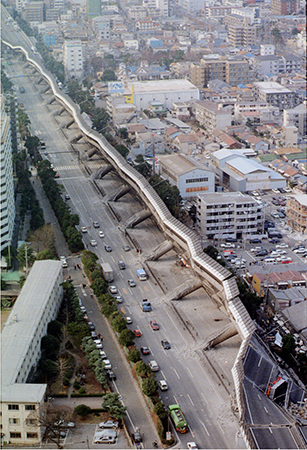
\includegraphics[width=\textwidth]{example1}
		\caption{Plastic hinging at the base of the superstructure associated with collapse - Kobe, Japan 1995 }
		\label{kobe}
	\end{minipage}
	\hfill
	\begin{minipage}[b]{0.4\textwidth}
		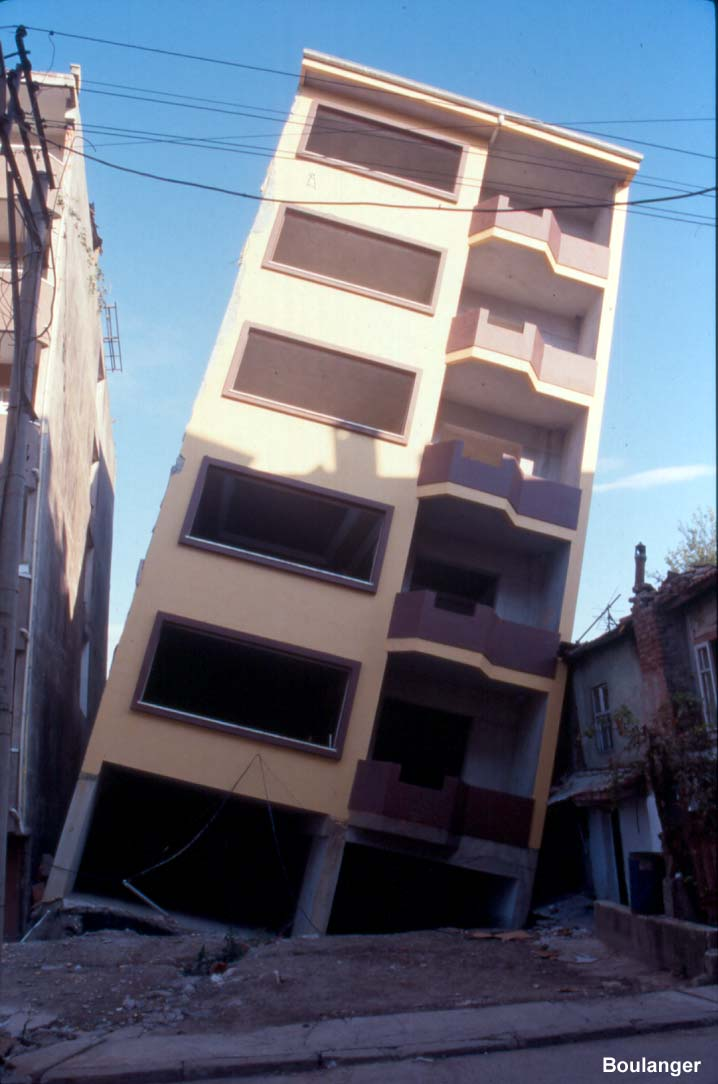
\includegraphics[width=\textwidth]{example3}
		\caption{Unintentional plastic hinging development within the soft soil; large rotations leading eventually to collapse - Adapazari, Turkey 1999}
		\label{turkey}
	\end{minipage}
\end{figure}

The new design philosophy proposes to “contradict” aspects of the conventional design with emphasis on development of plastic articulations within the soil. Strong seismic motion induces large structural inertia forces which, in the case of slender buildings, means larger overturning moments compared to vertical forces. As a result, the footing experiences uplifting at one edge and, possibly, high normal stresses under the opposite edge. If this concentration of stresses is sufficiently large then bearing capacity failure mechanism materializes. In static conditions this phenomena would act detrimental causing failure. However, in dynamic circumstances the cyclic and kinematic effects of the earthquake actually improve the structural performance because:
\begin{enumerate}
	\item The inertial forces change the loading direction rapidly; in the end, it is a cyclic motion so the forces reverse and distress the soil; hence an under-designed foundation ($FS<1$) will experience large displacements during a limited period of time (tenths of a second) but they are reversed before the critical point is reached.
	\item The developing inertial forces should be regarded as an vibratory displacement at the base and not as an external load on the superstructure. Excessive settlements and rotation can be generated as a function of the foundation capacity, however, failure is almost improbable. Thus, the loads transmitted to the superstructure are also restricted to the actual capacity of base or the interface separating the foundation-structure system.
\end{enumerate}

Thus, the main objectives of the new design philosophy focus on foundation response when subjected to seismic motion – a response that opposes the current codes requirements and typically is associated with failure. Thus, the fundamental features of the new method are: 
\begin{enumerate}
	\item Soil uplift and sliding at soil-structure interface is allowed and actually triggered;
	\item Mobilization of bearing capacity failure mechanism due to large over-turning moments;
	\item Plastification of soil near the edges of the footing described by large vertical stresses; 
	\item Combination of any of the above.
\end{enumerate}

The current study works with a collection of peculiar characteristics. First of all, the earthquake is defined as a triggered type, unlike the usual European tectonic one. Moreover, Netherlands national code does not incorporate chapters regarding suitable seismic design simply because it was not the case so far – organizations and companies are currently busy elaborating a proper formulation for this matter. Secondly, the soil is very soft, bedrock lacks at any meaningful depth; the multi-shear waves might amplify the acceleration response at surface, thus the whole assembly describes a unique situation. Thirdly, it would improve the economical aspect, since a reduction in the superstructure ductility demand means a cost reduction regarding the necessary reinforcement required by a conventional capacity design.

Having mentioned all these characteristics, the challenge of this thesis is to apply and examine the new design philosophy effects upon this particular set of aspects. The method proved to be efficient in cases of soft soil responding to the largest earthquake motions of all time; furthermore, it addressed shallow foundations in many tests– which is also the case in this investigation. Instead of taking the standard steps to analyse the dynamic response of the shallow footing, why not adopt this new design philosophy? Why not take advantage of the soft soil prone to accumulate large stresses and use it to limit the ductility demand within the superstructure? 


\section{Research objectives}
Given the complexity of the current application, several limitations are required to be imposed such as:
\begin{itemize}
	\item water is considered at surface level to match the undrained conditions assumption. No pore pressure is accounted for – only total stress analysis conditions are evaluated.
	\item the soil parameters correspond to a homogeneous clay material with linearly increasing properties along the depth which are determined empirically.
	\item no complicated structure is analysed: the foundation-structure system is implemented in Abaqus using a simple geometry: rectangular footing with a lumped mass on top of the slender pier. The emphasis is on the inelastic soil response and not on the superstructure.
	\item only a qualitative comparison with results from scientific literature associated with 2D plane strain conditions is performed, since no real data is available.
\end{itemize}

In order to prepare the final analysis, several previous steps need to be taken:
\begin{enumerate}
	\item Calibration of the material model to match the normalized curves proposed by Darendeli, 2011 \cite{darendeli2001development}.
	\item Examination of one-dimensional site response analysis incorporating the calibrated material model. Validation of results through a comparison between two software: Abaqus and NERA.
	\item Evaluation of inelastic soil responses at surface level when subjected to various values of PGA.
	\item Investigation of the influence of the model boundary conditions on soil response.
\end{enumerate}

Finally, the main scope of the research is to verify whether the new design philosophy is suitable for the ground and seismic conditions specific to Groningen area. This will materialize in an investigation carried out on a soil layer supporting a simple elastic foundation and the main emphasis is on:

\begin{enumerate}
	\item Soil inelastic response: uplift and sliding at soil-structure interface - large settlements and rotation at foundation centre of mass. 
	\item Bearing-capacity failure mechanism: large overturning moments at foundation level.
	\item Soil plastification: large vertical stresses beneath the footing edges.
\end{enumerate}

The effects of such analysis will be compared to the results the researchers group obtained when dealing with similar situations. In case the outcome shows a fair match, it can be speculated that the new design philosophy is successful for this particular set of conditions.

\section{Research outline}
A schematic outline regarding the processes conducted during the thesis project are presented below. 

The study starts with an overview of the new design philosophy to be used in the analyses - a new method that promotes the idea of seismic response going beyond certain thresholds that are commonly associated with system failure. Additionally, it gains knowledge regarding the specific conditions the Northern area of Netherlands reveals, including the particular type of earthquake.

A first step towards the main goal is taken through the calibration of the material model and it is described in Chapter \ref{ch3}. A strain-controlled shear test is simulated through one element mesh;  by applying several strain levels to the shear box it is possible to obtain the non-linear soil response and represent it using normalized stiffness degradation together with material damping curves. The validation consists in comparing the achieved results with the ones existing in the scientific literature.

Chapter 4 extends the previous analysis to a one dimensional soil column subjected to both uniform harmonic as well as real acceleration time history. A site response analysis is performed with emphasis on the inelastic soil outcome in frequency domain together with the site amplification factor. A comparison is performed between Abaqus software ouput and NERA (Non-Linear Earthquake Site Response Analysis) software - in order to validate the model which will assist this investigation further.  In addition, two acceleration time history records  are examined characterised by a higher PGA value and a lower, respectively. Thus, the results can sustain a comparison with the general response assigned for Groningen area expressed in soil amplification hence the validation relates to the context.

In Chapter 5, a finite-element model describes the soil-structure interaction capturing the new design philosophy features (a) soil uplift and (b) mobilization of bearing capacity type of failure. One of the most important aspects of such analysis relates to the boundary conditions associated with wave propagation phenomena. Given the need of reducing the computational expense of the numerical investigation, solutions must offer a good balance between model dimensions and accurate outcome. Various boundary condition options were explored and their effect on the overall inelastic soil outcome. Moreover, the nonlinear ground response is highlighted through interaction curves produced under static conditions and compared to the existing literature. Considering the geometrical nonlinearity associated with the out-rival of the soil-footing interface tensile strength and thus with the uplifting, parametric studies focus on the influence of structural mass dividing the analysis between \textit{(a) lightly-loaded} and \textit{(b) heavily-loaded footings}. In addition, to accentuate the differences between the conventional and the new design philosophy together with the uplifting effect, two other distinctions in terms of soil-footing contact are formulated as (a) Fully Bonded Contact \textit{FBC} and (b) Tensionless Sliding Interface \textit{TSI}.

\begin{figure}[h!]
	\centering
	\includegraphics[width=0.7\linewidth]{"outline"}
	\caption{Overview of thesis outline}
	\label{outline}
\end{figure}

\chapter{Literature survey}
\section{A new design philosophy}

The current chapter presents the particularities of the new approach together with a summary of results and conclusions yielding from numerical models compared to experimental tests (centrifuge tests). The design seems appealing mainly because of current soil conditions Groningen area displays - mostly silty clay layers carrying strip foundations - if the method proves to be successful, it might mark the beginning of a new trend in seismic design research.

It becomes important to understand the effects, benefits and disadvantages of the new method before carrying any analysis. The priority is to examine the inelastic soil response consequences on overall structural assembly, to follow recent research outcome and means of obtaining it. Moreover, a comparison between the two methods help defining advantages, recognize limitations and improvements one method might bring against the other. Let us begin by acknowledging the starting points of the new design philosophy.

\section{Newmark sliding block analogue}
Newmark, 1965 \cite{veletsos1965deformation} proposed a simplified model to examine the dynamic behaviour of earth dams and embankments in terms of permanent deformations, both rotation and settlement. The subject of the study is the analogue of a rigid block positioned on an inclined surface; the focus is on the deformations caused when the inertia forces acting on the sliding mass exceed the frictional resistance of the failure surface. A key parameter is represented by the critical, or yield, acceleration $A_c$ which plays different roles depending on the application. On one example, it depicts the pseudo-static base acceleration $A_c$ generating inertia forces that enhance the \textbf{sliding failure} ($FS=1$) whereas on the other example, it describes the constant base acceleration $A_c$ leading to large over-turning moments, thus to a \textbf{bearing-capacity failure} ($FS=1$). The author showed that when the peak amplitude excitation A exceeds the critical acceleration of the system $A_c$, the underlying medium will only encounter permanent (inelastic) deformations; however, the displacement is not sufficient to provoke failure. A schematization of Newmark model is available in Figures \ref{newmark1} and \ref{newmark2}. Important to mention that these models work in pseudo-static conditions. 

The main lesson learned from Newmark's application is that using an engineering safety factor $F_E$ less than 1 does not necessarily act detrimental on the structure, but it rather leads to a fair performance.
 
 \begin{figure}[!h]
 	\centering
 	\begin{minipage}[b]{0.45\textwidth}
 		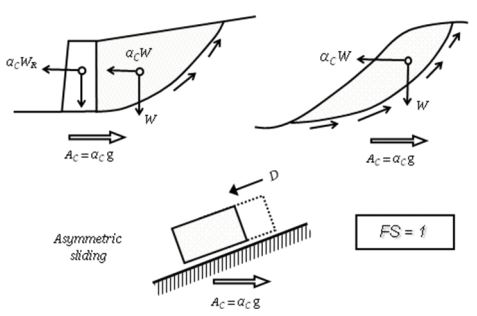
\includegraphics[width=\textwidth]{newmark1}
 		\caption{First example of Newmark model on inclined plane: critical acceleration depicting the sliding failure at the soil-block interface}
 		\label{newmark1}
 	\end{minipage}
 	\hfill
 	\begin{minipage}[b]{0.45\textwidth}
 		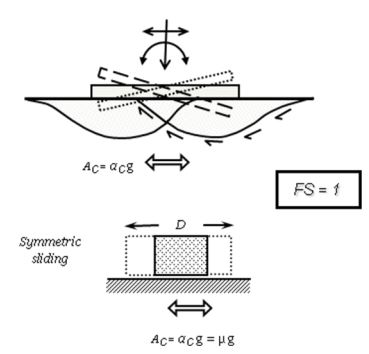
\includegraphics[width=\textwidth]{newmark2}
 		\caption{A second example of Newmark application on horizontal plane: critical acceleration leading to bearing capacity failure}
 		\label{newmark2}
 	\end{minipage}
 \end{figure}
 
 Learning from this concept, Gazetas, 2013 \cite{gazetas2013can} creates two numerical examples that include a safety factor $F_E$ less than unity, focusing on both sliding and bearing-capacity failure.
Firstly, the author investigates the rocking motion of a rigid block highlighting the toppling effect. The object of the study is a rectangular block situated on rigid base with a tensionless interface; details can be seen in Figure \ref{new6}. The excitation comes in the form of Ricker pulse (a representative signal with three main amplitudes) with a peak value exceeding the critical value $A_c$, thus leading to a safety factor:
 \begin{equation}
 F_E= \frac{A_c}{A} \longrightarrow F_E=1/4 \longrightarrow F_E<1
 \end{equation}
 Moreover, the effect of the wavelet frequency gains attention as three various frequencies are introduced ranging from 0.5Hz to 4Hz (representative for the typical ground accelerograms). Results show that the lower frequency produces the maximum angle of rotation $\theta$ with a value close to the "overturning" (or critical) angle $\theta_c$:
 \begin{equation}
 	\theta_c=arctan(b/h)
 \end{equation}
 
 The conclusion states that high frequencies induce less rotation compared to lower frequencies; also, the higher frequency input "barely uplifts the block" hence, assuming an engineering safety factor $F_E$ of less than unity does not imply failure by overturning the slender rigid structures.
  
  \begin{figure}[!h]
  	\centering
  	\begin{minipage}[b]{0.4\textwidth}
  		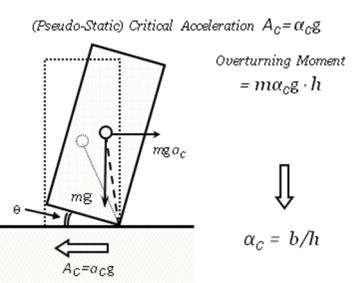
\includegraphics[width=\textwidth]{newmark3}
  		\caption{Representation of rocking rigid block together with a pseudo-static critical acceleration}
  		\label{new6}
  	\end{minipage}
  	\hfill
  	\begin{minipage}[b]{0.55\textwidth}
  		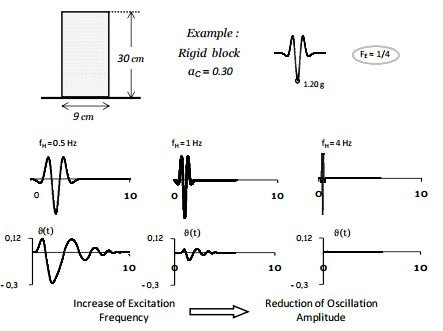
\includegraphics[width=\textwidth]{newmark6}
  		\caption{Representation of Ricker pulse. Input frequencies (0.5Hz - 4Hz) and the outcome in terms of angle of rotation $\theta$}
  		\label{newmark6}
  	\end{minipage}
  \end{figure} 
 
 \newpage
  Furthermore, Gazetas analysed a simple one-bay building frame subjected to low frequency acceleration record corresponding to Kocaeli earthquake (Turkey, 1999) - the choice of a low frequency motion corresponds to a large angle of rotation as it was discussed in the previous example. The aim of the study is to highlight the mobilisation of soil failure. The author incorporated the pseudo-static critical acceleration $A_c$ that Newmark proposed and calculated the safety factor in terms of accelerations:
 \begin{equation}
 F_E= \frac{A_c}{A} \longrightarrow F_E=1/3 \longrightarrow F_E<1
 \end{equation}
 where $A_c$ is the critical acceleration leading to large overturning moments $M$ and shear forces $Q$ on the foundation which, in combination with the vertical force $N$, lead to the bearing capacity failure. And $A$ is the peak ground acceleration of the input record, here $A=0.36g$. Figure \ref{new5} shows the configuration of the model.
 
   \begin{figure}[!h]
   	\centering
   	\begin{minipage}[b]{0.45\textwidth}
   		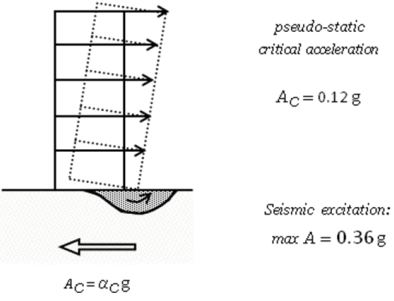
\includegraphics[width=9cm, height=12cm, keepaspectratio]{newmark5}
   		\caption{Representation of bearing-capacity failure of a one-bay building frame associated with a $F_E<1$}
   		\label{new5}
   	\end{minipage}
   	\hfill
   	\begin{minipage}[b]{0.45\textwidth}
   		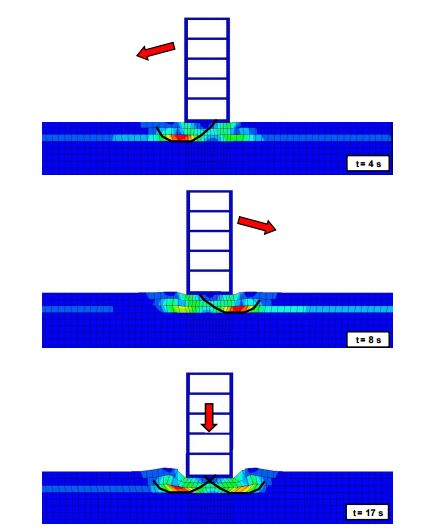
\includegraphics[width=\textwidth]{newmark4}
   		\caption{Soil response of a building frame subjected to acceleration record with A=0.36g. The shear stress contours indicate the failure zones at different times}
   		\label{new4}
   	\end{minipage}
   \end{figure} 
  
 The results of the analysis can be seen in Figure \ref{new4}. It can be concluded that, indeed, failure mechanisms develop within the underlying soil; however, due to the cyclic nature of the seismic motion, the "failure" does not take long and is cancelled by the trend in opposite direction. The third snapshot (at t=17s) represents the end of the earthquake and it shows that the final outcome is a combination of settlements and permanent rotation. This might be acceptable in many cases; still, it is the responsibility of the structural engineer to decide the critical deformations.
 
 
 Nevertheless, the entire phenomenon requires more attention to the details - the chapter continues with a description of non-linear aspects emerging from such dynamic application.
  
  \newpage
\section{Non-linear soil response - Effects}
During seismic loading, the soil responds in a non-linear fashion; studies (Gazetas, 2004 \cite{gazetas2004nonlinear}, Apostolou, 2012\cite{apostolou2011soil}) highlight three mechanisms that might occur in case of ground shaking as the figure below shows. Moreover, one can recognize two types of nonlinearities that govern the response - \textbf{geometrical} and \textbf{material}.

Geometrical nonlinearity can be described as the separation at supporting soil-strip footing interface that it usually addressed as \textit{uplifting}. The material nonlinearity refers to the type of failure mechanisms governed by the bearing capacity mobilization induced by large cyclic overturning moments - also known as \textit{soil failure}. 

\begin{figure}[h!]
	\centering
	\includegraphics[width=0.7\linewidth]{"nonlin"}
	\caption{Types of nonlinearity}
	\label{types}
\end{figure}

Scientific literature (Chopra, 1985 \cite{chopra1985simplified}, Pecker, 2001 \cite{cremer2001cyclic}, Gazetas, 2013 \cite{gazetas2013can}) describes several types of possibilities of nonlinear soil-foundation response in terms of both geometric nonlinearity (uplifting and sliding) and material inelasticity (soil yielding) and it can be studied using the following methods:
\begin{itemize}
	\item 	Winkler method - comprises the settlement-rotation at the base of the foundation which is described as a series of dashpots and springs. The structure was described by a beam on an elastic medium;
	\item 	advanced macro-element modelling - the whole soil-structure system is described by an unique element which simulates the generalized force-displacement behaviour of the foundation. It is worth noting that in the elastic range, and without uplifting, the macroelement reduces to the familiar dynamic spring and dashpot(impedance) matrix;
	\item direct methods (finite element or finite difference methods) that successfully simulate both the soil and the foundation and the contact surface between them. This method is currently used as it proves itself efficient and accurate.
\end{itemize}

\section{Geometrical non-linearity: Uplifting}
New philosophy not only allows one of the nonlinearity behaviour to develop within the soil but also encourages that design should apply a safety factor against uplifting and soil \mbox{failure} lower than unity. This way, the structure ductility demand will decrease \mbox{considerably}, optimizing the energy dissipation path throughout the building. Various studies focused on the rocking response simulating the soil in different manners; for example, the first models described the rigid soil via tensionless spring-dashpot elements (Chopra \& Yim 1985 \cite{chopra1985simplified}, Koh et al, 1986 \cite{koh1986harmonic}) followed by a single macro-element which includes a constitutive law that accounts for the uplift mechanism in a soil-foundation system. Ultimately, the dynamic analysis is performed in finite-element based software ( Hibbit et al, 2001 \cite{hibbett1998abaqus}, Gazetas et al, 2010 \cite{anastasopoulos2010soil}) - the model combines a rigid foundation footing, elasto-plastic soil and an advanced contact algorithm that inserts the potential sliding and uplifting.

The geometrical non-linearity is generated when large overturning moments (associated with uplift) or lateral forces (inducing sliding) act on the footing. Uplifting occurs due to the incapability of the soil to withstand tensile stresses and it materializes through loss of contact at soil-foundation interface. Additionally, it dictates the moment-rotation relationship towards a softening behaviour even under elastic conditions.

Early studies (Meek, 1975 \cite{meek1975effects}, Chopra \& Yim,1985,  \cite{chopra1985simplified}) considered a simplified rigid soil model and highlighted two states of response: (1) full-contact stage and (2) uplifting stage. A transition between the two phases relates to the bending capacity the structure displays. For a rectangular shallow foundation under static conditions, the moment capacity of the structure right before the initialization of the uplift is:
\begin{equation}
	M_{ult}= \frac{N B}{2}
\end{equation}
 where $N$ is the permanent axial force on the footing, $B$ is the width of the foundation. The load is assumed to be applied with an eccentricity equal to the half-span of the footing (B/2). 
 
 Further, the maximum overturning moment induced by inertial forces is:
 \begin{equation}
 	M_{max}= N \frac{a}{g}\frac{H}{2}
 \end{equation}
where $a$ is the PGA value, $g$ is the gravitational acceleration ($g=9.81m/s^2$), $H$ is the height of the superstructure.

Now, the criterion for uplifting is expressed as a function of these two moments; particularly, if the maximum overturning moment goes beyond the capacity ($M_{max}>M_{ult}$), then toppling of the structure occurs. This statement is true for static conditions while in dynamic conditions the uplifting acts beneficial. This is because the foundation can withstand higher values of bending moments compared to the ultimate capacity, $M_{ult}$. The key in this rocking behaviour is the relatively short time period in which the stresses surpass the limiting values. The ground acceleration displays a rapid change in trend which makes the foundation block to decelerate, stop and rock in the opposite direction. Researchers (Gazetas, 2013 \cite{gazetas2013can}) showed the correlation between the natural period of the foundation footing and rocking potential: high frequency seismic motion leads to a somehow "safer" rocking response preventing collapse or toppling of the superstructure as section 2.2 also justifies.

Scientific literature (Gazetas et al, 2013 \cite{gazetas2013nonlinear}, Apostolou, 2011 \cite{apostolou2011soil}, Faccioli et al, 2001 \cite{faccioli2001investigation}, Anastasopoulos et al \cite{anastasopoulos2010soil} etc.) confirms that the nature of the seismic excitations along with the fundamental period of the structure dictate the response of the soil-foundation system via a more complicated material model that allows for soil yielding. 

One important aspect to keep in mind is that uplifting systems experience larger rotations and occasional overturning whilst the sliding system resists the strong seismic motions with large permanent displacements.

\begin{figure}[h!]
	\centering
	\includegraphics[width=0.7\linewidth]{"rocking"}
	\caption{The geometrically non-linear nature of the problem is evident even under the assumption of an elastic soil. The image confirms the conclusions from both earlier and more recent models }
	\label{rocking}
\end{figure}

\section{Material non-linearity: Soil yielding}
In dynamic conditions, the soil response is generally inelastic, hysteretic and irreversible. Pecker and Pender, 2000 \cite{pecker2000earthquake} proposed a model in which the underlying medium was divided into two main areas: \textit{near field} and \textit{far field} - Figure \ref{near} shows a configuration of their model. The authors described how the sub-domains display slightly different soil non-linear response:

\begin{itemize}
	\item \textit{near field} - represents the soil in the proximity of the foundation where it encounters both the seismic signal and the stress concentrations caused by the vibrations of the structure. 
	\item \textit{far field} - represents the soil located far enough from the structural system such that it experiences only seismic waves propagation.
\end{itemize}
 
\begin{figure}[h!]
	\centering
	\includegraphics[width=0.7\linewidth]{"nearfar"}
	\caption{Schematization of Pecker\&Pender model, 2000}
	\label{near}
\end{figure}

The near-field domain is governed by the material non-linearities. Seed and Idriss,1986	\cite{seed1986use} first introduced the concept of equivalent linear analysis focusing on the non-linear soil response. Using a linear, wave propagation analysis, it updates the visco-elastic soil properties (shear stiffness and damping ratio)in an iterative fashion. The method is valuable for determining the stress state in far-field domain; however, it is not suitable for the near-field as it fails to estimate the plastic strains caused by the footing oscillations. The level of these strains can reach a considerable amount if the foundation experiences large overturning moments.

Thus, the need of a more advanced material model able to incorporate such effects. Starting from late '60s, numerous constitutive models have been proposed describing the non-linear characteristics. First models focused on a elasto-(visco)-plastic material model which further included features such as isotropic plastic hardening rules; these models are adequate if only loading occurs with moderately unloading - which is not necessarily the case. Hence, the situation calls for an constitutive model upgrade integrating hysteresis effects while combining the isotropic and kinematic plastic hardening rules. One of the remarkable material models was proposed by Mroz and Iwan,1967 \cite{mroz1967description} - it represents the continuous yielding via multiple yield surfaces in stress space. The constitutive model offers a powerful and flexible calculation tool when combined with kinematic and isotropic hardening/softening plastic rules.

Lemaitre and Chaboche, 1994 \cite{lemaitre1994mechanics} gather the conceptual work of the last decades, providing an inventory of constitutive models for continuum mechanics and thermodynamics. Among many others, the book investigates aspects of plasticity, out of which a \textit{non-linear kinematic hardening rule} drew the attention of the current thesis.

\begin{figure}[h!]
	\centering
	\includegraphics[width=0.8\linewidth]{"uplift"}
	\caption{Mobilization of ultimate bearing capacity; uplifting(a) and soil yielding (b)}
	\label{uplift}
\end{figure}

The following section will present in more detail the adopted constitutive model which successfully integrates hysteretic features as well as kinematic hardening rules.

\newpage
\section{Soil condition}
\subsection{Problem statement}
The current situation deals with a relatively weak clay layer, typical to northern area of Netherlands - the rock layer lacks in most of the cases, being replaced by dense sand deposits. The clay is characterised by little friction angle, cohesive properties as well as low Young's modulus values and, implicitly, low shear wave velocity - amplification of the seismic motion can be expected when dealing with such soil properties.

Appendix \ref{App:AppendixA} shows a sample of CPT taken in the area of interest - which confirms the assumption of predominantly clayey soil with pockets of silty sand of medium strength. Such soil conditions associated with this type of induced earthquake define a new unique situation that requires its own seismic design approach.

\subsection{Constitutive model}
\paragraph{General} A first step in deciding the implementation of the material model is understanding the application to be investigated - what phenomena happens, what are the effects, what mitigations does it require. Having in mind the dynamic nature of the problem, the material model should enclose features that are able to describe mechanically the non-linear phenomena. 

As the former section explained, the near-field sub-domain is governed by both the inelastic soil response caused by seismic waves propagation and stress concentrations developed underneath the footing. The situation calls for an advanced constitutive model able to accurately integrate the hysteretic effects, the isotropic and kinematic hardening rules.

Lemaitre and Chaboche, 1994 \cite{lemaitre1994mechanics} developed such material model discussing the behaviour of both sand and undrained clay soils. Nowadays, research trend (Gazetas et al. \cite{gazetas2004nonlinear}, \cite{gazetas2013nonlinear}, \cite{anastasopoulos2010soil}) comprises the nonlinear kinematic hardening model characterized by a von Mises failure criterion along with an associated flow rule. The description of the model is rather accessible as it requires only Young's modulus $E$, soil yield stress $\sigma_y$ and strength $\sigma$. The research group performs multiple analyses using the software ABAQUS; the FEM program incorporates the non-linear kinematic hardening rule in the material section and it yields satisfying results. Moreover, they suggest a simplified constitutive model designated for studying the cyclic response of shallow foundation (Anastasopolous, 2011 \cite{anastasopoulos2011simplified}); the validation includes experimental work such as large-scale tests on a square footing resting on a loose sand and centrifuge tests of shallow footings on clay and sand. Results highlight that von Mises failure criterion is a trustworthy material model for clay in undrained conditions; also, the numerical and experimental models are were capable of accurately process the lateral cyclic performance and the lateral capacity of the footing. The vertical loading led to similar effects on the footing, thus it can be concluded that the current constitutive model represents a fair choice for this particular problem. One of the material model limitations stand in its incapacity of acquiring pore pressure build-up nor dissipation effects. Yet, it proves safe to assume an undrained behaviour given the short duration of seismic loading applied on the system. Figure shows a sample of results obtained by Anastasopoulos (\cite{anastasopoulos2011simplified}).

\begin{figure}[!h]
\centering
	\includegraphics[width=0.5 \linewidth]{"exper"}
	\caption{Validation of the numerical model against the centrifuge test of a square footing resting on clay. Large vertical loading on the foundation to generate bearing capacity type of failure. The inelastic soil response is expressed in terms of moment-rotation relationship and uplifting potential}
	\label{experimental}
\end{figure}

\paragraph{Plastic models} Generally, materials experience irreversible deformations when elastic limit is reached but loading persists. Theory of the elasticity explains the occurrence of slip surfaces caused by instabilities via the time-independent irreversible deformations. Moreover, it determines the permanent deformations that lead to collapse preventing them while investigating the stability of the system. 
In order to create a plasticity model, there is the need of few features such as:
\begin{itemize}
	\item a yield criterion\
	\item a strain hardening rule\
	\item a plastic flow rule\
\end{itemize}

Simplifications of this constitutive models tend to responsibly neglect anisotropy and \mbox{temperature} independence aspects. Important to mention that the term \textit{kinematic} refers to criteria evolution while textit{isotropic} relates to flow and hardening criteria. Linear kinematic hardening rules provide the translation of the loading surface making use of the hardening variable which indicates the position of the loading surface. However, its limitations call for a more advanced model able to capture the nonlinearity caused by the kinematic hardening. For instance, the linear hardening rule fails to assess the relaxation effects induced by average stresses or the ratcheting effect. In addition, stabilization occurs accordingly to a perfectly plastic cycle when subjected to prescribed strains which does not happen in reality.

Henceforth, the evolution of stress in nonlinear conditions includes two components:

\begin{itemize}
	\item 	isotropic hardening component which based on the plastic deformation defines the size of the yield surface giving information related to the change in the equivalent stress;
	\item 	nonlinear kinematic hardening component which contains a purely kinematic term and a relaxation one describing the translation of the yield surface.
	\end{itemize}
	
	
Considering all above, von Mises failure criterion can be briefly described using three main equations:
\begin{equation}
\sigma_y = \sqrt{3}S_u
\end{equation}
\begin{equation}
\sigma_y = \frac{C}{K}+\sigma_0
\end{equation}
\begin{equation}
K=\frac{C}{\sqrt{3}S_u-\sigma_0}
\end{equation}

where C is the initial kinematic hardening parameter, K is the parameter characterizing the rate of reduction of the kinematic hardening with increasing plastic deformation, $\sigma_y$ is the maximum yield stress, $\sigma_0$ represents the yield stress at zero plastic strain and $S_u$ is the undrained shear strength. 

A more detailed description of the constitutive model can be found in Appendix \ref{App:AppendixB} in terms of stress state, failure criterion development and mathematical formulas.

\section{Numerical analyses}
\subsection{General features}
Researchers (Anastasopoulos, \cite{anastasopoulos2014simplified}, Ntritsos et al, 2015 \cite{ntritsos2015static}, Panagiotidou, 2012 \cite{panagiotidou2012pushover}) \mbox{developed} various models that highlight the new design particularities - both two-dimensional and three-dimensional elements were used in order to elaborate the soil-foundation system behaviour in static, cyclic and dynamic load combinations. 

All the FE analyses performed to research this approach were formulated using the software \textit{Abaqus} \cite{manualversion}. Both the soil and the foundation are modelled as eight-noded hexahedral brick-type element, the soil being considered a non-linear element while the latter elastic. Additionally, centrifuge tests and experiments are compared with the numerical outcome for validation purposes.

Numerous simulations included a saturated clay type of material characterised by an undrained shear strength $S_u$ and a maximum shear modulus $G_{max}$. It proves appropriate to consider undrained soil behaviour due to the rapid loading that corresponds to the seismic excitation - in addition, it allows a total stress analysis which can be described using a von Mises failure criterion along with an associative flow rule. The inelastic soil response was described through an evolution law based on both nonlinear kinematic hardening and isotropic hardening components that account for the changes the yield surface experiences within the stress state.

The two main components of the structural system were separated through an interface that permits sliding and uplifting - a special contact algorithm dictates the detachment in the specific areas where the angle of rotation exceeds the foundation characteristic critical rotation $\theta_c$. The boundaries, both lateral and vertical, depend on the loading type the structure experiences - static conditions do not impose special requirements regarding the position of the boundaries. However, dynamic conditions introduce the wave propagation effect that might distort the final results due to reflections. Two boundary options are proposed - the first one assumes the bounds at a considerable distance from the foundation such that the reflected waves do not influence the results. The second one places the bounds in a position consistent with the static conditions - the trick is to add "lateral infinite elements" that absorb the propagated waves and have similar effect with the first option. The location of the later borders accounts for the pressure-bulbs generated by the dissipation of vertical stresses induced by the moment loading on the foundation strips. Figures \ref{2d} and \ref{3d} show examples of FEM models incorporating all the features formerly described.


\begin{figure}[!h]
	\centering
	\begin{minipage}[b]{0.45\textwidth}
		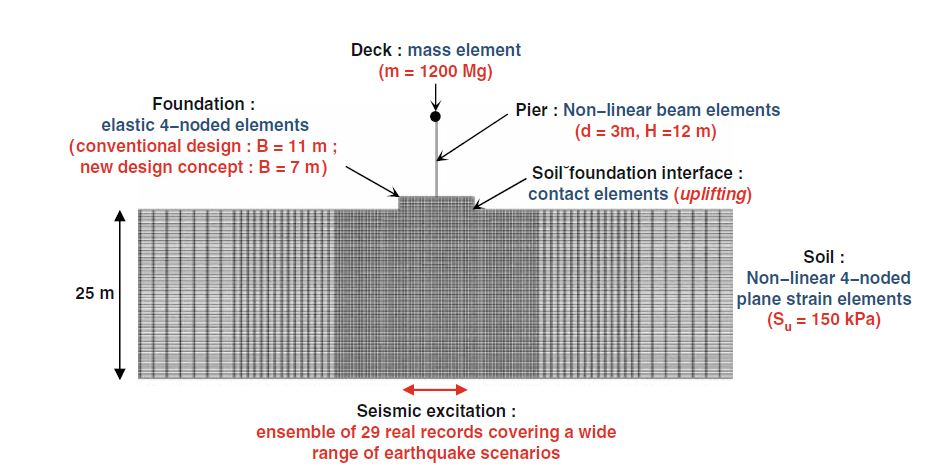
\includegraphics[width=\textwidth]{scheme2D}
		\caption{Overview of the finite element modeling: plane-strain conditions are assumed, taking account of material (soil and superstructure) and geometric nonlinearities}
		\label{2d}
	\end{minipage}
	\hfill
	\begin{minipage}[b]{0.45\textwidth}
		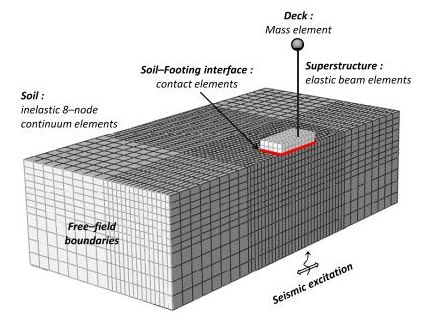
\includegraphics[width=\textwidth]{3d_model}
		\caption{Rigorous 3D FEM model comprising the soil-footing-structure system accounting for material and geometric nonlinearities}
		\label{3d}
	\end{minipage}
\end{figure} 

\newpage
\subsection{Conventional versus new design philosophy}
The whole design research started with a comparison between the conventional and new design philosophy when subjected to various acceleration time histories. Figure \ref{conventional2} shows the results for a situation with moderate seismic input corresponding to Kalamata earthquake, 1986 whereas Figure \ref{conventional} shows the distinction between the two alternatives when considering a stronger earthquake (Kobe, 1995). All the assumptions aforementioned are valid for these analyses. The conventional design premises correspond to the ones described in section 1.2.1 whilst the later method characteristics are depicted in section 1.2.2. Moreover, the capacity design includes an overstrength factor of safety for seismic loading $\gamma_{Rd}=1.4$ dictating the position of the plastic hinge at the pier base. On the other hand, the under-designed foundation, corresponding to the new design, is assigned with an understrength factor of safety $1/\gamma_{Rd}=0.7 <1$. 


\paragraph{Medium earthquake motion}
Few remarks can be formulated based on the observed results. The first set of plots highlight the elastic response of the footing when conventional design is considered whereas the new design shows highly inelastic response. The non-linear response comes at the cost of large settlements under the foundation as the second plot shows; on the contrary, the elastic foundation and pier yielding prevent such consequences. Furthermore, the conventionally designed pier experiences \mbox{inelasticity}, however in tolerable limits while in the new design scheme, the pier remains mainly elastic thanks to soil yielding. Finally, the deck drift, or horizontal displacement at mass, is on one hand caused by the flexural pier distortion (here, $\Delta c$) while on the other hand is due to foundation rotation ($\Delta r$). 

\paragraph{Strong earthquake motion}
The investigation is further extended to include a stronger earthquake motion which is exceeding the design limits (the Takatori accelerogram recorded at Kobe, 1995). This acceleration time history is relevant as it represents one of the most disastrous earthquakes of the recent times (PGA=0.7g, PGV=169cm/s); the simplified structural system corresponds to a section of Hanshin Expressway which partly collapsed during the earthquake. The results of the two alternatives can be visualized in Figure \ref{conventional}.

Similar conclusions can be drawn from this comparison; the deformed mesh plots make the position of the "plastic hinging" quite evident: the capacity designed system experiences large curvature at the base of the pier and little inelastic deformation at the soil level whereas the other alternative shows opposite effects. The accumulation of stresses beneath the foundation (the extended red areas) hints the bearing capacity type of failure expected from the under-designed footing. The curvature recorded at pier level clearly indicates collapse for the conventional case and elastic response for the other. These effects are linked with the deck drift $\Delta$: large horizontal displacement at the top of the pier is observed in contrast with limited deck drift for the second alternative. Additionally, the moment-rotation at foundation level corresponds to the soil response: on one hand, elastic foundation response as the pier failure limits the transmitted stresses towards the soil and, on the other hand, inelastic response associated with bearing capacity failure mechanism. As consequences, the conventional designed foundation experiences small settlements at soil level (approx. 7cm) when the other method reveals increased foundation settlements (24cm). As Anastasopoulos, 2010 \cite{anastasopoulos2010soil} acknowledged "\textit{...although such settlement is certainly not negligible, it can be considered as a small price to pay to avoid collapse under such a tremendous ground shaking}".

\begin{figure}[!h]
	\centering
	\includegraphics[width=0.9\linewidth]{"conven2"}
	\caption{Distinction between capacity design and new design philosophy when subjected to a medium earthquake signal (Kalamata, 1985); (a) moment-rotation relationship at foundation level; (b) settlement-rotation response of the footings; (c) bending-moment curvature response at the pier base; (d) time history of deck drift $\Delta$}
	\label{conventional2}
\end{figure}

\begin{figure}[h!]
	\centering
	\includegraphics[width=0.8\linewidth]{"conventional"}
	\caption{Comparison between the two design alternatives for strong seismic signal; (a) deformed mesh indicating the location of plastic hinging zones; (b) bending moment-curvature response at pier base level; (c) time history of deck drift}; (d) overturning moment-rotation relationship at foundation level; (e) foundation settlement-rotation response.
	\label{conventional}
\end{figure}



\newpage
\subsection{Relevant studies}
Now, that the main differences in response were evaluated, it is important to select \mbox{relevant} cases from the vast collection of studies performed to support the new design philosophy. Various methods of simulating dynamic response were examined for systems considering slender structures simplified as rigid oscillators standing on inelastic soil. The system response was further processed in order to obtain an approximation of the rocking \mbox{behaviour}: moment-rotation response together with settlement-rotation are of main \mbox{interest}. In addition, emphasis on the nonlinearities effects were made with respect to the fundamental period of the oscillator.

\paragraph{Monotonic response}
The monotonic test represents a simplified technique to estimate the dynamic response; it comes in the form of a "push-over analysis" and it gained popularity for being able to accurately estimate the seismic deformation demands and ultimate capacity. The concept consists in applying a monotonically increasing lateral displacement loading at superstructure level until failure by overturning is reached. 

\paragraph{Cyclic response}
The cyclic tests act in accordance with the previous concept; in fact, it is known as "cyclic push-over test". A rather rotation-controlled loading is applied on the same location in superstructure to simulate the cyclic effects: the rotation is applied through a lateral displacement associated with a constant cyclic amplitude.

\paragraph{Dynamic response}
Finally, the seismic response is generated via a series of ground-shaking accelerograms - both medium and strong earthquakes recorded all around the world (Kalamata, 1986; Kobe, 1995; Lefkada, 2003, etc). The dynamic input was introduced at bedrock level whilst the response was extracted at the base of the structure.

Furthermore, all simulations examined the difference in response between lightly and heavily loaded foundation expressed in terms of safety factors. The former situation translates into a high vertical safety factor $FS_v=5$ whereas the later assumes a low value $FS_v=2$. *The vertical safety factor $FS_v$ is defined as the ratio between the ultimate bearing capacity under pure vertical static load $N_u$ and the currently applied axial force $N$ - $FS_v = \frac{N_u}{N}$. 

\begin{figure}[!h]
	\centering
	\includegraphics[width=0.8\linewidth]{"largeFS"}
	\caption{Distinction between lightly and heavily loaded foundation highlighting the effects on the soil response}
	\label{largeFS}
\end{figure}

\begin{figure}[!h]
	\centering
	\includegraphics[width=0.9\linewidth]{"staticpush"}
	\caption{Comparison between the soil response when subjected to monotonic/cyclic/ seismic loading; moment-rotation response for (a)FSv=5 and (b) FSv=2}
	\label{pushover}
\end{figure}

\begin{figure}[!h]
	\centering
	\begin{minipage}[b]{0.4\textwidth}
		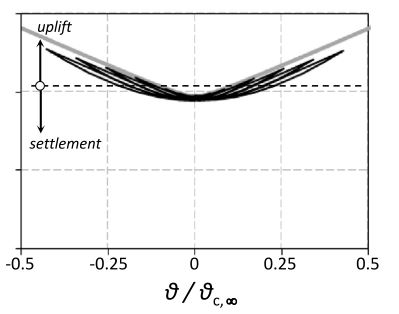
\includegraphics[width=\textwidth]{settle}
		\caption{Settlement-rotation relationship for FSv=5 (lightly loaded foundation) (gray line corresponds to monotonic backbone curve)}
		\label{set}
	\end{minipage}
	\hfill
	\begin{minipage}[b]{0.45\textwidth}
		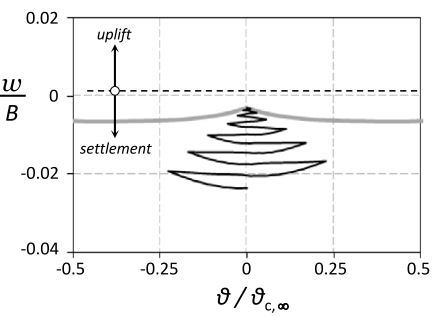
\includegraphics[width=\textwidth]{settle2}
		\caption{Settlement-rotation relationship for FSv=2 (heavily loaded foundation (gray line corresponds to monotonic backbone curve)}
		\label{set2}
	\end{minipage}
\end{figure} 

\newpage
Figures \ref{largeFS}, \ref{pushover}, \ref{set} and \ref{set2} show a collection of responses with emphasis on the inelastic response; several remarks can be made regarding the differences in outcome and the correlation with the vertical safety factor, as it follows:

\begin{itemize}
	\item the lightly loaded foundation displays an uplifting-dominated response compared to the sinking-dominated response associated with the heavily loaded foundation (see fig \ref{largeFS});
	\item for the former situation, the cyclic moment-rotation envelope is well comprised within the static push-over one (see fig \ref{pushover} (a1)) - it relates to the low dissipated energy. The cyclic loading causes small deformations - as a consequence, the area underneath the footing edges shows progressive recession (small downward settlements and considerable degradation of rotational stiffness) - see fig \ref{set}. 
	\item in contrast, the highly loaded foundations experience a different trend: the moment-rotation envelope does not follow the static conditions anymore. As the safety factor increases, the soil encounters an accumulation of downward settlements; furthermore, bearing capacity failure mechanism is evident since excessive shear deformation occur;
	\item the deformation of the lighly loaded footings is roughly elastic whereas the heavily loaded exhibit a strongly inelastic response - this means gradual accumulation of plastic deformation leading to higher residual rotations.
	\item the results of the cyclic push-over analysis match the seismic analysis outcome. The soil high compliance leads to large deformations and, thus, the bearing capacity failure mechanism becomes apparent.
\end{itemize}

In the same train of ideas, the rotational capacity expressed in terms of ultimate moment resistance of the footing $M_{ult}$ relates to both the axial force $N$, and the shear force $Q$ acting on the foundation. Recent research emphasize on elaborating ultimate limit states defined by combinations of $N, Q$ and $M$ loads - the \mbox{graphical} representation is known as \textit{failure envelope}.
	 
Another of the new concept goals stands in defining this failure locus - based on load combinations and their position regarding this envelope, one can state whether the foundation acts stable or not. Many experiments based on model-scale shallow footing support this theory along with theoretical and numerical failure equations (Murff, 1994, Bransby and Randolf, 1998 \cite{bransby1998combined}, Butterfield and Gottardi, 1994 \cite{gottardi1999plastic}). Experiments (Gajan et al, 2005 \cite{gajan2005centrifuge}) highlight the influence of two \mbox{parameters} governing the load displacement and energy dissipation aspects of the soil-foundation interface during cyclic loading: static factor of safety regarding vertical force exclusively (FSv) and moment-to-shear ratio - together describing the load path. Henceforth, a challenge in assessing seismic loading impact represents the correct evaluation of loading combination (shear force $Q$ and overturning moment $M$) that will lead to failure for a given vertical force, $N$, acting on the superstructure.

 Among many others, Nitros et al, 2015 \cite{ntritsos2015static} describe such failure envelopes highlighting the importance of the foundation aspect ratio and vertical safety factor. One feature relates to the types of interface available for the analysis and two conditions are taken into consideration as it follows:
\begin{enumerate}
	\item Fully bonded contact [FBC] - the foundation remains in perfect contact throughout the entire analysis; this condition prevents sliding and separation of the foundation from the surrounding soil because of the infinite tensional and shear capacities of the interface.
	\item Tensionless sliding interface [TSI] - allows sliding at the contact surface as well as separation of the foundation; the interface follows Coulomb's friction law in total stress depending on the adhesion coefficient $\alpha$.
\end{enumerate}

Many studies focused on the importance of the combined $NQM$ loading and individual effects of the forces susceptible to act on the foundation at certain points. Yun \& Brandy, 2007 and Gouvernec (2008) \cite{randolph2011offshore} formerly examined the undrained bearing capacity of rigid embedded strip foundations under combined $NQM$ loading using a fully bonded contact, followed by Ntritsos et al (2015) who extended the studies to three-dimensional problem of squared foundations adding the option of a tensionless sliding interface.

\begin{figure}[h!]
	\centering
	\includegraphics[width=0.8\linewidth]{"failure"}
	\caption{Combination of loads applied at the reference point of on shallow foundation; schematisation of the failure envelope in 2D and 3D space according to Randolph\& Gouvernec, 2007 \cite{randolph2011offshore}} 
	\label{fail_contour}
\end{figure}

Nevertheless, the two maximum values - horizontal load $Q_{max}$ and overturning moment $M_{max}$ do not solely represent the failure mechanism; infinite combinations of $Q$ and $M$ are comprised within a failure envelope plotted against normalized values. Additionally, the effect of the vertical load which influences the $QM$ interaction was set to $N=0$. The figure beneath displays the four main points on the envelope that represent different loading conditions together with significant output at carefully selected points. Both the fully bonded contact (FBC) and tensionless sliding interface (TSI) conditions were investigated and presented for comparison. Important to mention is that the authors preferred to normalize the $Q$ and $M$ values in accordance to the foundation width $B$, area $A$ and undrained shear strength $S_u$ - the plot contains on the x direction $Q/AS_u$ whilst for the y direction it has $M/BAS_u$. 
The main points have specific characteristics as it follows:
\begin{itemize}
	\item \textbf{Point A} \textit{pure moment loading $M_{ult}$;} in this point, shear force $Q=0$. A scoop-type of mechanism is noticeable along with the plastic shear strains shadow contours. Negative rotation can be observed from both the embedded plot as well from the graph.
	\item\textbf{Point B} \textit{pure rotation $M_{max}$;} the tangent line to this point is parallel to the horizontal axis which acts accordingly to the associated flow rule which dictates preservation of normality. Given the dependence of moment loading, the mechanism is characterized by the scoop shape as well. The foundation response is mainly rotational with negative horizontal translation.  
	\item\textbf{Point C} \textit{pure horizontal translation $Q_{max}$;} also, the preservation of normality can be noticed in the form of the tangent line which is parallel to the vertical axis. The failure mechanism is characterized by the sliding of the whole system; both active and passive sides exhibit failure as presented above - including the side walls effects.
	\item\textbf{Point D} \textit{pure horizontal load $Q_ult$;} reversed scoop mechanism is observed with the centre of rotation close to the soil surface - the failure mechanism equally depends on both the horizontal translation and counter-clockwise rotation.
\end{itemize}

The herewith figures correspond to the two types of interface - FBC and TSI. There are certain dissimilarities between the two contact surfaces effects - few are exposed as it follows:
\begin{itemize}
	\item First, the failure mechanisms partly coincide with the ones earlier described in terms of the four limit points (A-D). The sliding faces only constrain the extent of the failure surface leading to no foundation-soil contact which lead to a prevention of wedge development.
	\item Moreover, the response associated with point B - pure rotation - is different compared to FBC which displays a scoop mechanism; a rather wedge type of failure is evident. Besides, the mechanism at lateral sides, corresponding to the sidewalls, and below the foundation strip seem half of the previous contact situation (FBC).
	\item Consequently, the sliding and separation of the foundation from the soil is permitted. This leads to a reduction in displacement - just about 1/2 compared to fully bonded contact. Additionally, the ratio D/B which describes the footing geometry and depth (D - height, B - width), varied within the analyses allowing the researchers to observe the influence of embedment on the Q-M failure envelopes. 
\end{itemize}

\begin{figure}[h!]
	\centering
	\includegraphics[width=0.8\linewidth]{"fbc_contour"}
	\caption{Failure envelope for a fully bonded contact problem together with the deformation contours; the solid dot represents the rotation pole}
	\label{contour}
\end{figure}

\begin{figure}[h!]
	\centering
	\includegraphics[width=0.9\linewidth]{"MQN"}
	\caption{Failure envelope for a tensionless sliding interface problem highlighting the main failure mechanism points; the deformation contours for each position on the failure envelope; the solid dot represents the rotation pole}
	\label{MQN}
\end{figure}

\newpage
\section{Numerical tools - ABAQUS}
Abaqus \cite{hibbett1998abaqus} offers a wide range of elements and features that help achieving a nonlinear analysis regardless the domain or simulation expertise - it's attractiveness stands in the possibility of customization, making the software extremely flexible, yet meticulous. 

Abaqus has been chosen as the finite element analysis software in this study for the following
reasons: First, it serves well the geotechnical engineering goals as it provides soil and structural elements, total and effective stress analysis, consolidation, static and dynamic analysis and many more. Second, a Von-Mises yield criterion is readily available. Moreover, it has capability to conduct two dimensional plane strain analyses. Finally, literature studies on this particular geotechnical problem using this software are available as well (see Gazetas et al \cite{gazetas2013can}, \cite{anastasopoulos2010soil}, \cite{anastasopoulos2014simplified}, etc)- thus, a relevant comparison can be made without additional effort. 

It offers several packs of database, out of which Abaqus/Standard seems the most suitable. It represents a model database appropriate for both linear and nonlinear static, linear and/or low-speed nonlinear dynamic situations in which stress solutions have a great significance. Through iterative procedures and convergence algorithms, the unknown variables are determined based on the current available information - thus, it becomes computationally expensive when it does not reach the equilibrium. Two types of behaviour are selected from the available list of analysis techniques - \textit{Static, General} and \textit{Dynamic, Implicit}. The first method is a static stress procedure which neglects the inertia forces and time-dependent material effects such as creep of viscoelasticity and can be both linear and nonlinear. It does account for small-displacements performing a geometrically linear analysis during that specific step while ignoring the large-displacements (represented by geometric nonlinearity).

General nonlinear dynamic analysis in Abaqus/Standard uses implicit time integration to calculate the transient dynamic or quasi-static response of a system; Appendix \ref{App:AppendixH} describes the dynamic implicit integration scheme corresponding to a form of Newmark $\beta$ method proposed by Hilber-Hughes-Taylor. Solving non-linear problem within Abaqus/Standard consists in: (i) a combination of incremental and iterative procedures; (ii) a set of non-linear equations of motion solved using the Newton method; (iii) loads defined as a function of time; (iv) the convergence concept. Moreover, the software divides the simulation into several time steps and finds the approximate equilibrium configuration at the end of each time increment.

The following sections describe the current input accordingly to the step sequence required in Abaqus/Standard model database. Theories and equations, software description and images are introduced, at the right time, in order to justify the selected options that led to the current simulation and results.

Generally, the software works with a set of input options with the ability of expanding and customizing them accordingly to the investigated problem. In order to create the finite element model, the user must define the geometry and the material properties, as it follows:
\begin{enumerate}
	\item Part and assembly - the model can include several geometric parts, each of them being defined separately. The assembly option gathers all the parts and, using various constraints, the elements are placed accordingly.
	\item Initial conditions - any model starts with initial conditions in which all properties are set to zero, except for material density.  
	\item Boundary conditions - constraints can be imposed for translation and rotation by defining zero values boundaries; symmetry options are also available. Usually assigned to nodes.
	\item Interactions - any type of contact and interaction properties between the elements can be defined in this module.
	\item Kinematic constraints - are able to connect nodes and block different DOFs throughout the entire analysis and they might come with linear constraint equations. 
	\item Amplitude - amplitude curves can be introduced and assigned to various other model properties (load, displacement, boundary conditions,etc.). Valuable when dealing with cyclic input.
	\item Output control - the user can choose any variable to be printed at the end of the analysis; different steps might be required to provide different values. 
	\item Analysis - creates a job comprising all the modules aforementioned and sends it to the Abaqus execution procedure 
\end{enumerate} 

%expected results?
\section{Conclusions}
A number of relevant examples from scientific literature were selected and presented within this chapter in order to provide a theoretical background. The current paper adapts the new design philosophy to the special soil conditions found in Groningen together with the recorded earthquake ground shaking observed on August, 2012 in Huizinge. It aims to investigate similar aspects as the ones presented previously - if the response trends correspond (even qualitatively), then the new design philosophy can be regarded as a relatively trustworthy technique; of course, more insight must be gained to confidently declare that such method should be adopted. Otherwise, different alternatives must be developed to overcome the limitations the new design encounters.

Having inclusively formulated both the problem, the goal and the means for achieving it, close investigations can go on various directions regarding the outcome. The current study should decide on few aspects to emphasize on, as the time does not suffice for an extensive examination. However, for the little features subjected to investigation, parametric studies are required to be able to make statements, express limitations and recommendations. To conclude, the points of main interest which will be thoroughly examined are:
\begin{itemize}
	\item moment-rotation response at foundation level;
	\item investigation of differences in the inelastic response between a fully bonded contact and tensionless sliding interface;
	\item deformations encountered at the edges of the foundation: rotation, settlement;
	\item stress concentration beneath the footing;
	\item failure envelope;
	\item influence of the safety factor on the non-linear soil response and deformation trends.
\end{itemize} 

\chapter{Material calibration using one element mesh}\label{ch3}
This chapter presents the analysis corresponding to the simulation of a simple shear test in the interest of validating the available soil parameters, its inelastic behaviour and, in the same time, calibrating the FEM model for future and more complicated analysis. The procedure works on a one element mesh. This way, the material properties can be easily calibrated reducing the computational expenses. 

\section{General}
The new design philosophy will be studied numerically upon a model which consists in a homogeneous clay stratum and an elastic foundation.  A chimney structure located in the north of Netherlands serves as example, being represented by a rigid strip footing type of foundation connected to a lumped mass element through a rigid beam element. The assumptions of an elastic rigid structure resting on an inelastic soil medium confirms one of the new method characteristics. The underlying strata is associated with a saturated, homogeneous clay responding in an undrained manner, with linearly increasing undrained shear strength Su along its depth. The figure below briefly presents the structure introduced within the software ABAQUS.

\begin{figure}[h!]
	\centering
	\includegraphics[width=0.8\linewidth]{"scheme2D"}
	\caption{Schematization of finite element modeling in 2D space}
	\label{FEM2d}
\end{figure}

This chapter represents the first step in achieving the final scope, because it is important to establish reliable features to the main element. The calibration involves a comparison between the obtained values and the available information from scientific literature. The results are compared with emphasis on stiffness response (shear stiffness and material damping). In addition, it is possible to transfer model information from a simulation to a new Abaqus/Standard analysis, where additional model definitions can be specified. One might first study the local behaviour of a particular component during an assembly process and then study the behaviour of the assembled product. Hence the simple shear test represents the local behaviour mechanism to be studied which will aid the material model validation. 

Generally, such tests assume that shear strains are obtained when the sample is laterally loaded. A better approach for estimating the seismic waves effects is by performing a cyclic shear test. Figure \ref{fig:shear} shows the schematization of such simple shear test. The results are post-processed in order to generate the normalized stiffness degradation curves together with the material damping ones. The set of normalized curves represent an important stepping stone in predicting the material inelastic behaviour when subjected the earthquake ground motions. 

\begin{figure}[h!]
	\centering
	\includegraphics[width=0.6\linewidth]{"shear_strain_detail"}
	\caption{Schematization of shear test}
	\label{fig:shear}
\end{figure}

\section{Normalized stiffness degradation and material damping curves}
The concept of stiffness degradation and material damping is presented in this following chapter. As the soil experiences increase in yield stress, phenomena also known as hardening, the elastic domain undergoes a certain evolution. This evolution can be related to the elastic modulus and shear modulus implicitly - most commonly illustrated with these standard curves ($G/G_{max}$ and damping). These two parameters are regarded as typical for the nonlinear soil response. Figure \ref{scheme2} shows a schematization of the problem that confirms the relevance of the two parameters: $G/G_{max}$ and $D_{min}$.

\begin{figure}[h!]
	\centering
	\includegraphics[width=0.6\linewidth]{"soildeposit"}
	\caption{Transformation of soil deposit into two parameters - schematization}
	\label{scheme2}
\end{figure}
\newpage
\subsection{${G/G_{max}}$ curves}
Nonlinear response can be achieved through several types of tests, monotonic and cyclic, static and dynamic, each displaying stiffness modulus degradation proportionally influenced by strain development. Generally, the shear stiffness of the soil is represented by the shear modulus, G - physically, it represents the slope of the shear stress and strain when plotting them one against the other. On these specific plots it can be noticed that when a soil is subjected to symmetric cyclic loading, hysteresis loops develop depending on the strain level. The loops support the secant shear modulus calculation which can be considered as the average shear stiffness of the soil. Features such as inclination or breadth of the hysteresis loops strongly depend on both soil stiffness and damping. Given that the cyclic behaviour of the soil is nonlinear as well as hysteretic, it becomes clear that stiffness together with the damping are strain dependent. Therefore, a series of cyclic tests should be performed with varying strain levels such that the collection of results, in terms of stiffness, lead to the normalized modulus reduction curves.

One key parameter is the shear modulus at small strains, also known as \textit{small-strain shear modulus}, $G_{max}$ because it plays a significant role in the elaboration of the normalized modulus reduction curves. As the name itself describes it, $G_{max}$ serves the normalization of the cyclic tests stiffness outcome as being the maximum value the material can experience. 

One other key parameter, damping ratio represents a material property related to the friction between soil grains, strain rate effects and inelastic stress-strain response. Each hysteresis loop describes the dissipation of energy during a loading cycle; the post-processing of data leads to the damping ratio as it depends both on the energy dissipated during a complete loading cycle at a given strain amplitude and maximum retained strain energy. Moreover, the decrease in shear strain translates into decrease in dissipated energy, thus the area of the loop will suffer a reduction as well. 

Similarly, the damping ratio curves are defined collecting different nonlinear soil responses based on increasing strain amplitude. However, the trend is opposite, as in the nonlinearity of the soil results in an amplification of dissipated energy, thus in the damping ratio,  with increasing strain magnitude. 

In small-strains domain, the soil behaves elastically leading to a constant shear modulus, equal to $G_{max}$, as well as a constant damping ratio, equal to $D_{min}$.

Figure \ref{normalized} shows a typical set of curves which can be divided in three main areas with different behaviour properties defined by the following values:
\begin{enumerate}
	\item \textbf{nonlinearity threshold} $\gamma_e^t$ or elastic threshold; represents the strain magnitude for which the shear modulus ratio $G/G_{max}>98\%$. The soil behaves elastically above the strain amplitude, deformations are producing but they are reversible during unloading process. The damping curve shows a correspondence with $D_{min}$. 
	\item \textbf{cyclic threshold} $\gamma_c^t$ or plastic threshold; deformations become irreversible, shear modulus ratio $G/G_{max}$ decreases to approximately 80\% while damping ratio becomes 3\% higher than $D_{min}$. Beyond this point, the soil can experience volume change. 
\end{enumerate}

\begin{figure}[h!]
	\centering
	\includegraphics[width=0.8\linewidth]{"normalized"}
	\caption{Normalized stiffness degradation curve (left) and material damping curve (right)}
	\label{normalized}
\end{figure}

\subsection{Darendeli results}
Many authors treated this subject of the degradation curves, the most acknowledged being Hardin \& Drnevich, 1972, Vucetic \& Dobry, 1991\cite{dobry1988dynamic}, Ishibashi \& Zhang, 1993 \cite{ishibashi1993unified} and Darendeli, 2001\cite{darendeli2001development}. The current thesis opts for the latter given its topicality, also because it combines all the results obtained from previously mentioned authors working on their limitations. Additionally, it offers results associated with a granular material comparable with the Dutch soil used within the present model.
%referinte
M.Darendeli proposes a new empirical framework able to generate normalized modulus reduction and material damping curves. The author investigates the influence of several parameters (for instance soil plasticity or confining pressure) on the dynamic soil response using pre-existent data from University of Texas which has been collected over the past decades. The work of Darendeli is regarded as valuable because the results of the probabilistic seismic hazard analysis include the uncertainty in inelastic soil response.
 
As other many authors, Darendeli was inspired by the work of Hardin and Drnevich, 1972\cite{hardin1972shear} that represented a step forward in evaluating the dynamic soil behaviour. His study focuses initially on finding strengths and weaknesses in other studies in order to counteract them in his following experiments. The first observation highlights a feature common to all the previous generic curves: the confining pressure takes a relatively "fixed" value of approximately 1 atm and the curves do not incorporate the effect of the confining pressure on the inelastic soil behaviour. Ishibashi and Zhang, 1993 \cite{ishibashi1993unified} consider soil plasticity and confining pressure but lead to unrealistic values at pressure higher than 10 atm. Darendeli proposes a four-parameter soil model which will account for the effects of the soil type, confining pressure, loading frequency and number of cycles in generating the normalized stiffness degradation and material damping curves. In addition, Table \ref{Darendeli_param} presents in detail other factors that might influence the inelastic soil behaviour according to Darendeli study.

\begin{table}[h!]
\centering
\begin{tabular}{|l|c|r|}
	\hline Parameter       &      Impact on G/Gmax curves   &  Impact on D curves     \\ 
	\hline Strain amplitude    & *** &  ***  \\ 
	\hline Mean effective confinement  & ***  &  ***  \\ 
	\hline Soil type and plasticity &  ***  &  ***    \\ 
	\hline Number of loading cycles &  *+  &  ***++    \\ 
	\hline Frequency of loading &  *  &    **    \\ 
	\hline Overconsolidation ratio &  *  &    *    \\ 
	\hline Void ratio  &   *   &    *    \\ 
	\hline
\end{tabular}

*** Very important\
** Important\
* Less important\
++ Soil dependent\
\caption{Parameters that control nonlinear soil behaviour and their relative importance on the curves according to Darendeli, 2001 \cite{darendeli2001development}}
\label{Darendeli_param}
\end{table}

Hence, the four-parameter soil model Darendeli proposes can be summarized using two main equations as it follows:
\begin{equation}
	\frac{G}{G_{max}}=\frac{1}{1+{\frac{\gamma}{\gamma_{ref}}}^a}
\end{equation}
The reference strain $\gamma_{ref}$ describes the strain level at which the shear modulus $G$ decreases to half of the maximum value $G_{max}$. Studies show that increasing confining pressures and soil plasticity lead to higher strain levels in the normalized modulus reduction curves.
The equation of the material damping curve is then expressed as a function of two main parameters ($b$ and $D_{min}$):
\begin{equation}
	D=b(\frac{G}{G_{max}})^{0.1}*D_{masing}+D_{min}
\end{equation}

A more detail description of Darendeli's material model can be found in Appendix \ref{App:AppendixC}.

The current study works with the recommended reduction curves presented by Darendeli within his PhD thesis \cite{darendeli2001development}. The collection of data used by the author for investigation display a good match with the parameters of the ongoing study. A selection of matching data was extracted from Darendeli's work - tables containing values for the normalized modulus reduction and damping curves; data corresponds to a soil with a plasticity index of PI=25\% and a confining pressure of 1 atmosphere which also matches current conditions and can be seen in Appendix \ref{App:AppendixC}.

\section{Modelling}

The analysis starts with the assumption of one element - for the ease of material calibration - homogeneous 3D solid. The model simulates a strain-controlled simple shear test, the parameters correspond to a sample taken within the homogeneous clay layer previously described located at 10m below surface. A single parameter set suffices given the dimensions of the sample: 1m each side; The bottom nodes are created such way to create a rigid base at all times during the analysis whilst the top nodes are connected through an MPC (multi-point connector) - a feature available within the software that enforces a master-slave formulation linking the top nodes to the master node assigned with a reference point. All load and boundary conditions are applied to the master node solely which transmits them further to the slave nodes guaranteeing equal displacements. The master node is assigned with its own system of coordinates which corresponds to the whole model system.

\begin{figure}[h!]
	\centering
	\includegraphics[width=0.7\linewidth]{"1dmodel"}
	\caption{Schematization of one element mesh model }
	\label{cube}
\end{figure}

\subsection{Steps}
This sub-chapter presents the steps taken within this calculation including the boundary and the loads conditions as well as a short description of the testing procedure. The main idea behind this analysis is first to confine the sample to mimic the natural conditions in terms of stress path. Secondly, the shearing stage consists in controlling and varying the applied strain in order to obtain the nonlinear response. More details about the process are presents below. 
\paragraph{First step}
\textbf{confinement }- assumes the application of the confining pressure at the (top) reference point. The overburden stress is calculated as a function of the unit weight of the soil and the depth corresponding to the sample position. Given the total stress analysis, the pore water pressure is also accounted for within the value; so, for a sample located around 10m below the surface, it yields a confining pressure F=100kpa. As cause of total stress analysis, equilibrium is taken into account – no attention should be pointed at the development of excess pore pressure nor drainage. The illustration below corresponds to the boundary conditions applied at reference point; it turns out that only the vertical translation is permitted whilst all other displacements are restricted. Subsequently, the total overburden pressure is applied on the same vertical direction. In addition, the sample has all the bottom nodes restricted for both translation and rotation. 

\begin{figure}[h!]
	\centering
	\includegraphics[width=0.6\linewidth]{"bc1d"}
	\caption{Boundary conditions applied at bottom nodes during confinement step}
	\label{bc1}
\end{figure}

The step is defined as static, general - the analysis can account for both linear and nonlinear response. It ignores the time-dependent material effects such as creep or swelling, but accounts for rate-dependent plasticity or hysteretic behaviour. In a general static analysis the code is iteratively solving $[K_t]{du}= {dF}$, where $[K_t]$ is the tangent stiffness matrix, ${du}$ is the vector of unknown nodal displacements, and ${dF}$ is the incremental load vector. Each step starts with the end conditions of the previous one, with the state of the model evolving throughout the history of general analysis steps as it responds to the history of loading. The step is associated with a direct linear equation solver - a useful tool in both linear and nonlinear analysis - the solver finds the exact solution to the system of linear equations using a direct Gauss elimination method. 
\paragraph{Second step}
 – \textbf{shearing} – propagates most of the existing boundary conditions, deactivating the restriction of top master node translation on x direction. In addition, on the same direction, a new boundary condition is created specific for the strain-controlled shear test. The principle of the simple shear test is to induce direct shear within the sample and it represents a direct method of determining the shear modulus of the soil; hence the usefulness of the current application.

\begin{figure}[h!]
	\centering
	\includegraphics[width=0.33\linewidth]{"deformed"}
	\caption{Deformed shape of the model after second step}
	\label{deformed}
\end{figure}

The boundary condition permitting translation on X direction gets assigned with an amplitude feature. Strictly speaking, the cyclic tests should be performed with irregular amplitudes in order to accurately simulate the earthquake action; however, given the difficulties in performing such irregular tests, the simple shear test was always simplified to an uniform amplitude test. 

Figure \label{Figure 16} displays the uniform amplitude defined in current analysis - it can be regarded as a "template" for further analyses. Abaqus combines the amplitude history with the prescribed displacement, $u_x$, through a multiplication and so, the cyclic strain input is created. The magnitude of the cyclic strain varies capturing the transition between small strain and large strain domain as well ($1\% -  1E^{-4}\%$). Several analytical jobs are performed with different strain values until fully elastic behaviour is attained. Each job results in a different response where the main emphasis goes on the shear strain-stress plot that describes hysteretic loops. Based on these loops, the most important parameters for degradation of the stiffness curves are determined, as well as the damping ratio.
\begin{figure}[h!]
	\centering
	\includegraphics[width=0.7\linewidth]{"bc1d2"}
	\caption{Boundary condition at bottom nodes during second step (top); schematization of strain-controlled test concept including uniform cyclic load (bottom)}
	\label{strain-test}
\end{figure}

Abaqus offers several methods for performing dynamic analysis of problems in which inertia effects are considered. Direct integration of the system must be used when nonlinear dynamic response is being studied. The step is defined as a dynamic one; general linear or nonlinear dynamic analysis in Abaqus/Standard uses implicit time integration to calculate the transient dynamic response of a system. Nonlinearities are usually more simply accounted for in dynamic situations than in static situations because the inertia terms provide mathematical stability to the system; thus, the method is successful in all but the most extreme cases. An automatic incrementation scheme is provided for use with the general implicit dynamic integration method. The scheme uses a half-step residual control to ensure an accurate dynamic solution. The half-step residual is the equilibrium residual error (out-of-balance forces) halfway through a time increment; for a continuum solution the equilibrium residual should be moderately small compared to significant forces in the problem.
Direct implicit algorithm shall be stipulated further on in the following chapters as well as in Appendix \ref{App:AppendixH} and Appendix \ref{App:AppendixI}.
\newpage
\section{Material description}
For the current situation, Abaqus requires the definition of material properties, such as:
\begin{enumerate}
	\item Density - the unit weight density of the model; it is assigned with one value $\rho = 1800 kg/m^3$;
	\item Elastic - for isotropic conditions, Young's modulus $E$ and Poisson's ratio $\nu$ are sufficient for defining the elastic domain;
	\item Plastic - non-linear kinematic hardening formulated with a von Mises failure criterion with associative flow; the initial stiffness modulus $C$, yield stress at zero plastic strain $\sigma_0$ and the hardening parameter $K$, all being defined in Appendix \ref{App:AppendixB}.
\end{enumerate}

	Eventually, in a more advanced stage of the analysis, damping properties are added along with a customized subroutine which introduces the ultimate shear strength along the depth as a function of the elastic stiffness and the effective stresses ($E$ and $\sigma^`_0$).

\subsection{Input parameters}
As mentioned before, the analysis considers several parameters that are characteristic to the soil in Groningen area – a silty clay, weak to medium weak. In addition, a homogeneous clay layer of 20m is considered – for the ease of the calculation, the soil is converted in a one-layered soil column such that the strength and stiffness parameter distribution  along the depth is linear. This chapter presents parameters derived from both measurements and empirical equations, the analysis of one element subjected to a strain-controlled shear test and the results in terms of stiffness degradation and damping. The more detailed equations and methods of obtaining the parameters can be found in Appendix \ref{App:AppendixF}.	

\paragraph{\underline{Stresses}}
Total vertical stress represents the starting value for the evaluation of the stresses in each soil segment; assuming vertical equilibrium and neglecting the surcharge, the vertical stresses can be determined. Moreover, the shear stresses on the vertical planes are assumed zero hence, no stress transformation is needed.

Conform Terzaghi's principle, total stress comprises the \textit{effective stress} - which acts on the contact surfaces between the soil grains - and the \textit{pore pressure} - which is considered isotropic and it is in the form of water and air. Due to the isotropic character of the water, the shear stresses are transmitted to and through the skeleton grains exclusively. The case of pure shear suggests change in shape at constant volume and deformations of the granular material are determined by change in effective stresses. That is the reason why the initial parameters are expressed as functions of effective stresses. The equations leading to the definition of the stress state are described in Appendix \ref{App:AppendixD}.

Now, considering a foundation slab subjected to permanent load, the pore pressure will initially develop decreasing the effective stresses and, since water drainage does not occur immediately, the soil underneath will behave in an undrained fashion. Subsequently, consolidation occurs with dissipation of the excess pore pressure - from this moment onward the foundation is gaining more stability as it passed the critical situation. Moreover, during earthquake, due to the dynamic loading, the undrained behaviour is displayed; these facts emphasize the choice of undrained conditions as being appropriate. 

Given the supposition of no volume changes specific to the undrained conditions, the isotropic effective stresses remain constant which means that the mean effective stress remains constant as well:
\begin{equation}
	\sigma^`_0=\frac{1}{3}(\sigma^`_z+2\sigma^`_x)
\end{equation}

\paragraph{\underline{Undrained shear strength}}
The value of the undrained shear strength can be determined with the use of multiple parameters as well as methods. Appendix \ref{App:AppendixE} shows a collection of techniques for obtaining the undrained shear strength of the soil based on both empirical and measurements data and the plot containing all the values can be seen in Figure \ref{Su}. In order to summarize the features in the calculations, the undrained shear strength can be a function of plasticity index (PI), stress history within the soil (more importantly the effective  vertical stress), pore pressure, mode of testing et cetera.
%referinta
One important method to mention is represented by the study of Den Haan,2011 \cite{den2011ongedraineerde} as he treats the current situation (of Groningen soils) in his article "Ongedraineerde sterkte van slappe Nederlandse grond" developing new equations for obtaining undrained shear strength of clayey soils. Crux Engineering develops a Plaxis model to validate the equation leading to a set of formulae as a function of the normalized stress given in Table 1.

For the current situation, considering the normalized shear stress to be 40kPa as characteristic, the undrained shear strength equation becomes:
\begin{equation}
	S_u=2.8+0.37*\sigma^`_v
\end{equation}

\begin{table}[h!]
	\centering
	\begin{tabular}{|l|c|r|}
		\hline Classification       &      Normalized undrained shear strength   &  Undrained shear strength\\
		\hline [-]  &  [kPa]  & [kPa]   \\ 
		\hline Organic clay (medium)    & 25 &  $c_{u,ref} =s_u=2.8+0.22\sigma^`_v$ \\ 
		\hline Clay, slightly sandy(weak)  & 40  &   $c_{u,ref} =s_u=2.8+0.37\sigma^`_v$   \\ 
		\hline Clay,slightly sandy (medium) &  55  &  $c_{u,ref} =s_u=2.8+0.52\sigma^`_v$     \\ 
		\hline Clay, slighlty sandy (dense) & 80  &  $c_{u,ref} =s_u=2.8+0.77\sigma^`_v$     \\ 
		\hline
	\end{tabular}

	\caption{Undrained shear strength equations according to Den Haan, 2011 \cite{den2011ongedraineerde}}
	\label{DenHaan_param}
\end{table}

The graph shows the agreement between all the methods aforementioned; the decision of continuing the calculations with Den Haan \cite{den2011ongedraineerde} formulae is due to its applicability for the soft Dutch soils - which is the current case - and the measurements consistency. Appendix \ref{App:AppendixF} shows the table of values characteristic for the soil including the associated stiffness parameters. The analysis relies on this set of parameters representing the soil sub-layer located at a depth of 10m below surface.

\begin{figure}[h!]
	\centering
	\includegraphics[width=0.7\linewidth]{"Su"}
	\caption{Various values of the undrained shear strength Su}
	\label{Su}
\end{figure}

\paragraph{\underline{Stiffness}}
Stiffness plays an important role in dynamic analysis, hence the correct estimation becomes significant for evaluating the non-linear soil response. This sub-chapter presents two different methods of calculating the shear modulus - \textit{empirical} and based on \textit{measurements} - this way one can compare and validate the results.

\subparagraph{Shear modulus determined empirically}
For the empirical determination of the stiffness $G_{max}$, a simple equation was used based on studies performed by Hardin and Black, 1968 \cite{hardin1972shear}. The expression contains a void-ratio function together with a confining-stress function and it was developed mainly based on laboratory test results. The first function accounts for the plasticity index as well as the void ratio as an alternative to the overconsolidation ratio whilst the later considers the stresses developed within the soil. The equation described by the two authors can be written as:
\begin{equation}
	G_{max}=C \frac{(2.973-e)^2}{1+e}OCR^K(p^`)^{0.5}
\end{equation}

where e - void ratio;
OCR - overconsolidation ratio
$p^`$ - initial mean effective stress (kPa)
K - coefficient which directly relates to the plasticity index Ip;
C - constant = 3.23 1/2 

Thirty years later, after several refinements of the previous equation, Shibuya et al., 1997 \cite{shibuya1997elastic} performed several tests in order to introduce a simplified void-ratio function using the specific volume. They avoided the sharp reduction of stiffness observed in Hardin \& Black equation introducing a sounder physical parameter equivalent to the dry density; consequently, the formula becomes:
\begin{equation}
\frac{G_{max}}{p^`_r}=\frac{B}{(1+e)^{2.4}}(\frac{p^`}{p^`_r})^{0.5}
\end{equation}
where $p^`_r$ - is the reference pressure, considered 1kPa; $e$ - void ratio,$p^`$- mean effective stress, factor $B$ for soft clays ranged between [18000 - 30000 ] with an average of 24000, as it is proved in Shibuya et al, 1997 study.

Current soil investigation and laboratory tests aimed to determine several specific values, among them the void ratio; for a silty clay, medium weak, the results yield values between $e=0.8-0.9$, while the plasticity index Ip=25\%-30\%. Given the fact that the reference pressure is 1kPa the ratio $p^`/p^`_r$ is equivalent to the value of the mean effective stress; this is determined based on the equations formerly described and varies along the depth. Therefore, performing the calculation with the corresponding parameters, it results the equation for the $G_{max}$ as it is shown:
\begin{equation}
	G_{max}=[5400-5800](\sigma^`_0)^{0.5}
\end{equation}

\subparagraph{Shear modulus determined based on available measurements }
On the other hand, the measurements give soil features in terms of shear wave velocity. In homogeneous and isotropic medium, there are two types of waves - pressure and shear waves. The shear wave velocity Vs is controlled by the shear modulus as it is shown:
\begin{equation}
	V_s=\sqrt{\frac{G_0}{\rho}}
\end{equation}

where
$G_o$ – shear modulus [kPa]
$\rho$ – the solid density [kg/m3]. 
$V_{s,30}$ is calculated as the time for a shear wave to travel from a depth of 30 m to the ground surface, and not as the arithmetic average of $V_s$ to a depth of 30 m. There are various classification based on the soil type, one presented below corresponding to the normative Eurocode EN1998-1-1:cl3.1.2 including the ground types and the specific shear wave velocities:  
\begin{figure}[h!]
	\centering
	\includegraphics[width=0.7\linewidth]{"EC8"}
	\caption{Shear wave velocities according to the ground type [EN1998]}
	\label{EC8}
\end{figure}

The current case deals with soft soil, henceforth the Vs,30 is assumed 180m/s –the real values determined from CPT tests and processed using Robertson’s method seem to match the table previously presented. Appendix \ref{App:AppendixA} shows an example of cone penetration test (CPT) results as well as a Vs,30 distribution along the soil layer measured at the specific site. 

The $G_0$ is further derived from Vs as previously explained. The elastic moduli is related to the shear modulus through the Poisson ratio:
\begin{equation}
	E^`=2G(1+\nu^`)
\end{equation}

The current analysis requires strength and stiffness parameters corresponding to undrained total stress analysis, therefore the formula described above will be converted accordingly: 
\begin{equation}
	E_u=\frac{3E^`}{3-(1-2\nu^`)}
\end{equation}
\begin{equation}
	\nu_u=\frac{3\nu^`+(1-2\nu^`)B}{3\nu^`+(1-2\nu^`)B}
\end{equation}
	
The Poisson ratio for silty-clay in drained/effective analysis was considered $\nu^`=0.3$ whilst the undrained behaviour considers a value of 0.5 due to assumption of a fully saturated soil (B=1). For calculation purposes, this value will be altered to 0.48 to avoid a bulk density tending to infinity. 
\begin{equation}
	E=2G(1+\nu^`)
\end{equation}
\begin{equation}
	\nu_u=0.5\longrightarrow G_u=3E_u
\end{equation}
\begin{equation}
	\frac{E_u}{2(1+\nu_u)}=\frac{E^`}{2(1+\nu^`); E_u=\frac{3E^`}{2(1+\nu^`)}}
\end{equation}

Anastasopoulos et al, 2011 \cite{anastasopoulos2011simplified} use an empirical formulae (based on e.g., Hardin and Richart, 1963 \cite{hardin1963elastic}; Robertson and Campanella, 1983 \cite{robertson1983interpretation}; Seed et al. 1986 \cite{seed1986use}; Mayne and Rix 1993) for calculating the value of the small-strain Young's modulus as a function of the total overburden stress $\sigma_y$. $C=a{\sigma }_{y}$ with a ranging from 150 to 10.000 (for clays). 
\begin{equation}
	C=a\sigma_y
\end{equation} 

where $C$ - initial hardening Young's modulus and $\sigma_y$ corresponds to von Mises assumptions ($\sigma_y=\sqrt3 S_u$) and $a$ is a correlation factor with values between 150 and 1000 for clays, and 1000-10,000 for sands. So, the previous equations, if expressed in terms of Young's modulus at small strains and undrained shear strength, it will become:
\begin{equation}
	E=a*S_u;   a=[300-1800]
\end{equation}

Appendix \ref{App:AppendixD} presents both the tables containing the input parameters - from in-situ measurements and empirically determined. Nonetheless, differences appear due to several causes and assumptions but also because of the calculation methods. Few of the sources of dissimilarity are presented below:
\begin{enumerate}
	\item measurements data presents a heterogeneous soil stratification consisting in silty clay at the upper part of the layer and potklei in the lower one whilst the empirical data accounts for a completely homogeneous layer.
	\item he measurement related properties do not vary linearly along the depth in reality as it can be seen in figure \ref{youngss} while empirical equations lead to a linearity between parameters; for instance, empirically determined stiffness $G_0$ is calculated combining the factor and the mean effective stress - which varies linearly with depth - thus the stiffness will result in a linearly distribution as well. Measurements do not display the same fashion given the Vs variation with depth.
	\item empirical data works with factors determined for a specific type of soil - for the simplicity of the calculation, many assumptions lead to the selection of such factors that can over or underestimate reality.
	\item the shear wave velocity Vs represents only an approximate of the entire region. Different results can be obtained in the vicinity of the actual measurements. However, its measurements offers a powerful tool for establishing the soil stiffness properties. 
\end{enumerate}

Such dissimilarities are clearly expected, the main interest in this situation pointing the \mbox{correspondence} between values; it was opted to continue the calculations using the empirical values for various reasons; one of them being represented by the future analysis, site response analysis, in combination with the software requirements - the model definition in Abaqus for a multi-layered material entails a subroutine that relates different parameters. For the current application, the connection between the parameters introduced within the subroutine refers to the correspondence between the Young's modulus and the undrained shear strength. This subject will be explained in more detail in the next chapter within the material definition part. 

\begin{figure}[!h]
\centering
\includegraphics[width=0.7 \textwidth]{"youngss1"}
\caption{Young's modulus (left) and undrained shear strength (left) distribution along layer depth. Comparison between empirical and measurement data}
\label{youngss}
\end{figure}

\newpage
\subsection{Non-linear parameters (kinematic hardening  model with Von Mises failure criterion)}
The constitutive model marks down to several equations which describe the inelastic soil response. As a matter of fact, the software Abaqus only requires the selection of the appropriate material module which nominates the failure criterion and its corresponding parameters; the current case deals with only three parameters momentarily: the maximum stress at zero plastic strain - $\sigma_0$, elastic Young's modulus $E=2*(1+\nu)G_0)$ and the ultimate strength $\sigma_u$ or $S_u$.
The evolution of kinematic hardening component of the yield stress is defined by:
\begin{equation}
		\dot{\alpha}=C\frac{1}{\sigma_0}(\sigma-\alpha)\dot{\epsilon}^{pl}-\gamma\alpha\dot{\epsilon}^{pl}
\end{equation}
where
\begin{itemize}
	\item $C$ - the initial kinematic hardening modulus represented by Young's modulus at small strains;
	\item $K$ - parameter determining the rate of decrease of kinematic hardening with increasing plastic deformation;
	\item $\alpha$ - backstress;
	\item $\dot{\epsilon}^{pl}$ - plastic strain rate;
\end{itemize}

For clays, the following equation describes the maximum yield stress $\sigma_y$:
\begin{equation}
	\sigma_y=\sqrt{3}S_u
\end{equation}
\begin{equation}
	K= \frac{C}{\sqrt{3}S_u-\sigma_0}
\end{equation}

The yield stress at zero plastic strain $\sigma_0$ controls the initiation of inelastic behaviour and it is defined as it results:
\begin{equation}
	\sigma_0=\frac{G_{max}}{\gamma_{el}}
\end{equation}

The shear modulus was derived previously from the Vs values measured by CPT, as well as all other stiffness parameters. The elastic limit strain represents the point in which the plasticity is triggered - here was taken into calculation as $10^{-4}$. Hence all the kinematic parameters are further obtained based on this value and it can be seen in Appendix \ref{App:AppendixF}.

\newpage
\section{Results}
\subsection{General}
The connection between the stress-strain plot and modulus reduction curves is straightforward for two-way cyclic loading (complete stress cycle). The set-up of the normalized stiffness degradation curve allows the prediction of stress-strain path of the soil subjected to monotonic loading. 
The analysis starts by creating several jobs in which the strain amplitude varied its values between $\gamma=0.1\%-10^{-5}\%$ - the interval corresponds to medium and small-strain domain. From each analysis the stress-strain paths are extracted and plotted leading to different curves also known as hysteresis loops. The secant shear modulus is further calculated as:
\begin{equation}
	G=\frac{\tau}{\gamma}
\end{equation}

All the shear modulus values are then collected and further normalized with respect to $G_{max}$. The small-strain shear modulus Gmax can be determined based on elastic Young's modulus, $E_0$, and it serves for the normalization of the obtain shear moduli. 
\begin{equation}
	G_{max} = G_0=\frac{E_0}{2(1+\nu)}
\end{equation}

The combination between the prescribed lateral displacement and harmonic cyclic amplitude can be observed in Figure \ref{cyclic}. The current model includes a maximum amplitude of $A_{max} = 1$, a period $T=0.3s$ and a period shift of zero seconds. Each set of calculation will apply the shear strain value to this harmonic signal leading to the cyclic effect.

\begin{figure}[h!]
	\centering
	\includegraphics[width=0.7\linewidth]{"cyclicampl"}
	\caption{Uniform harmonic cyclic amplitude curve assigned to the lateral boundary condition. The example shows the combination between the amplitude $A=1$ and prescribed displacement $u=10^{-3}$. Here, the shear strain $\gamma =u$ because the sample dimensions are 1 on all directions.}
	\label{cyclic}.
\end{figure}

Such inelastic response proves not to be that sensitive to the frequency of the signal but to the maximum recorded amplitude as Gazetas, 2004 \cite{gazetas2004seismic} shows in his study of foundation rocking and uplifting. Indeed, models confirm the observations that the same cyclic response is obtained when varying the amplitude frequency. 
%reference
The degradation curve is then composed by the normalization of the secant stiffness displayed by each analysis, $G$, with the maximum shear stiffness value corresponding to the sample, $G_{max}$. Meanwhile, the damping ratio is expressed as the ratio between the dissipated energy and stored strain energy in one complete and stable cycle of motion. Based on Figure \ref{loop}, the dissipated energy $A_L$ is described by the area inside the loop and it is calculated using the integral of the stress-strain curve as it follows:
\begin{equation}
	A_L=\int\tau d\gamma
\end{equation}
while the stored strain energy $A_T$ is expressed as:
\begin{equation}
	A_T=\frac{\tau \gamma}{2}
\end{equation}

\begin{figure}[h!]
	\centering
	\includegraphics[width=0.4\linewidth]{"loop"}
	\caption{Calculation of damping ratio using a hysteresis loop}
	\label{loop}.
\end{figure}

\newpage
\subsection{Parameters that influence the soil response}
The influence of the sample location within the layer on the inelastic response was investigated. Each analysis consisted in a different set of input parameters yielding the elasto-plastic response corresponding to different positions. The table below shows the data used for calculation and the variation in parameters followed by a plot that helps visualizing the results. 

\begin{table}[h!]
	\centering
	\begin{tabular}{|p{2cm}|p{2cm}|p{2cm}| p{3cm}|p{2cm}|p{2cm}|p{2cm}|}
		\hline Sample depth &Confinement stress & Young's modulus  & Undrained shear strength &  Stress at zero plastic strain & Hardening parameter\\
		\hline  z[m]  & F [kPa]  & C=E [MPa] & Su [kPa] & $\sigma_0$ [kPa]  & K [-] \\
		\hline 1    & 10.4 & 13.5 & 5.02 & 0.87 &  1283 \\ 
		\hline 5  & 33  &  47.5 & 16.7 & 2.92  & 1283\\ 
		\hline 13  &  229.5  &  81.5  & 32.7 & 7.02  &  1283\\ 
		\hline 15 &  265  &  92.4  & 37.5 & 8.05  & 1283\\ 
		\hline 20 &  335  &    125.4  & 42.5 &  11.0  & 1283 \\ 
		\hline
	\end{tabular}
	\caption{Data for various sample location within the layer}
	\label{Table2}
\end{table}

\begin{figure}[h!]
	\centering
	\includegraphics[width=0.8\linewidth]{"oneElem1"}
	\caption{Hysteresis loops representing the inelastic response at different depths; the maximum value of the shear stress is highlighted and corresponds to the undrained shear strength of each sample. The results correspond to a prescribed displacement of $\gamma=10^{-3}$}
	\label{loops2}.
\end{figure}

Figure \ref{loops2} displays the difference in response for three locations of the sample; nonetheless, the stiffness plays an important part as well as the undrained shear strength. As a first remark, it is evident that the undrained shear strength is related to the stiffness - the maximum shear stress for each hysteresis loop corresponds to the undrained $S_u$. The results confirm the assumption of undrained conditions ($\tau_{max}=S_u$). Secondly, the three loops correspond to different stress levels, thus different amounts of dissipated energy. The breadth of the loops expands with the energy dissipated whilst the inclination tends towards the vertical axis as the level reaches the soil base because the shear strength increases as well. 

One other aspect relates to the elastic shear strain. It represents the shear strain level at which plasticity is triggered - as in, it defines a limit between elastic and plastic domain. Thus, the shear stress at zero plastic strain, $\sigma_0$, can be calculated together with the non-linear kinematic characteristics (small-strain elastic stiffness $C$ and hardening parameter, $K$). Two values are investigated and compared with Darendeli's results as it can be seen in the figures below. The plots show that assuming $\gamma=10-^{-5}$ leads to a more accurate response with respect to Darendeli. This decides that the calculation should continue with the aforementioned value in order to get comparable results with Darendeli ones.

\begin{figure}[h!]
	\centering
	\includegraphics[width=1\linewidth]{"ggmax2"}
	\caption{Normalized stiffness degradation and material curves for two levels of plastic strains $\gamma_{el}=10^{-4}$ and $\gamma_{el}=10^{-5}$. Comparison with results obtained by Darendeli}
	\label{ggmax}.
\end{figure}

\subsection{Validation - Comparison with Darendeli curves}
The results of both Darendeli's work and the current investigation are gathered and presented in Figure \ref{ggmaxi}. The comparison shows a relatively good agreement between the current results and Darendeli data. Few remarks can be stated regarding the obtained values. First, the increase in stiffness can be observed from the first plot with increasing depth. Plasticity is triggered earlier around surface level compared to deeper layers. 

The damping ratio might seem not to follow the exact same shape as Darendeli; important to mention that the current case ignores several features which the author included within his calculation. First, there is no additional damping introduced in the analysis; Rayleigh damping parameters were not comprised but they will in the future calculation. This explains the zero damping values once the elastic domain is active - meanwhile Darendeli results still show damping at that strain level. Moreover, Darendeli assumes that damping for any given strain level is a function of the curvature coefficient - which is also neglected in the current analysis. Also, Darendeli scales the results with several coefficients (such as curvature coefficient, scaling coefficient) together with the $D_{min}$ in order to get a better match between experimental data and empirically obtained results. 

Additionally, studies (Pisan\`{o} et al, 2014 \cite{papadrakakiscomparison}) investigated a comparable simulation on a elastic-plastic model on two Drucker-Prager material models (including kinematic hardening) and obtained similar trends in the damping curves as it can be seen Figure \ref{pisano}. Which hints that the obtained output might not necessarily be incorrect, possible numerical errors or conditions have an impact and flaws can occur materialize. 

\begin{figure}[!h]
	\centering
	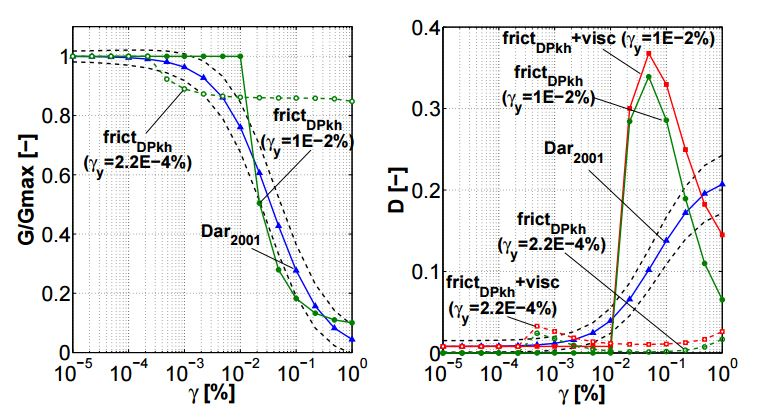
\includegraphics[width=0.9 \linewidth]{pisano}
	\caption{Comparison of a Drucker-Prager kinematic hardening bounding surface model (DPbs) with vanishing elastic region against Darendeli at $p_0=1 atm$. The results correspond to the work of Pisan\`{o},2014 \cite{pisano2014simulating}}
	\label{pisano}
\end{figure}

\begin{figure}[!h]
	\centering
	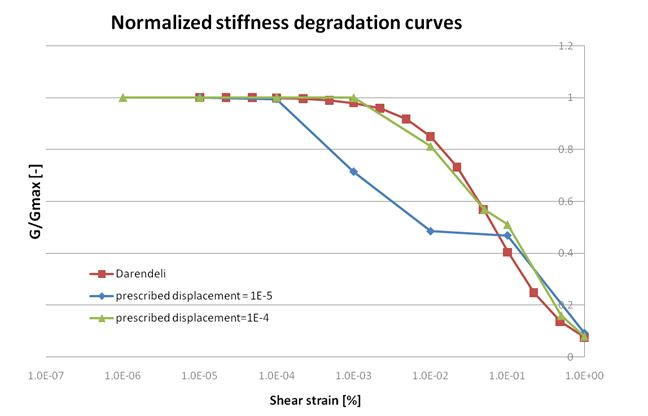
\includegraphics[width=0.9 \linewidth]{ggmax}
	\caption{Normalized stiffness degradation (right) and material damping (left) curves for various samples located along the soil layer depth. Comparison with the set of \mbox{normalized} curves proposed by Darendeli}
	\label{ggmaxi}
\end{figure}

%\begin{figure}[!h]
%\centering
%\begin{minipage}[b]{0.45\textwidth}
	%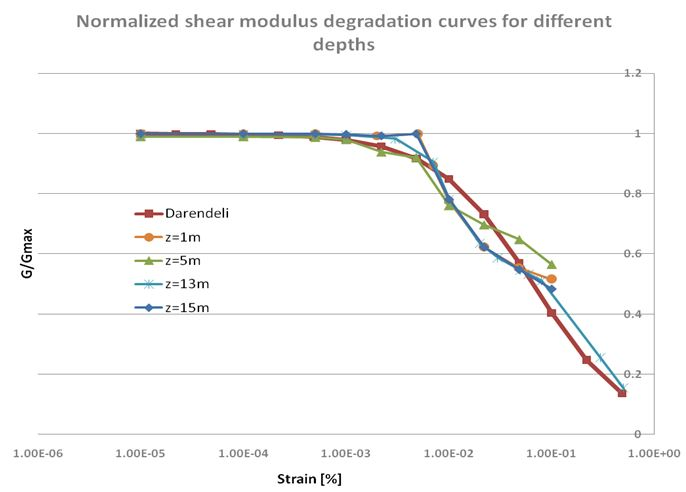
\includegraphics[width=\textwidth]{ggmax2}
	%\caption{Normalized stiffness degradation curves comparison}
	%\label{ggmax2}
%\end{minipage}
%\hfill
%\begin{minipage}[b]{0.45\textwidth}
%	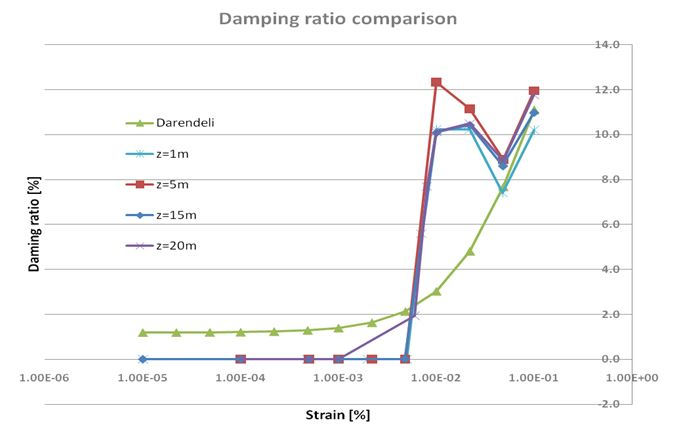
\includegraphics[width=\textwidth]{dampiing}
%	\caption{Damping ratio comparison}
%	\label{damping}
%\end{minipage}
%\end{figure}



\newpage
\section{Conclusions}
A strain-controlled numerical test was performed on a one element mesh assigned with properties corresponding to different clay samples located across the depth of a homogeneous layer. The test starts applying a vertical stress on the soil specimen for establishing the natural stress state. For the second step of the analysis, an uniform harmonic cyclic amplitude curve is defined and assigned to the lateral prescribed displacement $\gamma$ - this way, the cyclic loading is simulated. The values of the prescribed deformation varied from $10E^{-1}$ to $10E^{-6}$ in order to capture the small-strain domain. The investigation focuses on the influence of various parameters: the position of the sample within the soil medium, the strain level at which plasticity is triggered and lack of damping properties.

 The aim of the study strived to generate normalized stiffness degradation and material damping curves similar to the ones provided by Darendeli's, 2001 \cite{darendeli2001development}. They represent a reference standard in this domain, generated through a four-parameters mathematical model that describes the behaviour of a soil specimen when subjected to shear cyclic loading. It is suitable for dynamic problems that assist shear wave propagation - which is also the current case.

Despite the lack of damping parameters and coefficients that guarantee a smooth transition along the curvature, the model succeeds in generating the normalized modulus reduction curves and material damping with a decent degree of accuracy when examining in contrast with Darendeli's set of curves.  

It can be concluded that the proposed material model qualifies as reasonable for the future examination and, thus, the current paper continues the research towards a one-dimensional site response analysis. 

	\chapter {Site Response Analysis}
	\section{Introduction}
	The seismic waves generated at the bedrock suffer variation until they reach the surface; both the characteristics of the ground shaking as well as the material parameters influence the ground response that can be expressed in terms of amplitude, duration and frequency content. The importance of the ground response analysis relates to the overall dynamic study of the superstructure; the seismic waves can experience amplification or de-amplification at surface level as a function of soil damping properties together with encountered frequencies. In the case of matching frequencies between the maximum amplification of ground motion and natural frequency of the structure, the two elements (soil and construction) resonate one with the other. This translates into high \mbox{oscillating} amplitudes and thus, considerable damage. 
	
	In conclusion, performing a site response analysis enables the engineers to predict the site frequency content, the spectral acceleration alongside to peak ground acceleration and thus to create a reliable seismic design. Figure \label{Soilcolumn} presents the schematization of the entire site response analysis.
	
	
	\section{Model description}
	The model represents an extrapolation of the previous analysis step; the soil sample becomes a homogeneous layer with properties increasing linearly with depth and it is subjected to two steps: \textit{the gravity} and \textit{the seismic excitation}. The height of the layer is assumed 30 meters, have in mind it is merely an assumption - given the lack of bedrock and for the simplicity of calculation, the bedrock is considered located at 30m below surface. In order to simulate a one dimensional analysis, the problem is analysed in a 2D space plane strain ($\epsilon_{zz}=0$) with the lateral width of the soil relatively small compared to the height; the presence of bedrock translates into a rigid base having translational constraints in both directions and each pair of horizontal nodes are tied together such that will experience equivalent displacements. \label{fig:Soilcolumn} shows the schematization of the problem, the blue numbers representing the nodes, the red numbers the elements, respectively. The 1D soil column represents the typical model for a site response analysis as the shear wave propagation direction is assumed to be vertical - thus the main interest stands in the interaction between the soil profile and the vertically travelling seismic wave. 
	
	The validation of the model will consists of a result comparison between the analysis performed in Abaqus and the ones obtained from NERA together with the Groningen SRA performed by ARUP - the latter only offers a rough guide. The differences between the means of analysis will be investigated, the results will be expressed in terms of acceleration response in frequency domain together with stiffness degradation. 
	
	\subsection{Steps of analysis}
	The first step of the analysis simulates the natural stress state within the soil using a gravity load spread all over the layer and it is declared as static, general. The self weight of the elements provide the loads, therefore no need of extra loading conditions. The definition of the gravity load involves the software in updating several parameters to account for the confining pressure. As the schematization shows, the model contains elements and nodes - the nodes will be assigned with boundary conditions reproducing the one dimensional vertical propagation of the shear waves. The base nodes are constrained in both directions in accordance with the assumption of the bedrock presence underneath the soil layer whilst each pair of nodes horizontally displayed are linked using a feature called multi-point constraint - this provides a pinned joint between the nodes making the global displacements be equal leaving the rotations independent. 
	
	\begin{figure}
		\centering
		\includegraphics[width=0.7\linewidth]{"Soil column"}
		\caption[]{Schematization of soil column}
		\label{Soilcolumn}
	\end{figure}
	
	
	The second step represents the soil layer subjected to the earthquake motion; it is defined as a dynamic step calculated using an implicit integration scheme which will be explained in more detailed later on. During the step, the user propagates the boundary conditions aforementioned with the exception of the horizontal base constraint; it is replaced by an acceleration type of boundary condition that is assigned with an amplitude curve - this allows the user to define an arbitrary variation in time (or frequency) of any quantity or can be defined as a mathematical function (e.g. sinusoidal), series of values in time (acceleration history) and many more. For the current study, the amplitude curve contained the acceleration-time record for a period of 10 seconds as \ref{Acceleration} shows; this period is considered as the representative duration of Groningen acceleration measured time history and it starts right before the peak acceleration \cite{dost2004scaling}. By assigning the amplitude curve to the boundary condition on X direction together with a restraint in Y direction, the software converts this acceleration input to the base of the sample simulating the earthquake motion into relative force history acting on the model.
	
	\begin{figure}[h!]
		\centering
		\includegraphics[width=0.7\linewidth]{"Acc input"}
		\caption{Acceleration input (induced earthquake, @Huizige, 16 Aug 2012)}
		\label{Acceleration}
	\end{figure}
	
	\newpage
	\subsection{Input parameters}
	The material parameters, as presented in Chapter \ref{ch3} and Appendix \ref{App:AppendixB}, can be divided into several categories the software requires:
	\begin{enumerate}
		\item \textit{Elastic}\quad again, Young's modulus together with Poisson's ratio becomes sufficient for the definition of elastic domain.
		\item \textit{Plastic}\quad the nonlinear isotropic/kinematic model applies von Mises failure criterion for which three parameters are required: yield stress at zero plastic strain $\sigma_0$, small-strain Young's modulus $C$ and hardening parameter $K$.
		\item\textit{Density -}\quad the soil layer is considered to be homogeneous, thus one single material is define. So density for a silty-clay medium weak was considered 1800kg/m3
		\item \textit{Damping -}\quad the software offers many damping options [from numerical to material damping]; however, for this example the Rayleigh damping parameters $\alpha$ and $\beta$ are sufficient for the scope of analysis. This matter will be discussed later on.
	\end{enumerate}
	
	In addition, the model contains a subroutine which introduces the values of undrained shear strength as a function of the vertical effective stress as well as the correlation of this parameter with Young's modulus using field variables located at integration points of the elements. The field variable values can be functions of element variables such as stress or strain. Appendix \ref{App:AppendixG} shows the flow chart of Abaqus user defined subroutine together with the subroutine introduced in the calculation.
	
	The parameters are calculated as presented in the previous chapter (see Chapter \ref{ch3} and Appendix \ref{App:AppendixF}). One important matter to mention is the change in the calculation of Young's modulus - for the ease of calculation, this value was determined as a function of the undrained shear strength value. Anastasopoulos et al, 2011 \cite{anastasopoulos2011simplified} use an empirical formulae (based on e.g., Hardin and Richart, 1963 \cite{hardin1963elastic}; Robertson and Campanella, 1983 \cite{robertson1983interpretation}; Seed et al. 1986 \cite{seed1986use}; Mayne and Rix 1993) for calculating the value of the small-strain Young's modulus as a function of the overburden stress $\sigma_y$. $C=a{\sigma }_{y}$ with a ranging from 150 to 10.000 (for clays). Accounting for von Mises failure criterion and one of its defining equations ${\sigma}_{y}=a*S_u$ it finally yields:
	\begin{equation}
	E=a*S_u
	\end{equation}
	
	For this application, the value of a was considered to be a=2000 and the correlation between the measurements and empirically determined Young's modulus can be visualized in \ref{Young}
	
	\begin{figure}[h!]
		\centering
		\includegraphics[width=0.7\linewidth]{"Young's modulus"}
		\caption[]{Young's modulus distribution along depth}
		\label{Young}
	\end{figure}
	
	\subsection{Rayleigh coefficients}
	The dissipative character of the elasto-plastic material can be better enhanced by introducing a viscous damping mechanism. The overall stress state of the soil skeleton can be separated into two parts: 
	\begin{itemize}
		\item \textit{frictional component}- relating to the elasto-plastic behaviour, being displacement proportional
		\item \textit{viscous component} - relating to the Rayleigh damping coefficients, being velocity proportional. 
	\end{itemize}
	
	The advantage of coupling these two terms refers to the smoothing of the shear stress-strain cycles as well as a higher material damping. The viscous component has a favourable effect on the damping curves for small-strain domain; whilst it leads to an overestimation for large-strains. 
	As mentioned previously, the second step of the analysis, and the most important, is declared as dynamic, implicit. In non-linear analysis, the dynamic equation of motion is:
	\begin{equation}
	\left[M\right]{\Delta \ddot{u}}+\left[C\right]{\Delta \dot{u}}+\left[K\right]\Delta{u}=-\left[M\right]{I}\Delta\ddot{u}_g
	\end{equation}
	
	where [M] - mass matrix, [C] - viscous damping matrix, [K] - stiffness matrix, {ü},{ů} and {u} - vectors of nodal relative acceleration, velocity and displacement, üg - acceleration at the base and {I} - unit vector. The matrices are compiled based on the incremental response recorded within the software analysis. The equation is solved at every incremental time step using the Newmark method.
	
	The viscous damping matrix follows Rayleigh and Lindsay equation that relates the small strain damping to both mass and stiffness matrices. Thus, the equation for the viscous damping is:
	\begin{equation}
	\left[C\right]=\alpha\left[M\right]+\beta\left[K\right]
	\end{equation}
	where
	\begin{equation}
	\beta = 2\frac{\xi}{\omega_1}
	\end{equation}
	
	
	$\xi$ is the damping ratio at small strain; for this application $\xi$=1.2 corresponding to Darendeli's results; while $\omega_1$ is the natural circular frequency at first natural mode;
	
	The assumption of short layer leads to the simplification of the problem because the contribution of higher modes are relatively negligible. Despite that the experimental results prove that the damping matrix [C] is frequency independent and it has a constant value, Park and Hashash, 2002 \cite{hashash2002viscous} show the correlation between the stiffness [K] and the damping [C]. Since the stiffness depends on the strain level, then it can be concluded that the damping is also strain dependent, including the natural frequency. Thus, the viscous damping matrix [C] is updated at each time increment as well as the stiffness. Kramer proposes an equation for the calculation of the period of vibration that corresponds to the fundamental frequency of the selected mode as it follows:
	\begin{equation}
	T_n=(2n-1)\frac{\stackrel{-}{{V}_{s}}}{4H}\longrightarrow T_n=\frac{V_s}{4H}.
	\end{equation}
	
	where $\stackrel{-}{{V}_{s}}$ average shear wave velocity and H = layer height.
	
	Further, the natural circular frequency is obtained through the following transformation:
	\begin{equation}
	\omega_n=\frac{2\pi}{T_n} \rightarrow \omega_1=\pi\frac{V_s}{2H}
	\end{equation}
	
	And finally, Rayleigh $\beta$ damping parameter becomes:
	\begin{equation}
	\beta=\frac{2H\xi}{V_s\pi}
	\end{equation}
	
	\begin{table}[h!]
		\centering
		\begin{tabular}{|c|c|c|c|c|}
			\hline $\xi$         &       $1.2$    &  \%    &  Darendeli damping ratio      \\ 
			\hline $T_n$    & $4H/V_s$ &  sec &  Fundamental period\\ 
			\hline $V_s$  & 132  &  m/s &  Average shear wave velocity\\ 
			\hline $H$ & 30 &  meters &  Layer depth\\
			\hline $\omega$ & 6.91 & $Hz (sec^-1)$ & Fundamental frequency\\
			\hline $\beta$ & 0.001736 & sec & Rayleigh $\beta$ coefficient\\
			\hline
		\end{tabular} 
		\caption{Calculation of Rayleigh $\beta$ parameter}
		\label{beta_param}
	\end{table}
	
	\subsection{Integration scheme}
	It is important to understand the type of nonlinear analysis the software was opted to perform and its influence of the results. For this particular analysis, an implicit direct integration scheme was selected - this means that the set of nonlinear equations of motion solved at the time step $\Delta t_{n+1}$ are employed to compute the transition from the state at $t_n$ to $t_{n+1}$; on the other hand, an explicit integration uses all information at the beginning of $t_n$ to estimate the latter state at $t_{n+1}$.
	
	Abaqus/Standard uses the Hilber-Hughes-Taylor time integration method \cite{hilber1977improved} which is an extension of the Newmark $\beta$ method, 1959 \cite{newmark1959method}. Basically it controls the numerical damping within the system which might rise due to the energy dissipation mechanisms associated with different operator types. More details related to Newmark integration method are presented in Appendix \ref{App:AppendixH}.
	
	\subsection{FEM stability}
	According to Jeremi\'{c}, \cite{jeremic2009time}, the accuracy of such nonlinear problem dealing with wave propagation is controlled by two factors - node spacing in the FE model $\delta h$ and the time step $\delta t$. The spacing is directly related to the wavelength whilst the time step depends on the fundamental period of the system. 
	\begin{equation}
	\Delta h\leq\frac{\lambda_{min}}{10}=\frac{1}{10} \frac{v}{f_{max}}
	\end{equation}
	
	\begin{equation}
	\Delta t=\frac{T_n}{10}
	\end{equation}
	More details regarding the calculation of the two stability criterion are presented within Appendix \ref{App:AppendixI}
	
	\subsection{Mesh}
	For the mesh elements, four-node quad elements ($CPE4$) are used to model the soil using the plane strain formulation of the quad-element. The element connectivity uses a counterclockwise pattern for the previously-described node numbering scheme (see \ref{Figure 1}). The soil elements in each layer are assigned the material tag of the material object corresponding to that layer. A unit thickness is used in all examples for simulating the 1D condition. The self-weight of the soil is considered as a body force acting on each element. The body force is set as the unit weight of the soil in each layer, which is determined from the respective mass density input value.
	
	
	\section{NERA - Non-linear Earthquake Site Response}
	An additional analysis was performed using NERA (Nonlinear Earthquake site Response Analyses) computer program in order to have a better grasp of the whole concept as well as a meaningful comparison. It derives from EERA that uses an equivalent linear model to investigate the same problem; the constitutive material model is proposed by Iwan and Mroz, 1967 \cite{mroz1967description} and it describes the nonlinear kinematic model as a series of n mechanical elements, each displaying different stiffness ki and sliding resistance $R_i$ as it is shown in \ref{Mroz}. More details concerning the calibration NERA performs are presented in Appendix .
	
	\begin{figure}[h!]
		\centering
		\includegraphics[width=0.7\linewidth]{"Mroz"}
		\caption[]{Plasticity description of Iwan and Mroz nonlinear model}
		\label{Mroz}
	\end{figure}
	
	NERA is composed by a FORTRAN 90 code together with a Excel plug-in that capture the nonlinear site response of a layered soil column subjected to an earthquake signal. As input, it requires the acceleration-time record, elastic material properties with emphasis on the stiffness parameters - normalized stiffness degradation and material damping curves. 
	
	The material properties introduced within the software require a general description of the soil column as well as an individual material classification (in case the user is dealing with a multi-layered ground). The general input portrays the column with its sub-layers and unit weights, shear wave velocities and the ground water table followed by an automatic assessment of the maximum shear modulus, effective stresses and fundamental period. 
	
	The software allows for multiple layer definition by introducing the normalized shear modulus degradation curves and material damping curves. For this particular case, Darendeli's results presented previously were used in order to obtain a consequent comparison. However, the software does not account for data corresponding to damping curves as it is calculating its own set of values. This is because the nonlinear model proposed by Iwan and Mroz uses a different scheme for determining the damping characteristics.
	
	NERA starts the analysis by processing the earthquake input signal and material properties followed by step-by-step determination of the relative velocity and displacement at a selected sub-layer. The integration scheme NERA uses is the central difference which, contrary to Abaqus analysis, it is conditionally stable (the time step size is limited). This calculation method is a particular type of Newmark method in which the predicted velocity is:
	
	\begin{equation}
	\tilde{v}_{i,n+1}=v_{i,n}+\frac{1}{2}a_{i,n}\Delta t
	\end{equation}
	
	The stress and strains are calculated at each node from nodal displacements, next step calculates the velocity from the input acceleration history. Subsequently, the predicted values for velocities at time $t_{n+1}$ yield from those determined at time $t_n$ and finally the nodal displacements, velocities and accelerations are update at each node i. In addition, the output includes spectral response based on Fourier transform calculation for any selected sub-layer.
	
	\section{Results}
	This subchapter presents the results obtained from the site response analysis performed in Abaqus, followed by a comparison with NERA outcome; several plots are used as mean of verification and the main interest lies on the $G/G_{max}$ and damping curves, acceleration response as well as the amplification ratio in frequency domain.
	
	After performing a dynamic, implicit type of analysis to the assembly described previously, the output was investigated with an initial emphasis on the stiffness degradation. To check the validity of the overall model, an uniform cyclic signal served as acceleration amplitude; a circular frequency $f=1 Hz$ was applied at the bottom of the model for a period of 10 seconds in a sinusoidal fashion. Such uniform harmonic loading represents a simplification of the signal, and helps the user better understand the non-linear soil response. A real acceleration-time history consists in many irregularities and the results may be sometimes misinterpreted. That is why the investigation starts simple towards complicated.
	
	The results can be visualized in \ref{response1}, \ref{response2} and \ref{acc1}. The same remarks can be made as for the preceding analysis (see previous analysis in Chapter \ref{ch3}); however, this model includes an additional Rayleigh damping parameter together with the subroutine that updates the values of the Young's modulus. The acceleration response displays a de-amplification of the bottom signal together with damping effects visible in the irregularities of the curves; the de-amplification effect can be seen as the average wave speed decreases (blue line wave travels with 0.5m/s whilst the green line with almost half the speed). The values are obtained by dividing the maximum acceleration to the time period of a complete sinusoidal cycle. The shear stress-strain plots show plasticity occurring at different stress levels - the hysteresis loops shift towards origin which means that the soil achieves plasticity gradually. Additionally, the plots show a decrease in dissipated energy as the seismic waves travels from bottom to top - the area comprised within the hysteresis loops reduces as well.
	
	%introduce the soil column picture
	\begin{figure}[h!]
		\centering
		\includegraphics[width=0.7\linewidth]{"response1"}
		\caption[]{Hysteresis loops on the lower half of the soil layer (Element 1 - Base; Element 15 - Middle of the layer)}
		\label{response1}
	\end{figure}
	
	\begin{figure}[h!]
		\centering
		\includegraphics[width=0.7\linewidth]{"response2"}
		\caption[]{Hysteresis loops for lower half of the soil layer(Element 1 - Base; Element 31 - Surface)}
		\label{response2}
	\end{figure}
	
	\begin{figure}[h!]
		\centering
		\includegraphics[width=0.7\linewidth]{"acc_response1"}
		\caption{Acceleration response (surface and bottom)}
		\label{acc1}
	\end{figure}
	
	Going forward with the results, the real acceleration-time history was applied to the boundary condition at the bottom nodes for the same period of 10 seconds. The records correspond to the measurements from WSE station, Huizinge, Groningen \cite{dost2013august} - even though the earthquake signal lasts for 35 seconds, it was trimmed to analyse the most unfavourable 10 seconds [with the highest acceleration peak]. The obtained values in terms of shear stress and strain can be seen in \ref{resp3} whilst the top and bottom acceleration outcome is represented in \ref{acc_resp2}. Important to mention is that the boundary condition applied at the bottom of the model represents the bedrock presence, therefore the waves are incident and not reflective - the discussion about the boundary conditions influence on the wave propagation shall be presented shortly after. [As a sign convention, element 1 represents the bottom one whilst element 30 is the surface].
	\begin{figure} [h!]
		\centering
		\includegraphics[width=0.7\linewidth]{"response3"}
		\caption{Hysteresis loops for upper half of the layer when real acceleration is applied}
		\label{resp3}
	\end{figure}
	
	\begin{figure}[h!]
		\centering
		\includegraphics[width=0.7\linewidth]{"acc_response2"}
		\caption{Acceleration response - surface and bottom}
		\label{acc_resp2}
	\end{figure}
	%introdu citat
	Once the bottom and top acceleration outcome is extracted from the software, a Fast Fourier transform is applied with the scope of converting the current data from time domain to a representation in frequency domain. As Kristeková et al., 2006 \cite{kristekova2006misfit} stated "the most complete and informative characterization of a signal can be obtained by its decomposition in the time-frequency plane". However, FFT is used as a digital signal processing tool that aids other operation, rather than providing a final result itself. For example, the transfer function or a site amplification factor allows the calculation of the motion of any layer $i$ based on other motion (of any layer $j$). This transfer function relates the displacement at position $i$ to that at position $j$ as it follows:
	\begin{equation}
	F_{ij}=\frac{|u_i|}{|u_j|}
	\end{equation}
	
	The Fourier spectrum represents the distribution of energy in the ground motion for a frequency interval $[0 ≤ f ≤ 1/2\delta t]$. The amplification factor can also be written as:
	\begin{equation}
	A(f)=\frac{F_{a,site}(f)}{F_{a,bedrock}(f)}
	\end{equation}
	where $A(f)$ - site amplification factor; $F_a,site(f)$ and $F_a,berock(f)$ - Fourier amplitudes of ground acceleration at surface and bedrock, respectively calculated as the vector sum of the two horizontal components. The importance of the site amplification factor relates to the structural damage pattern (rather than the PGA amplification) due to site effects. If the natural period of the structure matches the soil natural period, the structure will be more vulnerable to earthquakes. 
	\begin{figure}[h!]
		\centering
		\includegraphics[width=0.7\linewidth]{"Fourier"}
		\caption{Fourier amplitude spectra - surface and bottom}
		\label{fourier}
	\end{figure}
	%alta referinta Zienkiewicz
	It is important to discuss the boundary conditions and their influence on the wave transmission throughout the layer. The current model created in Abaqus includes tied boundaries, also described by Zienkiewicz et al. (1989) \cite{zienkiewicz1989earthquake} and it assumes that all displacements on the left side of the column correspond to the ones at the right side, simulating a free field boundaries, whereas the bottom nodes do not absorb the oscillating waves. The software offers the baseline correction option for the acceleration input for time domain analysis; the practice is proposed by Newmark \cite{newmark1959method} and it introduces an additional correction to the acceleration such that the mean square velocity over the event time is minimized. The use of more correction intervals provides tighter control over any “drift” in the displacement at the expense of more modification of the given acceleration trace. However, in acceleration history it does not show large difference between the responses.
	
	Because the boundary only transmits the waves upwards, an additional analysis was performed with a bottom acceleration record manually reduced by half. Physically, the waves within a soil have both downwards and upwards motion (incident and reflective). The decision of applying half of the signal also relates to NERA calculation in order to obtain a coherence between the two software; NERA assumes that the velocity at base is the sum of both incident and reflected waves and since at bedrock level shear force is zero it yields that the velocity becomes:
	
	\begin{equation}
	v_{base}=2v_{incident}
	\end{equation} 
	
	\section{Comparison Abaqus vs NERA}
	The comparison between the two analyses were formulated in terms of acceleration response, shear stress-strain response together with the spectral ratio and the plots can be visualized below. 
	
	\begin{figure}[h!]
		\centering
		\includegraphics[width=0.7\linewidth]{"acc_response2"}
		\caption{Acceleration comparison Abaqus vs. NERA}
		\label{comp1}
	\end{figure}
	
	\begin{figure}[h!]
		\centering
		\includegraphics[width=0.7\linewidth]{"spectral2"}
		\caption{Fourier amplitude spectra comparison}
		\label{fourier2}
	\end{figure}
	
	\begin{figure}[h!]
		\centering
		\includegraphics[width=0.7\linewidth]{"tau_gamma1"}
		\caption{Hysteresis loops comparison for surface level}
		\label{tau_gamma1}
	\end{figure}
	
	\begin{figure}[h!]
		\centering
		\includegraphics[width=0.7\linewidth]{"tau_gamma2"}
		\caption{Hysteresis loops comparison for z=20m(left) and bottom level(right)}
		\label{tau_gamma2}
	\end{figure}
	
	\subsection{Remarks}
	It is difficult to have a relevant comparison at surface level when the sample experiences low stresses; calibration of cyclic parameters was referred to considerably higher confining stresses. Moreover, it was noticed that Abaqus generates higher plastic strains; this might explain the signal attenuation expressed in frequency domain when comparing to NERA response. 
	
	Overall, the results show a quite satisfying match; nonetheless, differences appear due to several factors as it follows:
	\begin{enumerate}
		\item Abaqus works with a dynamic implicit integration scheme with an Euler backwards theory that is unconditionally stable whereas NERA solves the system of equation through a central-difference which is conditionally stable; thus on one software, user has the option of manually adjusting the time step while on the other he cannot. The equation of motion for the system in dynamic domain it is basically the same:
		\begin{equation}
		f=F-\rho\ddot{u}
		\end{equation}
		where f - body force, F - external body force, $\rho$ - soil unit weight and $\ddot{u}$ - relative nodal acceleration. Thus, the difference is \textit{numerical} and cannot be adjusted in detail.
		\item Both the models are based on the concept of a yield surface which means that there is a surface defined in stress space within which no plastic deformation takes place. The nonlinear kinematic hardening model used in Abaqus is based on the Lemaitre and Chaboche model that considers two yield surfaces and a varying hardening modulus whilst NERA works according to Iwan and Mroz multi-linear kinematic hardening model that has a multiple surface plasticity. First model includes a 'fading memory' term whereas the second model does not and preserves the memory width. Thus, the difference is related to the plastic domain and how the model behaves when irreversible deformations are encountered. 
		\begin{figure}
			\centering
			\includegraphics[width=0.7\linewidth]{"yield_srf"}
			\caption{Non-linear kinematic hardening model according to Lemaitre,Chaboche [left] and Iwan,Mroz[right]}
			\label{Yield}
		\end{figure}
		\item NERA computes the shear stress and strain increments according to the sliding resistance and tangent modulus of each slider that are derived from the $G_i-\gamma_i$ points introduced as input. The tangential shear modulus is related to the secant shear modulus by $H_i=G_{max}\frac{G'_{i+1}\gamma_{i+1}-G'_i\gamma_i}{\gamma_{i+1}-\gamma_i}$ where $G_i=\frac{G_i}{G_{max}}$ . The stiffness of each component of the system is related to the tangent modulus while the shear stress is associated with the sliding resistance. On the other hand, Abaqus does not work with the tangent modulus, but with maximum shear modulus Gmax and the undrained shear strength. Also, in NERA there is no option for introducing the values corresponding to the undrained shear strength or its correlation with any other parameter. Figure 14 shows the distribution of the shear modulus with depth in both the software - these values are calculated from the input parameter - Abaqus extracts it based on the Young's modulus together with Poisson's ratio whilst NERA does it based on the soil unit weight and shear wave velocity. The values are exactly the same, it can be noticed also from the slope the hysteresis loops presented in the stress-strain plots; the width also resembles as well as the unloading-reloading areas. However, the tangent shear modulus differs from one software to the other.
		\begin{figure}[h!]
			\centering
			\includegraphics[width=0.7\linewidth]{"shear"}
			\caption{Shear modulus $G_{max}$ comparison}
			\label{shear1}
		\end{figure}
		\item Abaqus results are extracted in two different locations: the stresses and strains are obtained from Gauss integration points and the accelerations are obtained at nodal positions which are situated at the interface of each two element. NERA performs the analysis according to the middle of each sub-layer, so both the top and bottom outcome are actually 0.25m below the surface or above the bottom. However, not much difference should rise from this aspect.
		\item Another difference relates to the viscous part of the model and it is more apparent in the acceleration response in time domain, especially in the initial period. Abaqus works with the viscous term defined exclusively as a function of Rayleigh damping parameter $\beta$ meaning that the system damping depends on the stiffness, whilst NERA requires the critical damping ratio value, incorporating both $\alpha$ and $\beta$ Rayleigh factors. Moreover, the energy dissipation mechanism accounts for both viscous damping and plasticity terms which, as described previously, differ from NERA to Abaqus. When working with a high PGA value, the contribution of the non-linear model and hysteretic damping becomes greater compared to the viscous damping component.
		\item The aforementioned differences between the calculation programs derive mainly from numerical algorithms; however, a more important aspect seems to govern the outcome of each analysis - the dynamic nature of the problem itself. The two models are not identical, thus a difference in any given point might generate distinct response at unknown location and time because of the non-linear propagation fashion. 
		\item Noise can be experienced in both the signals of the different computer programs. This can distort the final results; filtering is possible, however it is time demanding and does not represent the main interest in this study.
	\end{enumerate}
	
	\subsection{Additional investigation}
	An additional investigation was performed in order to check the soil response when closer to elastic domain - as in, a lower PGA was applied at the bottom boundary. The first analysis contained a PGA value of approximately 0.5g whilst the second one scaled down the value to 0.1g. The results can be seen in the following figures.
	
	\begin{figure}[h!]
		\centering
		\includegraphics[width=0.7\linewidth]{"acc_low"}
		\caption{Acceleration response comparison for PGA=0.1g}
		\label{acc_low}
	\end{figure}
	
	\begin{figure}[h!]
		\centering
		\includegraphics[width=0.7\linewidth]{"hysteresis_low_bot"}
		\caption{Hysteresis loops comparison for bottom level}
		\label{hyst_bot}
	\end{figure}
	
	\begin{figure}[h!]
		\centering
		\includegraphics[width=0.7\linewidth]{"hysteresis_low_surf"}
		\caption{Hysteresis loops comparison for surface level}
		\label{hyst_top}
	\end{figure}
	
	\begin{figure}[h!]
		\centering
		\includegraphics[width=0.7\linewidth]{"spectral_low"}
		\caption{Fourier amplitude spectra for PGA=0.1 - logarithmic scale}
		\label{fourier3}
	\end{figure}
	
	\begin{figure}[h!]
		\centering
		\includegraphics[width=0.7\linewidth]{"spectral2"}
		\caption{Site amplification factor comparison for PGA=0.1g}
		\label{SAF}
	\end{figure}
	\begin{figure}[h!]
		\centering
		\includegraphics[width=0.7\linewidth]{"ARUP"}
		\caption{Groningen site non-linear ground response, input vs surface PGA according to ARUP report}
		\label{ARUP}
	\end{figure}
	
	The results confirm the expectation regarding the amplification effect of the soil combined with the PGA level, also they are in accordance with ARUP report regarding the site response analysis performed for the specific location in discussion. The acceleration responses at surface produced in both the computational software present the same maximum value, of course, with differences that were exposed previously, the elastic response seems to match together with the stiffness degradation effect. 
	
	\section{Conclusions}
	The differences between the software were investigated and speculated; given the fact that the study deals with a non-linear kinematic hardening process, it becomes quite difficult to point exactly the main cause that leads to dissimilarity. However, reasons can be examined and despite the analyses run according to separate models and integration schemes, overall they display a reasonably agreement.
	
	It can be concluded that for the Groningen sites, low PGA input ($a_g=0.1g$) the surface acceleration response amplified whereas when dealing with a high PGA input ($a_g\textgreater0.15g$) the top PGA is de-amplified. Both the strength properties of the homogeneous medium and the earthquake motion characteristics influence the seismic wave propagation though the soil; for this particular case, the inelastic response depends on the limited capability of the soft layers to transmit seismic signals to the surface because of the low strength and on the high hysteretic damping observed at large strains. At low PGA values, the soil displays elastic behaviour as it reaches the surface, the frequencies do not experience considerable damping whereas at high PGA levels, the soil shifts towards its natural frequency, damping the higher ones and non-linear constitutive model plays a more important role than the viscous damping effect.
	\chapter{Soil Structure Interaction analysis} \label{ch6}
	
	The current chapter presents the analysis performed in 2D plane stress domain of the soil-footing(-structure) interaction when subjected to a recorded acceleration-time history. Various methods of seismic implementation are carried out to examine aspects such as load effects on soil response, effectiveness of energy dissipation mechanisms and the occurrence of foundation uplift.
	
	\section{New design philosophy}
	As previously presented, the new design philosophy suggests a different perspective on the induced non-linearity over the soil-structure assembly. Researchers involved within this study (Anastasopoulos et al., 2010 \cite{anastasopoulos2010soil}, Gazetas et al, 2013 \cite{gazetas2013nonlinear}, Apostolou et al., 2011 \cite{apostolou2011soil}, etc.) showed \mbox{several} effects associated with soil "failure" as acting beneficially in case of seismic ground motion. The interest in the present essay is to apply such approach on a different setting: soft soils, lack of bedrock, induced, and not tectonic, earthquakes together with shallow foundations. In order to summarize the goals, it is utmost important to define the characteristic non-linear effects:
	\begin{itemize}
		\item separation at soil-footing surface under rocking vibration also known as \textit{uplifting} that occurs when negligible interface tensile capacity is considered.
		\item mobilisation of the bearing capacity type of failure mechanism  when experiencing large cyclic overturning moments - \textit{soil failure}.
		\item plastification of the underlying ground in the proximity of the edges of the foundation \mbox{induced} by large vertical stresses.
	\end{itemize} 
	
	\section{Problem definition}
	The former chapter gets extended towards a 2D plane stress problem involving a soft soil layer supporting a shallow foundation. The entire structural system is subjected to a seismic input motion. The study aims at inspecting the inelastic soil response, the proposed method accuracy and its limitations. The final goal is to be able to acknowledge the new design philosophy suitability for this specific earthquake in Groningen area.
	
	\section{Model description}
	The object of study of the current chapter includes a soil layer of 30 meters deep together with a simplified soil-structure system resting upon it. As expected, the soil properties do not change drastically, for all the work that was previously conducted proves the parameters validity. Thus, the preceding model (1D soil column, see chapter 4, section 4.2.2) is expanded into a larger soil layer supporting the shallow foundation. A chimney located in Hoogezand village, Groningen, in  the north of Netherlands serves as example for the building and it was chosen for its relatively simple geometry together with available structural properties. The location and the chimney itself can be seen in Figures \ref{Boom} and \ref{chimney}.
	
	\begin{figure}[!h]
		\centering
		\includegraphics[width=0.5 \linewidth]{"Boomgaard"}
		\caption{Map location of the chimney - Groningen area}
		\label{Boom}
	\end{figure} 
	
	\begin{figure}[!h]
		\centering
		\includegraphics[width=0.5 \linewidth]{"chimney"}
		\caption{Real structure objected to study}
		\label{chimney}
	\end{figure} 

	
\section{Method of analysis}
The inelastic soil response investigation is implemented numerically with a finite element model considering two-dimensional plane strain assumptions. Both soil medium and \mbox{footing} are modelled as deformable solids using quadrilateral, continuum elements. The chimney is represented by a rectangular footing with a lumped mass on top of a slender, rigid pier. Moreover, the footing is also considered to behave in a stiff fashion when seismically loaded. The main emphasis is on the soil response rather than on the structural one, thus the simplification. A state-of-art contact algorithm defines the soil-structure interface incorporating uplifting and sliding features whereas purely elastic impact assumption is adopted. Every analysis starts with a \textit{static step} - the geostatic step in which initial stress conditions are established.  

The dynamic analyses operate through an implicit direct-integration algorithm - the global set of non-linear equations of motion is integrated in time domain via the implicit Hilber-Hughes-Taylor operator (a customed Newmark's method). As it was mentioned before, the Newmark's method includes the $\alpha$ and $\beta$ parameters with the values explained in the previous chapter (see section 4.2.4, chapter \ref{ch3} and Appendix \ref{App:AppendixH}). The numerical stability is achieved by calibrating both the mesh size and the time-step increment in such a way that elastic wave propagation laws are not violated; the calibration is also explained in Appendix \ref{App:AppendixI}. A schematization of the FE model can be seen in Figure \ref{mainM} followed by a detailed description of the model.

\subsection{Analysis procedure}
The research strategy resembles to the ones previously presented (see section 4.2.1). Each analysis begins with a geostatic step such that the in-situ stresses are established first. Gravity load is applied all over the soil medium, simulating the real soil status when no foundation is resting on the ground.

Further on, the footing influence is similarly introduced as the material density together with the gravity load define the foundation self weight. No additional vertical load is required so far. Moreover, the rigid pier includes a mass element at the top that simulates the superstructure weight. In the end, the whole assembly aims to reproduce a single-DOF structure.

Lastly, the seismic excitation must be integrated within the model. In order to get a smooth transition from the Site Response Analysis (SRA) towards the final goal, the study first assumes an sinusoidal cyclic input at the base of the soil layer. Finally, the real acceleration time history presented in previous chapter serves as example. The PGA is assumed to be 0.28g and it is implemented at a depth of 30 meters. Firstly, because this location is consistent with the SRA performed in chapter 4 and secondly, because it simulates the presence of bedrock.

The boundary conditions are formulated such that it accounts for seismic wave propagation and reflection at the bounds. Numerical stability, computational expenses and model dimensions play an important role for the accuracy of the output and require most attention.  %Henceforth, different types of boundary conditions were imposed that mimic the acceleration time history in distinct manners. Important to keep in mind that some methods do not necessarily require dynamic algorithms, a quasi-static analysis is preferable for such cases - this aspects will be explained in detail later in this chapter.

Thus, there are three main steps conducted within all analyses:
\begin{enumerate}
	\item \textbf{Geostatic} - for setting up the initial stress conditions of a free-field;
	\item \textbf{Self weight application} - representing the perturbation on the stresses close to the surface due to the presence of the footing;
	\item \textbf{Dynamic/ Quasi-static} - applying the seismic input in various manners to simulate the earthquake motion.
\end{enumerate}

\subsection{Contact definition}
An important role in triggering uplifting is played by the contact definition. The user can create and customize the interface properties according to the desired application. In finite element analysis, contact conditions describe a particular category of discontinuities, enabling forces to be transmitted from one part to another. The model must recognize and distinguish when the parts are in contact and when separation occurs in order to apply the constraints properly. 

Abaqus offers the possibility of defining contact pairs or contact elements; the former is recommended and it is based on the master-slave formulation. In addition, it allows the definition of these entities as surfaces or a collection of nodes - the differences refer to methods of discretization and calculation. In order to define a contact, its interaction properties have to be formulated first. Again, Abaqus allows the user to customize these features in correspondence with the model in use. For this particular case, only mechanical properties were created. An advanced contact algorithm is applied in order to permit uplifting and sliding and, additionally, to control their development during the seismic excitation. 

As previously mentioned, the study investigates two types of soil-footing contact: \textit{fully bonded} and \textit{tensionless sliding interface}. The advanced algorithm referes to the sliding interface whilst the fully bonded contact is effortlessly depicted through a \textbf{Tie constraint} - using the same master-slave formulation, it provides a simple way of bounding the two surfaces permanently, preventing sliding/separation.

However, the tensionless sliding interface requires much more attention and research as it incorporates various features that will be detailed further on.
 
\paragraph{Mechanical properties}   
The contact is described for both normal and tangential direction, more precisely a pressure-overclosure relationship illustrates the normal behaviour whereas a frictional interaction deals with the tangential behaviour. 

For normal direction, Abaqus implements a "hard-contact" relationship by default which consists of:
\begin{itemize}
	\item no penetration of master surface into the slave;
	\item no upper bound for the transmitted contact pressure;
	\item no stress transfer between surfaces when there is no contact detected.
\end{itemize}

Nonetheless, the current study indicates another type of normal contact, a softened one involving a pressure-overclosure relationship. According to Abaqus documentation, the softened contact can be introduced as linear or exponential, the latter being preferred. In an exponential (soft) contact pressure-overclosure relationship the surfaces begin to transmit contact pressure once the clearance between them, measured in the contact (normal) direction, reduces to $c_0$. The contact pressure transmitted between the surfaces then increases exponentially as the clearance continues to diminish. The schematization of the relationship can be visualized in Figure \ref{pressure}.
\begin{figure}[!h]
	\centering
	\includegraphics[width=0.45 \linewidth]{"pressure"}
	\caption{Exponential “softened” pressure-overclosure relationship in Abaqus/Standard}
	\label{pressure}
\end{figure} 

where \gls{p0} is the contact pressure at zero distance, \gls{c0} is the distance from the master surface at which the pressure is decreased to 1 \% of $ p_0$. The behaviour in between is exponential. A large value of $ c_0$ leads to soft contact, a small value to hard contact. It is difficult to know a priori which values are suitable, however literature studies suggest for $p_0=10 kPA$ correlated with a clearance $c_0=10E^{-5} m$.


For the tangential behaviour, the software provides the following options:
\begin{itemize}
	\item frictionless - default;
	\item rough - no slip is allowed;
	\item penalty friction which allows for:
		\begin{itemize}
			\item Coulomb friction law $T=\mu N$;
			\item constant shear limit at surface;
			\item friction coefficient as a function of the slip rate and contact pressure;
		\end{itemize}
\end{itemize}

Considering the cohesive character of the soil, the Coulomb friction law might not be the appropriate solution, thus the second option was chosen. This shear stress limit is typically introduced in cases when the contact pressure stress may become very large causing the Coulomb theory to provide a critical shear stress at the interface that exceeds the yield stress in the material beneath the contact surface. A reasonable upper bound estimate for $\tau_{max}$ is $\sigma_y/\sqrt{3}$, where $\sigma_y$ is the Mises yield stress of the material adjacent to the surface. In some cases some incremental slip may occur even though the friction model determines that the current frictional state is “sticking.” In other words, the slope of the shear (frictional) stress versus total slip relationship may be finite while in the “sticking” state, as shown in Figure \ref{stick}.

\begin{figure}[!h]
	\centering
	\includegraphics[width=0.5\linewidth]{"stick"}
	\caption{Elastic slip versus shear traction relationship for sticking and slipping friction}
	\label{stick}
\end{figure} 

The relationship shown in this figure is analogous to elastic-plastic material behavior without hardening: K corresponds to Young's modulus, and $\tau_{crit}$ corresponds to yield stress; sticking friction is associated with the elastic regime, and slipping friction to the plastic one. A typical average value recommended in the literature for the elastic slip is 0.1mm and it seems appropriate for this case as well.

\paragraph{Contact interface discretization}
Having defined all interaction properties, the contact itself must be formulated; the most suitable interaction option Abaqus/Standard offers is \textit{Surface-to-surface}; the contact discretization can be chosen node-to-surface (N-S) or surface-to-surface (S-S), the latter being preferable. Firstly, because the conditions will be enforced based on an average region instead of strictly node-wise. The averaging regions are approximately centred on slave nodes, so each contact constraint will predominantly consider one slave node but adjacent slave nodes. Secondly, this option does not include spikes in the pressure distribution along the surface, as it happens in the N-S case. Lastly, large and unintended penetration of master nodes into slave does not occur leading to a smoothing effect.

The sliding formulation required for the interaction implementation has two options as well: finite sliding or small sliding. The second alternative is more convenient, as the footing will not slide considerably. Moreover, coupling of slave nodes with their projections on master surface is calculated at the beginning of the analysis and does not change throughout the analysis, whereas for finite sliding approach, this coupling is checked and recalculated throughout the analysis.

\subsection{Boundary conditions}
The first set of BCs refers to the soil layer and it assumes the top surface as being constraint-free, whilst rigid bottom is initially defined. The lateral boundaries are both vertically and horizontally constrained. The structure (SDOF) resembles to a cantilever, the base (footing) is connected to the soil via the contact algorithm (fixed end) while the top of the pier is allowed to translate and rotate (free end).

Nevertheless, in dynamic analyses, a fixed boundary condition will lead to wave reflection at the outer limits of the model which means energy trapped inside the model. This effect becomes detrimental, therefore solutions must mitigate reflective waves propagating throughout the model. One way is to create a large enough soil body to simulate an infinite medium. Another concept relates to transmitting boundaries and many researchers proposed methods of tackling the problem, here highlighting the work of Lysmer and Kuhlemeyer, 1969 \cite{lysmer1969finite} and Zienkiewicz et al (1989) \cite{zienkiewicz1989earthquake}.

However, for simplicity of the problem, these complex concepts were not implemented so the focus was on verifying the accurate position of the lateral boundaries. Moreover, the current application is dealing with a simple geometry, reduced  footing-structure dimensions and a dissipative material. So it can be assumed that soil plasticity will favour the energy dissipation and prevent the wave reflection at lateral boundaries to greatly influence the response in the proximity of the foundation.

 \paragraph{Tied lateral boundaries}
	The traditional approach considers pairs of lateral nodes being tied together such way that the horizontal and vertical displacement are equal throughout the entire analysis. This feature can be easily achieved using Abaqus MPC (multi-point constraint) option specifically designed for this situation. The assumption is in conformity with Zienkiewicz's work (\cite{zienkiewicz1989earthquake}) stating that the presence of the structure on soil oscillation is negligible when the boundaries are sufficiently far.
	
	Subsequently, the input motion is introduced at the vertically fixed base of the model that replicates the presence of the bedrock. As previously discussed, the acceleration signal obtained from the dataset for Groningen field was recorded at borehole depth, not at bedrock, which means that the recordings can include both incident and reflected waves. In order to exclude an overestimation of the real input signal, the accelerogram was truncated in half to ensure that only upward travelling waves are considered.
	
	Nevertheless, this method can be formulated in the FE product either through a dynamic or a quasi-static step depending whether the earthquake is expressed in terms of total displacements or total accelerations.
	
	However attractive this simple method might be, its shortcomings originate from both the lack of an actual bedrock or from the uncertainties rising when defining the model dimensions - there are no rule of thumbs for determining the truncation of the mathematical model. Thus, in order to establish a correct location for these boundaries, various tests were performed introducing the concept of free-field soil column.
	
	\paragraph{Free-field soil column}
	It behaves similarly to a vertical soil medium located far enough from the actual foundation for the vibrations not to perturb its state stress. This can be simply implemented as the one-dimensional column subjected to seismic excitation, identical to the model created for the site response analysis. Its advantages involve the option of extracting the results at any desired node. Thus, the previous analysis becomes essential as it represents the benchmark when verifying the soil medium dimensions.
		
	It is worth to acknowledge the constraints which link pairs of lateral nodes in order to maintain equal horizontal displacements along the seismic test. Then, it suffices extracting the outcome from one set of lateral nodes, since left or right are displaying equal results. The output yields displacement, velocity and acceleration time histories for each lateral node - allowing the comparison with the main model lateral response.
			
	A series of results extracted from the SRA are presented below:
		\begin{figure}[h!]
			\centering
			\includegraphics[width=0.8\linewidth]{"response_model_v12_FBC"}
			\caption{Acceleration, velocity and displacement time histories output throughout the free-field soil column}
			\label{Acc_ff}
		\end{figure} 
		
	Once the response at the lateral boundaries of the main model corresponds to the one recorded from the free-field soil column, then the location of the boundaries becomes valid and the final dimension of the model can be established. For this particular case, it was concluded that a total length of the soil medium, L=100m, is sufficient to incorporate both near and far field domains. Figure \ref{validation}) shows a comparison between the response obtained from both one-dimensional model and the main 2D model.
		\begin{figure}[!h]
			\centering
			\includegraphics[width=0.7\linewidth]{"free-field2"}
			\caption{Validation for soil layer width by comparing the acceleration response at surface level}
			\label{validation}
		\end{figure}			
			
			
	\newpage
	\paragraph{Main model}
	After setting the correct dimensions, the main model, as it can be seen in Figure \ref{mainM}, consists in few features such as:
	\begin{enumerate}
		\item \textit{soil medium} - a homogeneous clay layer, solid, deformable, displaying non-linear kinematic hardening. Same material and meshing (plane-strain CPE4R) properties as the free-field column (see also Appendix \ref{App:AppendixA} and \ref{App:AppendixF}).
		\item \textit{footing} -  rectangular solid (B=4m, b=0.5m), deformable, meshed with continuum elements (plane-strain with reduced integration CPE4R) behaving elastically.
		\item \textit{pier} - beam element (B21), perfectly elastic representing the chimney itself.
		\item \textit{mass} - concentrated mass represented by a point assigned with inertial mass. Together with the footing and pier, the assembly is in conformity with the assumption of a SDOF system.
		\item \textit{contact interface} - special algorithm contact presented in detail in section 5.4.2;
	\end{enumerate}
	
		\begin{figure}[!h]
			\centering
			\includegraphics[width=0.9\linewidth]{"mainmodel"}
			\caption{Schematization of the main FE model}
			\label{mainM}
		\end{figure}
		
	It is worth mentioning few assumptions related to wave propagation which simplify the problem without suffering from loss of accuracy:
	\begin{itemize}
		\item only vertically propagating seismic waves were taken into account; firstly, because a distinctive feature of this specific induced earthquake are the dominant shear waves. Secondly, because the free-field soil was also subjected to S-waves exclusively. And thirdly, because the two body waves are independent of each other. Thus, the compressive waves do not influence the soil-structure behaviour for now.
		\item the body waves travel towards the lateral boundaries under an incidence angle of $\theta = 0$. Basically, there are no \textit{evanescent waves} within the deformable body, waves that occur due to combinations of boundary conditions and, unlike the P and S-waves, are frequency dependent.
	\end{itemize}
	
\subsection{Cyclic analyses}
	The investigation starts with a series of  uniform harmonic cyclic tests because the trends in response are far easier to observe in such conditions. The method, as it was described previously (see section 2.7.3), represents a fair simplification of the seismic \mbox{problem}. Also, the researcher community (Gazetass et al, \cite{gazetas2004seismic}, Drosos et al, 2012 \cite{drosos2012soil}) took similar steps in order to observe the evolution of settlement-rotation response of the foundation. Moreover, the current study can be regarded as rather exclusive, since the seismic inspection performed for Groningen site conditions corresponds to the conventional design (available within EC 8). Thus, for verification, this paper compares the obtained results with the ones accessible in the scientific literature.

	%A simple rectangular footing with dimensions L=4m and b=0.5m is resting on the non-linear soil medium. %As mentioned before, the analysis investigates the differences between two types of soil-footing contact: FBC and TSI. The fully bonded contact assumes the elements are permanently tied together during the analysis whilst the sliding interface allows uplifting to occur. 
	%The advanced contact algorithm was described in previous sections and the output consists of responses extracted from both analyses. The footing acts like a rigid body; the boundaries are located at considerable distance from the footing in order to avoid its influence on the stress field.
	The test starts with a geostatic step, followed by the appliance of the foundation-pier self weight and sinusoidal cyclic excitation at the base of the soil layer. 
	
	The dead load acting on the building is converted into a concentrated force applied at mass level. One of the main goals of this study is to investigate the difference in response between lightly and heavily loaded foundations. To distinguish the two situations, the concept of vertical safety factor ($FS_v$) is introduced, which relates the applied axial force (at mass level) to the footing bearing capacity.
	
	Based on Terzaghi, 1943 initial work, Meyerkof, 1957\cite{meyerhof1957ultimate} proposes the ultimate bearing capacity of a rectangular footing only for vertical loading and in undrained conditions as:
	\begin{equation}
		s_c=1+B/L*0.2
	\end{equation}
	\begin{equation}
		q_{ult}=(\pi +2)S_u*s_c + q \longrightarrow q_{ult}=1.2 (\pi+2) 10= 61.8kPa
	\end{equation}
	\begin{equation}
		N_{ult}=q_{ult}xB^2=989 kN/m^2
	\end{equation}
	where $S_u$ is the undrained shear strength underneath the foundation (here, $S_u=10kPa$), $B$ and $L$ are the width and length of the foundation (here $B=L=4m$), $q$ is the surcharge (here, initially $q=0kPa$), \gls{qult} is the distributed ultimate load which leads to the \gls{nult} - ultimate bearing capacity. Now, considering only 2-D plane strain conditions, the value is calculated for a cross section, yielding:
	\begin{equation}
		N_{ult}=q_{ult} B \longrightarrow N_{ult}=247.25 kPa
	\end{equation}
	
	Additionally, a static numerical analysis was performed in Abaqus to verify the value of the ultimate bearing capacity for vertical loading. The result can be extracted using a load-displacement plot which can be seen in the figure below.


		\begin{figure}[!h]
			\centering
			\includegraphics[width=0.5\linewidth]{"ultimatebearing"}
			\caption{Load-displacement representation calculated numerically for a shallow strip of L=4m}
			\label{bearing}
		\end{figure}

	Thus, the gross allowable-load bearing capacity of shallow foundations requires the application of a static vertical factor of safety ($FS_v$) to the gross ultimate bearing capacity:
	
\begin{equation}
	FS_v=\frac{N_{ult}}{N_{allow}}
\end{equation}

Subsequently, the dynamic input signal is represented by an uniform sinusoidal cyclic curve, consisting of 10 cycles of 1Hz frequency and an acceleration of 1g. This is relatively close to the recorded acceleration which has an overall frequency of 1,4Hz. The signal is applied at the base of the soil medium, in the horizontal direction whilst the translation in vertical direction is constrained.

%Thus, there are two analyses performed: the lightly loaded foundation corresponding to a vertical safety factor $FS_v=5$ and the heavily loaded one assigned with $FS_v=2$. The results of the analysis together with several remarks associated with this uniform sinusoidal acceleration signal can be found in the following section.
%\color{red}Furthermore, the cyclic push-over test consists in a controlled lateral displacement of the mass point assigned to the top of the pier. It simulates the seismic action as the deformation is assigned with a harmonic cyclic amplitude curve. The same approach was presented formerly (see sections 3.3.1. and 4.4). The input curve consists in 10 cycles with a frequency of 1Hz and an acceleration of 0.28g. Again, Abaqus combines the prescribed displacement with the curve yielding a slow-cyclic movement. 
%\textit{NOTE: This analysis is currently in stand-by as I had troubles using these features in Abaqus.}
	  
\subsection{Seismic analyses}	 
Once the whole concept is grasped and a stable model is obtained, the paper \mbox{continues} with the dynamic step for which the acceleration time history is represented by the recorded data. The Groningen earthquake signal is scaled to include a PGA of 0.28g as representative for this specific site. A sketch of the input, expressed in $m/s^2$, can be seen in the figure below.
	
	\begin{figure}[!h]
		\centering
		\includegraphics[width=0.7\linewidth]{"input_acc"}
		\caption{Acceleration input for PGA=0.28g trimmed to half in order to include upwards travelling waves exclusively. The signal is divided into periods of 2 seconds each - the colours will correspond to the results presented in the next section.}
		\label{inputacc}
	\end{figure}
\pagebreak

\newpage
\section{Results}
This section focuses on the results, on several components and conditions which might influence the outcome differently. A first important aspect is the static safety factor for vertical loading $FS_v$ which makes a distinction between \textit{lightly} and \textit{heavily loaded foundations}. Furthermore, the presence of a surcharge in the proximity of the footing is also examined. Moreover, the structural geometry effects on the non-linear soil response are addressed. One other feature was examined focusing on the influence of the natural frequency of the soil layer and of the structure. Finally, the type of contact at soil-footing interface is analysed and the comparison between the obtained values and the ones found in scientific literature is conducted.

The outcome first indicates the response according to the uniform cyclic input, in order to observe the trends and compare with the literature study, followed by the response of the seismically loaded system. Each aspect will be described and remarks will be formulated.

Keep in mind that Figure \ref{inputacc} contains a series of colours which represent a period of t=2 seconds of the acceleration time- history each. The colours should be regarded as conventional for all the upcoming results. It is preferred to adopt such display due to non-linear response the soil-structure assembly but also because it is easier to follow the development of stresses and deformations.

\subsection{Effects of vertical loading}
Studies show (Gajan, 2009 \cite{gajan2009effects} Drosos et. al, 2012 \cite{drosos2012soil}), Anastasopoulos, 2014 \cite{anastasopoulos2014simplified}) that the safety factor plays an important role when it comes to distinguish the uplifting from soil yielding. Two situations are discussed for this part: lightly and heavily loaded foundations. The first assumes a low level of vertical loading acting on the shallow footing which translates into a large static vertical safety factor, $FS_v=5$. The latter represents the opposite with a safety factor $FS_v=2.$ The comparison between the obtained results and the scientific literature (explained in Section 2.7.2) makes this check possible.

Figures \ref{sin} and \ref{acc4msin} show the output corresponding to the uniform sinusoidal \mbox{acceleration} input of 10 cycles of frequency 1Hz. The moment-rotation ($M-\theta$) and settlement-rotation($w-\theta$) results are extracted from the foundation midpoint. It offers relevant information regarding the foundation behaviour as it acts as intermediary between the superstructure and the soil medium. The outcome corresponds to the last step of the analysis (dynamic), so the settlement does not include the contribution of dead load.

Apart from the inelastic response extracted at foundation midpoint, the cyclic behaviour of one element beneath the centre of the footing was studied in terms of hysteresis loops (see Figure \ref{sin} (c1) and (c2)). The current thesis started with a strain-controlled cyclic shear test on one element mesh (see section 3.5). The purpose was to observe the cyclic behaviour of the material model and to extrapolate it to larger soil medium. The responses detected in both the analyses (the current and the one element mesh) show similar trends of the hysteresis loops. This hints that the wave propagation occurs in an accurate way throughout the soil layer and that the soil is, indeed, under cyclic loading.

As for the acceleration response, the emphasis is on three points across the model: the mass level (top of the pier), surface (underneath the midpoint of the footing) and base level (bedrock). The purpose of such examination is to observe whether the structure experiences amplification or de-amplification which can hint if the ductility demand decreased or not. Additionally, the amplification factor is investigated in the same fashion previous chapter operates (see section 4.4).

	\begin{figure}
		\centering
		\includegraphics[width=1\linewidth]{"sin_4m"}
		\caption{Sinusoidal cyclic test results pointing the \mbox{differences} between lightly loaded foundation $FS_v=5$ and heavily loaded foundation ($FS_v=2$): (a1),(a2) moment-rotation; (b1), (b2) settlement rotation at foundation level; (c1), (c2) hysteresis loops right below the centre of foundation. The results correspond to a shallow footing of 4m width and two different dead loads.}
		\label{sin}
\end{figure}

\begin{figure}[!h]
	\centering
	\includegraphics[width=0.6\linewidth]{"drosos2"}
	\caption{Results according to Drosos et al, 2012 for a base excitation of a 12-cycle 1Hz sine with 0.5 acceleration amplitude. The response is expressed in terms of moment-rotation (top) and settlement-rotation (bottom). Note that small foundation($FS_v=3.5$) and large foundation ($FS_v=7.3$)}
	\label{drosos}
\end{figure}

The prevailing method of analysis resembles the work conducted by Drosos et al, 2012 \cite{drosos2012soil} who \mbox{performed} a series of tests including the harmonic input excitations. The authors \mbox{examined} the behaviour of three foundations with various dimensions making the \mbox{difference} between small, medium and large foundation. Figure \ref{drosos} presents the results according to a base excitation of 1Hz amplitude with an acceleration of 0.5g.

It is important to mention that the researchers distinguish the different vertical safety factors and aspect ratios by keeping the superstructure dead load and soil properties constant while changing the foundation size. So, the large foundation corresponds to the \mbox{conservatively} designed footing whereas the small one indicates the \textit{under-designed} foundation. This also hints the differences between the capacity design and the new \mbox{philosophy} design. Moreover, assuming constant dead load, it means that the large foundation corresponds to lightly loaded foundation while the small one represents the opposite. 

Meanwhile, the current study proposes two ways of differentiating the separate cases: firstly, it keeps the foundation size and soil properties constant while changing the dead load. \mbox{Secondly}, it follows the aforementioned approach, changing the foundation size. The former case is \mbox{presented} within this section, the latter will be discussed in the following one.

\begin{figure}[!h]
	\centering
	\includegraphics[width=11cm,height=5cm]{"acc_sin4m2"}
	\caption{Acceleration response at three main points within the model for both lightly loaded foundations ($FS_v=5$) and a comparison between the two footings at mass level. Both the foundations display similar acceleration trends, so only one was chosen as representative.}
	\label{acc4msin}
\end{figure}

\newpage
Before elaborating the remarks regarding the obtained results, it is crucial to acknowledge the dissimilarities between the current study and the literature ones chosen to serve as benchmark. Several aspects leading to different response are explained as it follows:
\begin{enumerate}
	\item most of the investigations found in the literature include a soil layer with constant \mbox{properties} along its depth while the current study deals with linearly increasing soil characteristics.
	\item the soil conditions in Groningen reveal a rather soft soil compared to the other ones. The research community suggests a stiff clay medium with undrained shear values around 75kPa while the Dutch soil presents much lower values (i.e. 5-10kPa at surface). Moreover, the stiffness properties seem to be lower as well.
	\item the height of the layer is set to 30 meters in this paper whereas most of the scientific studies incorporate layers of maximum 10 meters. However, it was preferred to continue with such "deep" layer in order to be consistent with the previous numerical step (see chapter 4 - SRA). The dynamic motion has a great influence on the non-linear soil response. Nonetheless, the location of the bedrock plays an important role since the seismic waves are dispersed as they travel upwards.
	\item the earthquake signal introduced at the base of the model varies as well. On one hand, there is the induced-earthquake motion corresponding to Groningen field: shear-wave dominated with low frequencies. On the other hand, there are the strongest seismic signals ever recorded with high frequencies and large PGAs or sinusoidal cyclic excitation input with medium and large accelerations. Nevertheless, there is a clear difference between the earthquake signals used in the numerical analyses. 
\end{enumerate}

After mentioning such dissimilarities between the scientific studies and the current paper, various remarks can be formulated with emphasis on the mechanical behaviour of the foundation. 


 
 \paragraph{Seismic analyses}
 However, the main interest in performing such uniform cyclic tests is to check whether the current model captures similar trends compared to the ones observed within the research community. The real earthquake input contained deleterious asymmetric pulses (compared to the sinusoidal cyclic one) that might induce significant foundation rotation. According to figures \ref{sin} and \ref{drosos} the outcome are relatively comparable. Hence, the investigation can continue towards a seismic analysis, involving the acceleration time-history recorded at Groningen site. The results and discussion will be presented as it follows.
 
 This key parameter in soil inelastic response dominates the interplay between soil uplifting and the bearing capacity type of failure mechanism. Firstly, the lower the FSv (heavily loaded) the more inelastic the response experienced by the foundation. This translates into a greater rate of settlement per each cycle and reduced uplifting. Additionally, the response of heavily loaded (or under-designed) foundations is dictated by the material nonlinearities (soil yielding) (see fig \ref{eq1} (a1, b1)) while the lightly loaded footings are governed by the geometric nonlinearities (uplifting, sliding) which dissipate a greater amount of energy (see fig \ref{eq1} (a2, b2).
 
 The obtained outcome confirms that the rate the soil settles decreases with the number of cycles due to soil densification (or to the increase in vertical stresses below the footing). As the footing settles, more elements must be engaged within the soil plastification area, thus the larger the need of elements, the lower the settlement rate. 
 
 As the safety factor decreases, the footing remains in full contact with the soil. The phenomenon can also be seen in figure \ref{opening} representing the separation at soil-foundation interface below one corner of the footing. Yet, as the heavily loaded foundation uplifts on one side, it encounters soil yielding under the opposite corner which associates with the accumulation of settlements together with permanent rotations in the case of asymmetric loading. This accumulation of settlements indicates the overstrength of the under-designed (heavily-loaded or small) foundations.
 
  \begin{figure}[!h]
  	\centering
  	\includegraphics[width=0.95\linewidth]{"eq_fs5-24m"}
  	\caption{Foundation response to base excitation corresponding to a PGA=0.28g expressed in terms of: (a) moment-rotation; (b) settlement-rotation of the footing midpoint; (c) hysteresis loops underneath the structure. Two different cases are presented: lightly loaded (left) and heavily loaded foundation (right)}
  	\label{eq1}
  \end{figure}
  
  \begin{figure}[!h]
  	\centering
  	\includegraphics[width=0.7 \linewidth]{"opening"}
  	\caption{Contact opening under the corner of the foundation for lightly loaded ($FS_v=5$) and heavily loaded foundations ($FS_v=2$)}
  	\label{opening}
  \end{figure}
 
 The lightly loaded foundation ($FS_v=5$) on the other hand, is prevented for such accumulation of deformation, with the cost of larger overturning moments. As a matter of fact, Kutter, 2010 \cite{kutter2010estimation} proposes a method to estimate the rocking capacity of the shallow foundation, with an emphasis on the overturning moment. The author states that "..the rocking footing will sit on the reduced area at which the axial force is counterbalanced by the bearing capacity of the critical contact area.". The concept of rocking moment capacity as a function of the critical contact area is presented in figure \ref{rocking_cap}.
 \begin{wrapfigure}{l}{8cm}
 	\centering
 	\includegraphics[width=7cm,height=6cm, keepaspectratio]{"rocking_cap"}
 	\caption{Critical contact length and rocking moment capacity according to \mbox{Kutter} et al, 2010}
 	\label{rocking_cap}
 \end{wrapfigure}
 
 Analytically, the capacity can be expressed: 
 
 \begin{equation}
 M_{cap,footing} = \frac{V.L_f}{2}(1-\frac{L_c}{L_f})
 \end{equation}
 
 where $V$ is the axial load applied on the structure, $L_f$ is the footing width, \gls{lc} is the critical contact area. Generally, the ratio $L_f/L_c$ is estimated as the conventional static safety factor against vertical loading $FS_v$. So:
 
 \begin{equation}
 M_{cap,footing} = \frac{V.L_f}{2}(1-\frac{1}{FS_v})
 \end{equation} 	
 
 Thus, it can be argued that the larger the safety factor, the larger the rocking moment capacity of the footing. This also confirms the results obtained when analysing the three foundations (see figure \ref{eq2} (a1,a2,a3) and \ref{drosos}): the bigger footing experienced the greater overturning moment, while the smaller one encounters a reduced moment which also relates to their capacity. Simultaneously, a heavily loaded foundation experiences larger rotations which may lead to a "local overstrength" underneath one edge. For instance, in figure \ref{eq1} (b2), one can observe that the foundation rotates towards left, settling in the same time (step 1). Once the earthquake changes direction, the structure starts rotating towards right, settling again (step 2). However, the foundation rotates less with each cycle, while the deformation rate decreases as well (step 3). The phenomena is better explained in the figure below. The soil underneath the footing is behaving strongly inelastic accumulating plastic deformations progressively. The high residual rotations will generate large stresses within the superstructure as it struggles to maintain its stability. On the other hand, the lightly loaded foundation (fig \ref{eq1} (b1)) does not show such mechanism, the deformation being nearly elastic. 
 
  \begin{figure}[!h]
  	\centering
  	\includegraphics[width=0.7 \linewidth]{"bearing"}
  	\caption{Bearing capacity failure mechanisms of highly loaded foundations illustrated in few stages}
  	\label{bearingc}
  \end{figure}
 
 \pagebreak
 
 \newpage
 \subsection{Effect of the signal frequency}
 In addition, the point of interest shifted towards the importance of the seismic frequency content. Up until now, the investigation focused on a shaking motion consisting of 10 cycles of 1Hz; the additional work involves a similar uniform harmonic signal of 2Hz to observe the changes in response. Figure shows the comparison between the behaviour of the foundation when subjected to both \gls{f}$=1hz$ and $f=2Hz$.
 
 \begin{figure}[!h]
 	\centering
 	\includegraphics[width=0.8\linewidth]{"2hz"}
 	\caption{Foundation response when subjected to 10 cycles of f=1Hz (left) and f=2Hz (right) in terms of moment-rotation, settlement-rotation and hysteresis loops}
 	\label{2hz}
 \end{figure}
 
 \begin{figure}[!h]
 	\centering
 	\includegraphics[width=0.6\linewidth]{"acc-2hz"}
 	\caption{Acceleration response comparison between f=2Hz (top) and f=1Hz (bottom)}
 	\label{acc2hz}
 \end{figure}

 
 \begin{figure}[!h]
 	\centering
 	\includegraphics[width=0.6\linewidth]{"sinusoidal2"}
 	\caption{Foundation inelastic response when subjected to one-cycle of frequency 1Hz (left) and of frequency 2Hz (right)}
 	\label{sinus}
 \end{figure}
 Figures \ref{2hz} and \ref{acc2hz} comprise the results of a model responding to a sinusoidal excitation of frequency 1Hz in opposition with a similar analysis incorporating a vibration of frequency of 2Hz. One remark relates to the moment-rotation plot which is interconnected with the settlement-rotation response. The lower frequency content triggers larger rotations at the foundation point together with overturning moment while the higher frequencies show an opposite trend. The latter case experiences a more rapid change of direction in motion, thus the foundation does not have the time to rotate excessively, nor encounter a great overturning moment. The seismic effects are cancelled-out as the footing decelerates, stops and rocks in the opposite direction. However, it gives the chance to accumulate more (permanent) settlements. The area comprised inside the hysteresis loops indicate that the soil underneath the foundation subjected to lower frequencies dissipate more energy compared to the high frequency. Again, the ground material does not have sufficient time to diffuse the seismic energy.
 
 As regarding the acceleration response, figure \ref{acc2hz} hints that for higher frequencies, the acceleration at the top of the pier largely increased compared to the other case. The fact that the signal maintains the uniform sinusoidal shape may suggest that the structure does not damp a significant amount of energy throughout the seismic motion.
 
 Thus, higher seismic frequencies may induce a considerable accumulation of settlement \mbox{underneath} the foundation together with a stronger acceleration at the top of the structure. Yet, such high intensity acceleration can lead to decreased deck drift due to the limited rotation of the foundation and limited damage to the superstructure.
 
 
 Based on the aforementioned results, it can be stated that there a relatively satisfying (qualitatively) match between the results found in the scientific literature and the ones obtained in this analysis. A lower safety factor yields larger overturning moments at the footing midpoint, aspect which can be noticed on both the results. Moreover, the uplifting behaviour seems dominant for the under-designed foundation with the high vertical safety factor (both $FS_v=2$ and the small foundation) while a more sinking-dominated response corresponds to the opposite situation. As expected, the rate of settlements increase with decreasing safety factor, here the heavily loaded foundation experiencing almost twice the settlement compared to the lightly loaded one.
 
\newpage
\subsection{Effects of aspect ratio}
One other important feature relates to the aspect ratio, because the response considerably depends on its geometry and, generally, bigger foundations experience larger bending moments; however, such resistance is counterbalanced by the substantial inertial forces induced by the earthquake.  This other important feature represents the ratio of the height of the structure (here h=5m) and the width of the foundation (L=B=4m). Three different shallow foundations were subjected to the real acceleration time history. The width of the footing ranged from L=2m, L=4m to L=8m while the dead load and soil properties were kept constant. It is important to make a connection between all the terms used in this analysis. Thus, the small foundation can be regarded as an under-designed one or heavily loaded whilst the largest footing corresponds to a rather conventionally design, representing the lightly loaded foundation. The results can be seen in the following figures with emphasis on the moment-rotation ($M-\theta$) and settlement-rotation (\gls{w}-$\theta$), but also stresses beneath the structure or acceleration response at deck (top).


 \begin{figure}[!h]
 	\centering
 	\includegraphics[width=1\linewidth]{"fs2,4,8"}
 	\caption{Foundation response to base excitation corresponding to a PGA=0.28g expressed in terms of: (a) moment-rotation; (b) settlement-rotation of the footing midpoint; (c) hysteresis loops underneath the structure. Three different cases are presented: small (FSv=2), medium (FSv=4) and large (FSv=8)}
 	\label{eq2}
 \end{figure}

 \begin{figure}[!h]
 	\centering
 	\includegraphics[width=0.9\linewidth]{"irregular"}
 	\caption{An example of inelastic soil response showing irregular trends. The study belongs to Zafeirakos, 2011 \cite{zafeirakos2011role} and it regards a caisson embedded into the soft soil. The structural system is defined as a single dof, the study makes the difference between lightly(left) and heavily loaded foundations (right)}
 	\label{eq5}
 \end{figure}

 \begin{figure}[!h]
 	\centering
 	\includegraphics[width=0.9\linewidth]{"acc_2,4,8"}
 	\caption{Acceleration time history recorded at deck level (top pier) when subjected to a real seismic base signal for three different foundation size}
 	\label{eq3}
 \end{figure}

One aspect is worth mentioning in this section which is the maximum critical acceleration $\alpha_c$. It refers to the maximum value which can be transmitted to the mass and it is determined using Newmark's sliding block theory (the concept was described in section 2.2).

\begin{equation}
	\alpha_c=\frac{M_{ult}}{mgh}
	\label{equ}
\end{equation}

where $M_{ult}$ - ultimate moment capacity of the foundation ($kNm$), $m$ - mass ($kg$), $h$ - height of the pier ($m$) and $g$ - gravitational acceleration ($m/s^2$).

It was argued previously that there is a correlation between the vertical safety factor $FS_v$ and the ultimate capacity of the footing $M_{cap, footing}$ or $M_{ult}$. Additionally, the aspect ratio also relates to the safety factor. Considering the above equation (\ref{equ}), it becomes evident the link between the maximum critical acceleration and the slenderness ratio. Thus, the larger the ultimate capacity of the footing (the larger the foundation itself), the more intense shaking the superstructure experiences. Clearly, the smaller foundation (more heavily loaded) sets a limit to the transmitted acceleration to the mass level. Theoretically, the larger (stiffer) footing involves greater acceleration amplitudes at the top as it presumably vibrates with a frequency closer to the input excitation. On the other side, the smaller foundation shows a dynamic attenuation mainly due to the strongly inelastic response.
Figure \ref{eq3} confirms the remarks showing a lower level of acceleration at deck level corresponding to $FS_v=2$ compared to the larger foundations. However, the conservatively designed foundation ($FS_v=8$) displays similar levels of acceleration as the under-designed one. This might indicate that both the footings perform in an adequate manner when subjected to a moderate seismic excitation. 

%In addition, the acceleration was converted into frequency domain to further obtain the amplification factor for each situation and to draw a series of conclusion based on this aspect. Acceleration outcome is transferred in frequency domain via a Fast Fourier \mbox{computation} for responses from soil surface and lumped mass; the transfer function is calculated:

%\begin{equation}
%A(f)=\frac{F_{a,mass}(f)}{F_{a,surface}(f)}
%\end{equation}
%where $A(f)$ - site amplification factor; $F_{a,mass}(f)$ and $F_{a,surface}(f)$ - Fourier amplitudes of the lumped mass on top of the pier and of the ground acceleration at surface, respectively. 

%\begin{figure}[!h]
%	\centering
%	\includegraphics[width=0.9\linewidth]{"fourier_eq"}
%	\caption{Amplification factor in frequency domain at deck level (top pier) when the structure is subjected to a real seismic base signal for three different foundation size}
%	\label{equuu}
%\end{figure}
After all, one may deduce that the rocking isolation mechanism encountered by the smallest foundation approves the new design philosophy feature: taking advantage of the non-linear soil response will lead to a reduction in the superstructure ductility demand. 


\subsection{Effects of surcharge}
In addition, the influence of structures in the proximity of the soil-foundation system was accounted for. A surcharge ranging from \gls{sur}$=10kN/m$ to $q=30kN/m$ was added at a distance of 1 meter from the footing with a total span of L=5m. It represents a lighter building, as the one seen in Figure \ref{comp}. No major effect on the inelastic response was observed other than increased vertical stress associated with settlements underneath the surcharge area (which was expected either way). Figure \ref{maxax} show the little variance in response of both foundation (moment-rotation plot on the right) and soil (settlement-rotation plot on the left). The last two seconds were selected to represent the moment-rotation response because the difference it was easier to observe on a smaller portion of time.

	\begin{figure}[!h]
		\centering
		\includegraphics[width=0.9 \linewidth]{"surcharge2"}
		\caption{Foundation response for various surcharge values expressed in terms of moment-rotation (the last 2 seconds) and settlement rotation (t=10 sec) of the footing midpoint}
		\label{surch}
	\end{figure}

	\begin{figure}[!h]
		\centering
		\includegraphics[width=0.9 \linewidth]{"surcharge"}
		\caption{Surcharge effect in terms of vertical stresses $\sigma_v$ (top) and settlements $w$ underneath the footing}
		\label{maxax}
	\end{figure}
	
\newpage
\subsection{Fully Bonded Contact vs Tensionless Sliding Interface}
All the analyses included the tensionless sliding interface (TSI), defined through the special contact algorithm which allows uplifting and sliding (see section 5.4.2). And so far, this approach proved successfully, especially for the under-designed (small) foundations. The examination now focuses on the situation in which the footing is permanently attached to the soil - a so-called \textit{Fully Bonded Contact} (FBC). The two analyses were performed on the same foundation geometry, with a width of L=2m and for the same static safety factor ($FS_v=2$) which depicts the heavily loaded foundation (or under-designed). Figure \ref{fbctsi} presents the results in the same manner as before:

 
 \begin{figure}[!h]
 	\centering
 	\includegraphics[width=0.8 \linewidth]{"fbctsi2"}
 	\caption{Foundation inelastic response for a base excitation of PGA=0.28g considering Tensionless sliding interface (right) and Fully bonded contact (left) in terms of moment-rotation(top) and settlement-rotation (bottom)}
 	\label{fbctsi}
 \end{figure}

One remark can be made regarding the area enclosed by the moment-rotation curve because physically, it represents the dissipated energy during cycles reversals. Thus, when preventing detachment of the foundation from the supporting soil, the structure experiences larger levels of energy to be transmitted towards the oscillator. Meanwhile, the tensionless sliding interface, limits the overturning moment at foundation midpoint acting rather beneficial.

The ductility demand is strongly correlated to the overturning moment and the curvature at the base of the SDOF. Furthermore, the limited capacity of the footing sets a well-defined limit on the magnitude of the inertial forces that can develop within the structure. Thus, it can be stated that allowing geometrical nonlinearities (sliding, uplifting) to develop may improve the performance of the foundation compared to a permanently tied footing to the soil. Of course, the price to pay for such diminished energy transmitted towards the superstructure is the relatively large permanent settlement. 

\subsection{Effects of bedrock position}
It was stated before that the acceleration response at surface levels was greatly influenced by the bedrock position. The base of the model was previously represented by a series of soil nodes located at a depth of 30 meters assigned with the acceleration time-history (see fig. \ref{inputacc}). Additionally, it was speculated that the highly non-linear response at midpoint foundation is caused by the irregular pattern in energy dissipation along the soil medium. Hence, a smaller soil layer was addressed having the bedrock located at 10 meters deep. The same acceleration was injected at the bottom of the model while the soil properties (including length of the layer) were consistent with all previous work.

Figures \ref{10m} and \ref{10m2} show the inelastic soil-foundation-structure response in the same terms presented so far. Two different models were examined depicting a vertical safety factor of ($FS_v=2$) associated with the small foundation and one with ($FS_v=4$) for the medium foundation, respectively. In addition, a comparison was performed with the results corresponding to the same set of parameters, but for the deeper soil layer (H=30m). The dead load and analysis steps were kept constant for all analyses.

    \begin{figure}[!h]
    	\centering
    	\includegraphics[width=1\linewidth]{"10m_F2"}
    	\caption{Comparison of foundation inelastic response for a base excitation of PGA=0.28g considering a layer height of H=10 m(left) and H=30m (right) in terms of $M-\theta$ (a), $w-\theta$ (b) and $\tau-\gamma$. Both the cases correspond to a $FS_v=2)$}
    	\label{10m}
    \end{figure}
    
  
  \begin{figure}[!h]
  	\centering
  	\includegraphics[width=1 \linewidth]{"10m"}
  	\caption{Comparison of foundation inelastic response for a base excitation of PGA=0.28g considering a layer height of H=10 m(left) and H=30m (right) in terms of $M-\theta$ (a), $w-\theta$ (b) and $\tau-\gamma$. Both the cases correspond to a $FS_v=4)$}
  	\label{10m2}
  \end{figure}

A sudden change in the moment-rotation curve shape is observed for the smaller layer. The trend in settlement-rotation response pertains while the wave propagation is, again, simulated in the appropriate manner. Both the cases show a smoother curve and less variance in the non-linear response within the foundation. Additionally, they show also a fair match with the scientific literature findings.

One example collected from the literature refers to the work of Anastasopoulos et al, 2011 \cite{anastasopoulos2011simplified} corresponding to both numerical analyses and centrifuge tests on a clay layer. The soil is stronger compared to the current situation ($S_u=100kPa$, \gls{pi}$=50$ and $p_{ult}=546kPa$)  and the numerical test is a displacement-controlled quasi-static analysis. 

\begin{figure}[!h]
	\centering
	\includegraphics[width=0.8 \linewidth]{"example4"}
	\caption{Foundation inelastic response $M-\theta$ (left), $w-\theta$ (right). The problem was analysed with a 3D model subjected to a lateral cyclic push-over test.  The centrifuge experiment performed the same test. The ultimate bearing capacity lead to a  $FS_v=2.8)$}
	\label{gazii}
\end{figure}

Another example is presented in Figure \ref{gaza} that displays the results obtained by Gajan \& Kutter, 2009 \cite{gajan2009effects}. A similar experimental lateral cyclic test was performed on a shear-wall footing structure with comparable parameters. The results were extracted at base centre point of footing, the vertical safety factor $FS_v=5.2$ and a foundation width L=2.8m.

These numerical and experimental tests are another (simplified) approach of the same problem -a dynamic analysis with emphasis on the foundation inelastic response. It is considered thus valid to use it for the verification of the obtained results.
 
 \begin{figure}[!h]
 	\centering
 	\includegraphics[width=0.5 \linewidth]{"gazetas"}
 	\caption{Foundation inelastic response $M-\theta$ (left), $w-\theta$ (right). It corresponds to experiments involving a shear-wall shallow footing subjected to slow lateral cyclic loading conditions. The cyclic motion is induced by an acuator placed at the bottom of the sample.}
 	\label{gaza}
 \end{figure}

Such change influences the natural frequency of the soil medium, as it is a function of both shear wave velocity and layer height. According to eq. 4.7 (section 4.2.3):
\begin{equation}
	f_s=\frac{4H}{V_s}
\end{equation}

with a new average shear wave velocity of $V_s=81.6 m/s$ and the layer $H=10m$, the natural soil frequency and natural period yield:

\begin{equation}
	f_s=\frac{4*10}{81.6} \longrightarrow f_s=0.5 Hz
\end{equation}
 
 \begin{equation}
 	T_n=\frac{1}{f_s} \longrightarrow T_n=2 sec
 \end{equation}

It can be stated that the soil will resonate with a seismic signal with lower frequency than the one used in calculations so far.

One remark relates to the energy dissipated along the soil medium; the lesser the travelled distance by the wave, the more energy will be transmitted to the footing. This phenomena is also represented by the moment-rotation curve which not only shows higher overturning moment values but also encapsulates a larger area. As it was concluded before, a greater area translates into more energy transmitted towards the superstructure. Figure \ref{10} show the acceleration response recorded at the top of the pier. It confirms that, in case the natural period of the superstructure matches the one of the soil medium, the building becomes more vulnerable to earthquakes. For this current case, the natural period of the chimney can be calculated as a function of the geometric characteristics of the pier cross section and the elastic properties of the reinfoced concrete:

\begin{equation}
	f_s=\frac{1}{2 \pi} \sqrt{\frac{k}{m}}
\end{equation}

where, according to Timoshenko and Young, 1961 \gls{stif} is the lateral stiffness of a cantilever beam with mass and m is the structural mass ($m=100 Mg=1000 kN$).

\begin{equation}
	k=3\frac{EI}{L^3}
\end{equation}

with E = Young's modulus of reinforced concrete ($24x10^6 MPa$), \gls{i} = moment of inertia (of a hollow cylindrical cross section for this case) and L = length of the pier ($L=15m$). Furthermore, the moment of inertia of the chimney along the axis of symmetry is a function of the inner and outer diameter ($d_i=1.5m$ and $d_e=1.1m$) :
 
\begin{equation}
	I_x=\pi \frac{{d_e}^4-{d_i}^4}{64}
\end{equation}

Finally, the fundamental period of the superstructure \gls{tn} becomes:

\begin{equation}
	T=\frac{1}{f_s} \longrightarrow T=2 \pi \sqrt{\frac{mL^3}{3EI}}
\end{equation}

\begin{figure}[h]
	\centering
	\includegraphics[width=0.7 \linewidth]{"fundamental"}
	\caption{Calculation of the fundamental period/natural frequency of the superstructure considered as a cantilever beam with lumped mass at free end}
	\label{fundam}
\end{figure}

 \begin{figure}[h]
 	\centering
 	\includegraphics[width=0.7 \linewidth]{"acc_10m"}
 	\caption{Acceleration response comparison at mass level. The two situation address a (medium-) heavily (top) and a lightly loaded foundation (bottom) for both soil layer heights}
 	\label{10}
 \end{figure}

Overall, the results show a better agreement when compared to the research community findings because of the little variance between the model parameters. However, the observed trends pertain concerning the inelastic soil response influence on the soil-structure interaction. Despite the differences in values, all the conclusions formulated for other parameters (safety factor, aspect ratio and so on) remain valid.

\newpage
\section{Conclusions}
The new design philosophy aspects were examined via a 2D plane-strain model consisting in a soil layer of 30 meters depth supporting a single degree of freedom type of structure. The ground was assumed to correspond to a soft clay displaying linearly increasing properties along its depth. As for the superstructure, a chimney located in the north of Netherlands was chosen as example and it was represented by a rectangular footing together with a pier with lumped mass on top of it. The entire analysis incorporated three main steps: geostatic, self-weight of the superstructure and earthquake excitation applied at the bedrock level. 

The research started with an uniform sinusoidal cyclic base input in order to observe the trends in response. The emphasis was on the inelastic soil response and its influence on the overall soil-structure interaction. Due to the rather exclusive character of the research and lack of reliable data, the verification of the outcome was compared to the work of Gazetas et al (\cite{gazetas2004nonlinear}, \cite{anastasopoulos2010soil}, \cite{anastasopoulos2014simplified}, \cite{drosos2012soil}, etc.). The research group were among the first ones to propose the new design philosophy and to investigate its benefits and limitations. Thus, only a qualitatively comparison could be formulated to sustain the new approach suitability.

The sinusoidal cyclic input frequency ranged between f=1Hz and f=2Hz to simulate the difference amongst moderate and strong seismic signal. Furthermore, the results were associated with similar outcome from the literature study showing an overall match in terms of inelastic soil response.

Once the model was considered sufficiently reliable, the sinusoidal input was replaced with the real acceleration time history. The study focused on the moment-rotation and settlement-rotation behaviour of the foundation midpoint, the hysteretic response of the soil underneath the footing as well as the acceleration transmitted from soil surface to the top of the pier. Several important parameters describing the soil-structure assembly were systematically changed such as: the vertical static safety factor $FS_v$, the aspect ratio $h/L$, the frequency content of the base excitation, surcharge near the building $q$, the contact algorithm and, finally, the fundamental frequency of the soil layer. Summarizing all the investigated features, few remarks can be formulated:

\begin{itemize} 
	\item one of the key parameters in such investigation is represented by the vertical safety factor. It plays an important role in SSI as it governs the inelastic soil response and it distinguishes between geometric and material nonlinearities. A lightly loaded foundation experiences the phenomena known as \textit{uplifting} which is basically the detachment of the footing edge on one side and soil yielding on the other. Moreover, it records larger levels of overturning moments together with sructural rotation. On the other hand, the heavily loaded foundations display opposite trends, with a larger accumulation rate of settlements. Although it manages to dissipate more energy compared to the higher safety factor ($FS_v=5$) and to limit the inertial forces transmitted to the superstructure, the permanent settlement should definitely not be ignored. Thus, an increase in $FS_v$ leads to increased settlement beneath the footing.
	\item the safety factor is strongly correlated to the ultimate moment capacity of the footing. The larger the $FS_v$, the higher the moment capacity of the foundation and thus, greater inertial loading the structure encounters. So, the under-designed foundation (or heavily loaded $FS_v=2$) will show a reduced overturning capacity. This may be regarded as an advantage of the new design philosophy since the foundation acts as a seismic isolator for the superstructure.
	\item the mobilization of the bearing capacity type of failure mechanism corresponds to the highly loaded foundations as well as the small footings (higher aspect ratio). In this case, the impedance mechanism is rather hysteretic due to the soil inelastic response. Meanwhile, the lightly loaded foundations (or larger footings) experienced geometric nonlinearities in terms of uplifting and sliding at the soil-footing interface. The structure will rotate more, the contact area reduces during the seismic motion leading to an increased moment capacity. Hence, the ductility demand, which is a function of the overturning moment, will increase as well together with the overall cost of the superstructure.
	\item a stronger earthquake, with a higher frequency, limits the rotation the structure experiences, but it increases the accumulation rate of settlement. Moreover, the building suffers from a more intense shacking, especially at top level. 
	\item allowing the foundation to detach from the supporting soil seems to act rather beneficial when comparing to a permanently tied one. This is mainly because the uplifting or sliding behaviour restrains the level of energy transmitted to the oscillator, decreasing the ductility demand. Once more, the argument against the rocking mechanism is the increase in settlement. However, the level of settlement is relative to the required performance of the superstructure.
	\item the presence of another building near the footing does not seem to influence the overall behaviour. Similar response trends are observed when the surcharge varies within realistic limits.
	\item another important aspect is represented by the natural frequencies of the two bodies that vibrate: the soil layer and the SDOF. When the two parts of the assembly show a match in the oscillation frequency, the superstructure damage amplifies. This can be observed in the acceleration response recorded at top level. The seismic excitation amplification seems to be favoured when the bedrock is considered at higher levels. Less energy is dissipated at the soil-footing interface, stimulating larger inertial forces to develop within the superstructure. Even though the structure rotates more experiencing larger overturning moments, the permanent settlement is reduced.
	\item one other favourable aspect of the new design philosophy relates to the soil nonlinearity developed underneath the footing. The accumulation rate of settlement increased triggers a boost in the vertical stresses below the foundation edges. This leads to the mobilization of the bearing capacity failure mechanism. However, this does not play a detrimental role and does not necessarily mean collapse, but rather a material over-strength possibly related to the soil densification. Thus, one may state that such failure mechanism leads to an improved foundation performance.
\end{itemize}


For now, the new design philosophy appears to be relatively suitable for the site conditions of Groningen. Even though the seismic excitation does not shake the foundation so intensely such that it uplifts considerably, the soil yielding plays a beneficial role in the energy dissipation mechanism. Moreover, it proves to be efficient in limiting the inertial loading transferred towards the superstructure as a function of the overtuning moment capacity. In the end, the main goal of the current paper is to show that using the new approach leads to a reduction in the ductility demand. Apparently, the only detrimental aspect regards the large accumulation of permanent settlement, which may become destructive depending on the application itself.

\newpage
\chapter{Discussion and conclusions}
The soil-foundation-structure interaction was investigated considering a soft silty clay layer together with induced-type of earthquake recorded in the Northern area of the Netherlands. A new design philosophy was adopted, mainly focusing on permitting foundation detachment and soil inelastic behaviour, while keeping the foundation elastic. Basically, this new approach proposed opposite assumptions compared to the conventional capacity design.

The need of such research arises from the uncertainties an induced earthquake presents. Moreover, the ground motion conditions found in Groningen area are relatively new, the scarcity of recorded data makes it almost impossible to have much confidence in any seismic design method. Therefore, any technique should be evaluated. The new design philosophy seems appealing as it suggests to take advantage of the soil compliance in order to reduce the superstructure ductility demand and to improve the structural performance in dynamic circumstances. Additionally, the research community performed all analyses on soft soils (sand or clay) which correspond to the Dutch soils as well.

The soil characteristics play an utmost important role in such dynamic investigations since the main emphasis is on the non-linear soil response. Chapter 2 presents the calibration of the material model able to capture features such as non-linear kinematic hardening. The purpose is to accurately compute the evolution of stress throughout the soil elements when subjected to cyclic motions. A strain-controlled simple shear test was performed on an one element mesh. The material model corresponded to Von Mises failure criterion with associated flow and the outcome was elaborated in terms of the stiffness parameters. The calibration was performed by means of comparison between the obtained results and the set of normalized curves proposed by Darendeli, 2001 \cite{darendeli2001development}.

Once a reliable material model was obtained, the study focused on the site response of the one-dimensional soil layer described in Chapter 3. It offers information of the inelastic soil behaviour when subjected to dynamic input. Moreover, it indicates the response at surface level as a function of both soil characteristics and base acceleration. As the seismic shear waves travel upwards, the soil features might amplify or de-amplify the signal. Such examination might offer estimates regarding the frequency content of the soil medium and superstructures can be designed accordingly. It was observed that for low frequencies, the signal is amplified at surface level, whilst for high frequencies the opposite trend occurs. Two various methods were employed for verification purposes, both showing similar nonlinear behaviour.

 Finally, the soil-structure interaction was researched with emphasis on the inelastic soil response and presented in Chapter 5. Uplifting and sliding were implemented via a complex contact algorithm, while the superstructure was represented with a single degree of freedom format. Various parameters were systematically modified to better understand which has a greater influence on the overall response. It yielded that the vertical safety factor plays a decisive role as it differentiates two essential behaviours. Besides, it stresses on the valuable features of the new design philosophy. Firstly, that the mobilization of bearing capacity failure mechanism actually improves the foundation performance. Secondly, that allowing uplifting to occur does not necessarily lead to structural toppling or collapse, but rather makes the foundation to act as a safety valve. Indeed, the large permanent settlements might become an issue; however, it is the engineer's responsibility to decide whether such level of deformation is disastrous or not. 
 
 Furthermore, the frequency characteristics of both soil medium and superstructure have a tremendous influence on the soil-structure interaction. The main goal in seismic design is to avoid the two bodies to mechanically resonate when the earthquake strikes. If the period of the shock wave and the natural period of the building coincide, then the building will "resonate" and its vibration will increase or "amplify" several times. It was demonstrated that the position of the bedrock, or the depth of the layer in discussion, has a great impact on the inelastic soil response as it changes the natural frequency. Nevertheless, the soil conditions in Groningen do not incorporate bedrock at any relevant level, thus a considerable part of the seismic energy is dissipated throughout the ground. For this particular case, the natural frequency of the superstructure differed from the earthquake when a deeper soil layer was considered. Results showed that the ground motion had major impact on the soil-structure interaction when a shallow layer was examined. 
 
 Nonetheles, there is a correlation between all the parameters accounted for as all are interconnected. The safety factor was formulated in two different manners, either as a function of the dead load or of the slenderness ratio. Regardless of the approach, the footings responded similarly highlighting the benefits of an under-designed foundation. Moreover, the overturning moment capacity is also strongly dependent on the safety factor, the amount of energy dissipated and rotation level. 
 
 
 Simultaneously, the acceleration response at the top of the building is linked to the natural frequency of both soil and structure but also to the level of non-linearity the foundation experiences. Once more, the under-designed footing seemed to dissipate the seismic energy quite efficiently together with the conventionally designed one. 
 
 Overall, the foundation designed according to the new approach rules behaved comparable with the scientific literature findings. Indeed, it showed that favouring the plastic hinging to develop below the ground surface (and not at the base of the pier) would reduce the transmitted motion towards the superstructure. The under-designed footing showed similar performance compared to the conventionally designed one, thus perhaps it is worthwhile to take advantage of the soil inelastic behaviour.
 
 It can be hereby stated that the new design philosophy should be reckoned as a somewhat suitable technique for seismic calculations. Certainly, the current paper represents merely a first step and additional examination should be performed. However, such unconventional approach should not be dismissed. 
 
 \newpage
\section{Limitations and recommendations}
The current paper adopted several hypotheses that simplified the problem. Even though this is a preliminary study of the non-linear soil behaviour, it may offer a framework for future research. The analysis focused on a single type of structure due to its relatively simple geometry. Still, various other buildings deserve more attention, especially the typical Dutch houses that are found in large numbers in the Groningen area. More complicated structures, such as schools or churches that have a great historical values worth all the attention. 

Besides, the study focused on the behaviour of shallow foundations, a structural solution found in numerous cases in the Netherlands. Another  method widely spread across the country is represented by the piled foundations that relies on frictional characteristic of  the sandy layers. One recommendation is to examine such structural solution since it displays different energy dissipation process as well as failure mechanisms.

As it was mentioned before, the seismic conditions in Groningen are relatively new and rather exclusive. Apart from the particular character of the induced earthquake, the insufficient recorded data prevents the elaboration of reliable ground motion prediction equations. It was demonstrated in Chapter 3 that the soil response at surface level was greatly influenced by the PGA value of the earthquake; thus, more data will enable the engineering community to establish a coherent seismic design approach. One other important aspect concerns the laboratory tests; these investigations are valuable as they offer detailed information regarding the non-linear soil response and the flexibility of research.

Additionally, the soil properties for this particular case were empirically determined. Considering the non-linear nature of the problem, it was preferred to work with linear increasing parameters along the depth, instead of the realistic heterogeneous characteristic. Thus, it is recommended for future research to account for the variance in soil properties, to incorporate granular material which behaves completely different than the cohesive one. Moreover, the effect of pore-pressure build-up as well as the liquefaction potential are essential phenomena in seismic conditions and thus, merit all the attention.

Furthermore, one of the model limitations relates to the material model used in the numerical analyses. It was mentioned previously that a Von Mises failure criterion with associative flow rule served as soil constitutive model. Due to simplification purposes and personal limitations regarding Abaqus software, the associative flow rule was not included in a rigorous manner. The calibration would have been more time consuming, thus it was opted to exclude it from calculations. Thus, for a better representation of the non-linear kinematic hardening of the soil component, it is recommended to include such feature.

One other limitation refers to the numerical domain the analyses were performed in. The problem was formulated in 2D plane strain conditions which may exclude various physical \mbox{phenomena}. Hence, for future research it is suggested to carry-out analyses in three-dimensional space to better simulate the natural conditions. 

Finally, it becomes crucial to investigate the problem experimentally and to validate the simulated structural response found in this study. Ultimately, observations of seismic behaviour of under-designed foundations are needed to confirm the predictions of numerical simulations.




\newpage
\appendix
\addcontentsline{toc}{section}{Appendix}
\part{Appendix}
\chapter{Cone penetration test results} \label{App:AppendixA}
% the \\ insures the section title is centered below the phrase: AppendixA

\begin{figure}[h!]
	\centering
	\includegraphics[width=0.85\linewidth]{"cpt"}
\end{figure}

\begin{figure}[h!]
	\centering
	\includegraphics[width=0.8\linewidth]{"cpt2"}
\end{figure}

\newpage
\chapter{Constitutive model: Nonlinear kinematic hardening model with a Von Mises failure criterion} \label{App:AppendixB}
% the \\ insures the section title is centered below the phrase: Appendix B
\section{Von Mises failure criterion. A definition}
The plasticity characteristics correspond to a Von Mises failure criterion -\textit{a total stress analysis } is performed. The reason behind this option relates, on one hand, to the pore pressure dissipation - due to the load rate the volumetric strain is almost zero because the excess pore pressure does not have the chance to dissipate.  The chosen criterion suits the goal as it is independent on the hydrostatic pressure and mean stress invariant $s$.

When considering a point P in stress space representing a vector describing the stress state, it can be projected on the hydrostatic axis with the use of two components: the parallel vector representing the hydrostatic component - which is function of the mean stress invariant $I_1$ and the perpendicular component, the deviatoric one as a function of the second deviatoric stress invariant $J_2$.

\textbf{introduce the drawing here}

\begin{equation}
	OP=\sqrt{\sigma_1^2+\sigma_2^2+\sigma_3^2}
\end{equation}
\begin{equation}
	I_1=\frac{\sigma_1+\sigma_2+\sigma_3}{3} 	
\end{equation}
\begin{equation}
	 J_2=\frac{1}{6}[(\sigma_1^2+\sigma_2^2)+(\sigma_1^2+\sigma_3^2)+(\sigma_2^2+\sigma_1^2)] 
\end{equation}
where
$OP$ is  the vector describing stress state, $I_1$ is the mean stress invariant and $J_2$ is the second stress invariant.

For simplification purpose, the stress state can be defined by three invariants - the mean stress invariant $s$, the second stress invariant $T$ and Lode angle $\theta$ - each representing volumetric and deviatoric lengths in stress space.

\begin{equation}
	s=\sqrt{3}\sigma_m
\end{equation}
\begin{equation}
	t=\sqrt{2}J_2
\end{equation}

The failure criterion is defined by a function of the aforementioned invariants - it describes a surface in the stress space which delimits safety from failure. Any point within the stress space situated below the surface attains safety - the points cannot exceed the failure plane because collapse occurs; hence the equation for failure is $F = 0$, where F is the function in discussion. 

Generally, a soil sample will reach failure when the total stress Mohr circle attains the strength envelope - which is described as $\tau=S_u$ and it is represented by a straight line dependent on the friction angle and cohesion $c$. For materials for which the cohesion can be set to $c=S_u$ whilst $\phi=0$, the Mohr-Coulomb failure envelope turns into a Tresca failure criterion which is parallel to the normal stress axis:
\begin{equation}
	\sigma_{max}-\sigma_{min}=2S_u
\end{equation}
\begin{equation}
F(s,T,\theta)=0, Mohr-Coulomb failure criterion
\end{equation}
\begin{equation}
F(s,T)=0, Drucker-Prager failure criterion
\end{equation}
\begin{equation}
F(s,\theta)=0, Tresca failure criterion
\end{equation}

\begin{figure}[h!]
	\centering
	\includegraphics[width=0.8\linewidth]{"tresca"}
	\caption{Tresca and Von mises failure criterion in stress space}
	\label{tresca}
\end{figure}

Consequently, Drucker-Prager failure criterion represents a smooth version of the Mohr-Coulomb criteria in the sense that it accounts for two of the stress invariants ($F (s, T) = 0$) neglecting Lode angle, $\theta$. This leads to a cone shape of the failure surface. 

Furthermore, Von Mises only considers the \textbf{second invariant being independent of hydrostatic pressure }and yielding a cylindrical failure shape in three-dimensional stress space. The physical meaning of the mean invariant, $I_1$, can relate to the radius of the cross section of failure criterion - the larger the $I_1$, the larger the radius and thus the evolution of the failure surface follows a conical profile. Given von Mises does not require this term,  it becomes clear the cylindrical shape of the failure envelope obtained with a constant radius. Moreover, when mapping the deviatoric component - that associates with a normal plane on the failure surface - it stands out that there is no volume change. Thus, the undrained behaviour of the clay layer can be successfully expressed in terms of von Mises failure criterion. 

\begin{figure}[h!]
	\centering
	\includegraphics[width=0.8\linewidth]{"Mises"}
	\caption{Von mises failure criterion in 3D stress space}
	\label{Mises}
\end{figure}

\section{Constitutive model according to Lemaitre and Chaboche: Nonlinear kinematic hardening rules }

The formulation for plasticity criterion is always expressed in the following form and it is important to mention that the\textit{ plasticity function is linear} and depends exclusively on the second invariant $J_2$ as it follows:

\begin{equation}
	f=J_2(\sigma-X)k
\end{equation}
where $X$ represents the kinematic hardening and it is assumed zero in initial state, $k$ hardening modulus and sigma introduces the stress tensor. The hypothesis of proportionality between the accumulative plastic strain increment $d\varepsilon_p$ and $X$ is replaced by a term that introduces the fading memory effect present on the stress path:
\begin{equation}
	dX=\frac{2}{3}Cd\varepsilon_p - \gamma Xdp
\end{equation}

One can notice that the kinematic hardening depends on characteristic material coefficients such as $C$ which represents the initial kinematic hardening modulus while $\gamma$ introduces the inverse proportionality between the kinematic hardening and plastic deformation. Including normality hypothesis and the consistency condition $df=0$ the equation for the incremental accumulative plastic strain becomes:
\begin{equation}
	d\epsilon_p=d\lambda\frac{\partial f}{\partial \sigma}=\frac{H(f)}{h}\langle\frac{\partial f}{\partial \sigma}|d\sigma \rangle \frac{\partial f}{\partial\sigma}
\end{equation}

Following, the hardening modulus turns into kinematic stress dependent factor:
\begin{equation}
	h=\frac{2}{3}C \frac{\partial f}{\partial\sigma}|\frac{\partial f}{\partial\sigma} - \gamma X | (\frac{\partial f}{\partial\sigma}(\frac{2}{3}\frac{\partial f}{\partial\sigma}|\frac{\partial f}{\partial\sigma})^{1/2}
\end{equation}

Considering von Mises assumption where $d\lambda =dp$ and inserting in the above equation the hardening modulus becomes:
\begin{equation}
h=C-\frac{3}{2}\gamma X|\frac{\sigma^` - X^`}{k}
\end{equation}

Clearly it can be stated that increase of the kinematic hardening $X$ induces a decrease of hardening modulus $k$. 

A generalized nonlinear kinematic hardening model would replace the associated plasticity with another flow potential which is different from loading surface. Additionally, other set of von Mises material assumptions yield:

\begin{equation}
	d\varepsilon_p=\frac{\partial F}{\partial \sigma} d\lambda = \frac{3}{2} \frac{(\sigma^` - X^`)}{J_2} dp
\end{equation}

\begin{equation}
d\varepsilon_p=\frac{\partial F}{\partial \sigma} d\lambda = d\varepsilon_p - \frac{3}{2} \frac{\gamma}{C}X dp
\end{equation}

However, when plastic flow is considered the function f becomes zero ($f=0$), the dissipation potential can be calculated from the initial equation. Hence:
\begin{equation}
	F=J_2(\sigma - X)+ \frac{3}{4} \frac{\gamma}{C} X|X -k = f+\frac{3}{4} \frac{\gamma}{C}X|X
\end{equation}
becomes

\begin{equation}
	F=\frac{3}{4} \frac{\gamma}{C}X|X
\end{equation}
Assuming $dX=0$ leads to maximum value of the second invariant J2 then the shape boundaries of the function can be calculated:
\begin{equation}
	J_2(X)=(\frac{3}{4}X^`|X^`)^{1/2}\leq\frac{C}{\gamma}
\end{equation}

* $X`=X$ because of plastic incompressibility and initial condition $X(0)=0$.

Therefore, the dissipation potential or backstress, as it is referred in other studies, should be limited within a cylinder with radius $\sqrt\frac{2}{3} C/\gamma$ whilst the boundaries of the yield stress describe a cylinder of radius  $\sqrt\frac{2}{3}\sigma_y$ where $\gamma_y$ represents the maximum stress. Applying on a clay soil characterized by an undrained shear strength, the maximum stress can be expressed as:

\begin{equation}
\sigma_y=\sqrt{3}S_u
\end{equation}
\begin{equation}
\sigma_y = \frac{C}{\gamma}+\sigma_o
\end{equation}
\begin{equation}
\gamma = \frac{C}{\sqrt{3}S_u - \gamma_o}
\end{equation}

The equations incorporate the term C which refers to Young's modulus for very small strains describing the elastic stiffness when low-amplitudes are encountered and it can be computed using Roberston method based on shear wave velocity or through empirical correlations (Roberston and Campanella, 1983, Seed et al, 1986). 

** In order to avoid the confusion between the hardening parameter (here noted with $\gamma$) and the shear strain (also $\gamma$), the notation of the hardening parameter is changed to $K$.

newpage
\chapter{Description of Darendeli hyperbolic model} \label{App:AppendixC}

The study presents a modified hyperbolic model which describes the normalized modulus reduction curve; the model starts from the example created by \textbf{Hardin and Drnevich} being adjusted through a curvature coefficient, a. The role of the coefficient is given by its name as it influences the curvature of the outcome. The hyperbolic model is expressed using the following equation:
\begin{equation}
	\frac{G}{G_{max}}=\frac{1}{1+(\frac{\gamma}{\gamma_ref})^a}
\end{equation}

The material damping curves consider \textit{Masing behaviour} which proves that the stress-strain path associated to a cyclic loading can be related to the monotonic loading path, also known as the backbone curve. \textbf{Masing(1926)} states that the backbone curve serves to the creation of the hysteresis loop; the curve is scaled by a factor of two and flipped with respect to both horizontal and vertical axis to simulate the unloading path. The assumption is valid for an uniform cyclic loading, unlike the real earthquake signals; however it has its own limitations in modelling nonlinear soil behaviour. A schematization of Masing behaviour assumption can be seen in Figure \ref{Masing}; the dashed line represents the monotonic loading response which coincides with the initial path of the cyclic loading. 
\begin{figure}[h!]
	\centering
	\includegraphics[width=0.5\linewidth]{"masing"}
	\caption{Hysteresis loop estimated by modelling stress-strain reversals for two-way cyclic loading according to Mass behaviour}
	\label{Masing}
\end{figure}

The material damping ratio is expressed as the ratio of the dissipated energy to stored strain energy during a loading cycle; combining this concept together with Masing behaviour, the area inside the hysteresis loop ($A_L$) can be determined through the integration of the stress-strain curve described during one loading cycle. 

\begin{figure}[h!]
	\centering
	\includegraphics[width=0.5\linewidth]{"loop"}
	\caption{Calculation of damping ratio using a hysteresis loop}
	\label{loop2}
\end{figure}

\begin{equation}
	A_L=8(\int \tau d\gamma)-\frac{1}{2}\tau \gamma)
\end{equation}
\begin{equation}
A_T=\frac{1}{2}\tau \gamma)
\end{equation}
\begin{equation}
D_eq=\frac{A_L}{4\pi A_T}
\end{equation}

Combining all the equations previously presented, Masing-behaviour damping ratio can be expressed:
\begin{equation}
	D_{masing}=\frac{4}{\pi}\frac{\int \frac{\gamma}{1+(\frac{\gamma}{\gamma_ref})^a}d\gamma-\frac{1}{2}(\frac{\gamma^2}{\gamma_ref})^a}{1+(\frac{\gamma}{\gamma_ref})^a}
\end{equation}

For the final formulation of the material damping ratio, Darendeli uses fitting parameters and functions for a better matching with the experimental observations. The equation of the material damping curve is then expressed as a function of two main parameters ($b$ and $D_min$):
\begin{equation}
D=b(\frac{G}{G_{max}})^{0.1}*D_{masing}+D_{min}
\end{equation}

Parameter b represents a scaling factor whilst $D_{min}$ comprises the impact on the damping curve caused by confining pressure, loading frequency and soil plasticity. The influence of $D_{min}$ is most visible through the shift within small-strain damping ratio area; the curve does not touch the horizontal axis of the plot - this means that no matter how small the strain level is, the soil will experience damping. 

In conclusion, the modified hyperbolic model described by Darendeli for the normalized modulus reduction curve and material damping curve relies on four parameters: \textbf{$a, b, \gamma_{ref} $}and \textbf{$D_{min}$}.

\newpage
\chapter{Input parameter - Stresses calculation} \label{App:AppendixD}
The total vertical stress is calculated both in terms of soil density (\ref{eq:1}), in [$Mg/m^3$] and soil unit weight (\ref{eq:2}), in [$kN/m^2$], at a depth z as it follows:
\begin{equation}
	p(z)=p_0 + \int_{0}^{z}\rho(z)dz
	\label{eq:1}
\end{equation}

\begin{equation}
\sigma_v=\gamma_{soil}*z
\label{eq:2}
\end{equation}

The water level is considered at 1 m below surface level, hence the pore pressure equation is:
\begin{equation}
u=\gamma_{water}*z_{water}
\end{equation}
The effective vertical stress can now be determined based on Terzaghi's principle:
\begin{equation}
	\sigma_v= \sigma^`_v + u
\end{equation}

The determination of the horizontal stress is a subject still uncertain, however empirical relations can be used to approximate the value; according to Jaky (1948) it yields that for normally consolidated clays:
\begin{equation}
	K_o=1-\sin\phi^`
\end{equation}

This coefficient is expressed in terms of effective stresses as well because it depends on the material and the geological history. The assumption of a typical Dutch clay soil leads to certain parameters such as:
\begin{itemize}
	\item density: $\rho = 1750 kg/m^3$
	\item cohesion $c=2kPa$
	\item friction angle $\phi=22.5 \deg$
	\item lateral pressure coefficient $K_0=1-\sin \phi^` = 0.617$ 
\end{itemize}

Even though there are empirical relations which directly calculate the total coefficient of lateral pressure, it is preferable to use effective stresses since water is isotropic and it can be easily added to obtain the total horizontal stress; hence:

\begin{equation}
	\sigma^`_h = K_0*\sigma^`_v
\end{equation}

\begin{equation}
\sigma_h = \sigma^`_h+u
\end{equation}

Given the supposition of no volume changes specific to the undrained conditions, the isotropic effective stresses remain constant which means that the mean effective stress remains constant as well:
\begin{equation}
	\sigma^`_o=\frac{1}{3}(\sigma^`_z+2\sigma^`_x)
\end{equation}

\newpage
\chapter{Determination of undrained shear strength value} \label{App:AppendixE}
The calculations continue in terms of effective stresses and head to the estimation of the stiffness parameters, mainly Young's modulus and undrained shear strength. Mohr-Coulomb failure criterion will serve for the estimation of the strength parameters; the straight line represents the failure envelope within the plot of the shear strength against normal effective stress and it is described by the following equation:
\begin{equation}
	\tau^`=c+ \sigma^` \tan \phi
\end{equation}

The undrained shear strength can be determined considering that drainage does not occur while loading the sample with a confining pressure. This way, the failure envelope for total stress becomes a straight horizontal line. For instance, in the figure below, circle P represents the stress conditions at failure for consolidated sample at pressure $\sigma_3$ then sheared to failure where:
\begin{equation}
	\sigma^`_1=[\sigma_3+(\Delta d)_f]-(\Delta u_d)_f = \sigma_1-(\Delta u_d)_f
\end{equation}
\begin{equation}
\sigma^`_3= \sigma_3-(\Delta u_d)_f
\end{equation}
where $(\Delta u_d)_f$ is the pore pressure of the specimen at failure.

\begin{figure}[h!]
	\centering
	\includegraphics[width=0.5\linewidth]{"SuMC"}
	\caption{Mohr's circles according to undrained conditions}
	\label{SuMC}
\end{figure}

Finally, the undrained shear strength is calculated as:
\begin{equation}
	S_u=\frac{\sigma^`_1-\sigma^`_3}{2}
\end{equation}

Scientific literature exposes several formulae used to determine the value of the undrained shear strength. In the order displayed on the graph the values were calculated as it follows:
\begin{enumerate}
	\item \textit{Measurements (CRUX}) - Den Haan (2011) treats the problem in his article   - based on this article, Crux Engineering develops a Plaxis model to validate the equation for the shear strength leading to a set of formulae as a function of the normalized stress given in \ref{DenHaan_param}:
	
		For the current situation, considering the normalized shear stress to be 40kPa as characteristic, the undrained shear strength equation becomes:
\begin{equation}
	S_u=2.8+0.37*\sigma^`_v
\end{equation}

			\begin{table}[h!]
				\centering
				\begin{tabular}{|l|c|r|}
					\hline Classification       &      Normalized undrained shear strength   &  Undrained shear strength\\
					\hline [-]  &  [kPa]  & [kPa]   \\ 
					\hline Organic clay (medium)    & 25 &  $c_{u,ref} =s_u=2.8+0.22\sigma^`_v$ \\ 
					\hline Clay, slightly sandy(weak)  & 40  &   $c_{u,ref} =s_u=2.8+0.37\sigma^`_v$   \\ 
					\hline Clay,slightly sandy (medium) &  55  &  $c_{u,ref} =s_u=2.8+0.52\sigma^`_v$     \\ 
					\hline Clay, slighlty sandy (dense) & 80  &  $c_{u,ref} =s_u=2.8+0.77\sigma^`_v$     \\ 
					\hline
				\end{tabular}
				
				\caption{Undrained shear strength equations according to Den Haan}
				\label{DenHaan_param_app}
			\end{table}
		\item \textit{Measurements (Mesri)} - Many researchers focused on the determination of the undrained shear strength based on the CPT results. Numerous equations relate the strength to the plasticity index of the clays. However, Mesri (1975, 1989) found that the undrained shear strength of normally consolidated and lightly overconsolidated clays (overconsolidation ratio less than 2) could be expressed practically independent of plasticity by combining Bjerrum’s (1973) proposed relationship between $S_u/\sigma^`_p$ and plasticity with Bjerrum’s correction factor $\mu$. This relationship led to the following equation: 
		\begin{equation}
			S_u=0.22*\sigma^`_v
		\end{equation}
		\item \textit{Measurements (MC)} - Another way of determining the undrained shear strength value takes into account the Mohr-Coulomb failure criterion, as it was established previously:
	\begin{equation}
	S_u=\frac{\sigma^`_v-\sigma^`_h}{2}
	\end{equation}
	\item \textit{Empirical Mesri} - the same formulae presented above, only applied to the parameters determined empirical.
	\item \textit{Empirical (Den Haan formula)} - same formulae used by Crux Engineering, again, applied to the empirical parameters.
	\item \textit{Empirical [PI]} - The CPT results represent important data to derive many soil parameters. Various equations were developed to better capture the link between the undrained shear strength and soil properties. A part of the equations express su as a function of the plasticity index. The typical Dutch clay soil is considered to have a plasticity index PI=25\% - 30\% leading to the following formulae:
\begin{equation}
		S_u=(0.11+0.01*PI)*\sigma^`_v
\end{equation}
	\item \textit{CPT - Mayne(2014)} gathers many equations for the interpretation of seismic piezocone tests. It is common to relate the shear strength to characteristics such as: plasticity index, pore pressure, stress history, mode of testing and so on. The net cone resistance may be used to profile the peak undrained shear strength as well as the measured excess pore pressures; these two being the most frequent methods of determination also known as direct expressions.
\begin{equation}
S_u=\frac{q_t-u_2}{N_{kt}}
\end{equation}
\begin{equation}
S_u=\frac{u_2-u_T}{N_{\Delta u}}
\end{equation}
where $q_t$ - net cone resistance, $u_2$ - penetration pore water pressure, $u_0$ - water pressure behind the cone tip, $N_{kt}$ - factor depending on the mode of testing (vane test, triaxial compression/extension, etc) with an usual value of $N_{kt}=13.6\pm1.9$ for soft clays (Low et al, 2010), $N_{\Delta u}$ - factor depending on the pore pressures, approximated for soft clays as $N_{\Delta u}=6.8\pm2.2$ (Low et al, 2010).
\end{enumerate}
\begin{figure}[h!]
	\centering
	\includegraphics[width=0.45\linewidth]{"Su"}
	\caption{Various values of the undrained shear strength Su}
	\label{Su_2}
\end{figure}
	
\newpage
\chapter{Abaqus Input parameters - Empirical and Measurements} \label{App:AppendixF}

\begin{figure}[h!]
	\centering
	\includegraphics[width=1\linewidth]{"empirical"}
	\caption{Input parameters empirically determined}
	\label{empirical}
\end{figure}

\begin{figure}[h!]
	\centering
	\includegraphics[width=1\linewidth]{"measurements"}
	\caption{Input parameters determined from field measurements}
	\label{measurements}
\end{figure}


\newpage
\chapter{Flow chart - Abaqus subroutines} \label{App:AppendixG}


\begin{figure}[h!]
	\centering
	\includegraphics[width=1\linewidth]{"flowABQ"}
	\label{ABQ}
\end{figure}

\vspace*{3cm}
Note: The squared-boxes represent an action taken during the analysis. The round-shaped boxes represent a decision in the code or at a specific state (i.e. beginning of the increment) during the analysis.
\newpage
\chapter{User subroutine implemented in analysis} \label{subroutine}
The current Appendix presents the subroutine code written to introduce the undrained shear strength $S_u$ as a function of vertical effective stress; additionally, the undrained shear strength contributes to the calculation of the Young's modulus $E_0$.

\begin{lstlisting}
	      subroutine usdfld(field,statev,pnewdt,direct,t,celent,time,dtime,
	      1 cmname,orname,nfield,nstatv,noel,npt,layer,kspt,kstep,kinc,
	      2 ndi,nshr,coord,jmac,jmtyp,matlayo,laccflg)
	      
	      include 'aba_param.inc'
	      
	      character*80 cmname,orname
	      character*8  flgray(15)
	      dimension field(nfield),statev(nstatv),direct(3,3),t(3,3),time(2),
	      & coord(*),jmac(*),jmtyp(*)
	      dimension array(15),jarray(15)
	      !     Call and read current stresses 
	      call getvrm('SP',array,jarray,flgray,jrcd,
	      &jmac, jmtyp, matlayo, laccflg)
	      S22=ARRAY(2)
	      c
	      if (kstep.eq.1 .and. kinc.eq.1) then
	      !       read y coordinates at first increment
	      y = coord(2)
	      !       define depth. 
	      h= 30.0 - y
	      ! Define vertical effective stress
	      SV=S22 - 10 * h
	      !	Update undrained shear strength value
	      Su=2.8+0.37*ABS(SV)
	      E = 2000*Su
	      !       a=2000
	      field(1)=E
	      field(2)=Su
	      else
	      !       assign initial values computed in the first increment
	      field(1) = statev(1)
	      field(2) = statev(2)
	      end if 
	      !
	      statev(1)=field(1)
	      statev(2)=field(2)
	      !     If error, write comment to .DAT file:
	      if(JRCD.NE.0)then
	      write(6,*) 'REQUEST ERROR IN USDFLD FOR ELEMENT NUMBER ',
	      & NOEL,'INTEGRATION POINT NUMBER ',NPT
	      endif
	      !
	      return
	      end
\end{lstlisting}


\newpage
\chapter{Newmark integration schemes} \label{App:AppendixH}

For this particular analysis, an implicit direct integration scheme was selected - this means that the set of equations concerning the set of nonlinear equations of motion are solved at each time step $\Delta t$ involving both the current and the later state of the system. On the other hand, an explicit analysis finds the solution for the later state of the system starting from the current one. The method is appropriate for this specific application as it successfully solves problems involving nonlinearity, both material and geometric, contact and moderate energy dissipation. 

A significant aspect when performing such analyses relates to the stability of the calculation which translates into the size of the time increment. An implicit direct integration scheme is unconditionally stable; it means that there is no limitation in defining the time step size thus, the user can adjust the accuracy of the analysis according to the application. However, care must be paid when establishing the size of the time increment because it influences the energy dissipation as well as the transmission of high frequencies throughout the model.

Abaqus/Standard uses the Hilbert-Hughes-Taylor time integration method which is an extension of the Newmark $\beta$ method \cite{newmark1959method}. It basically controls the numerical damping within the system which might rise due to the energy dissipation mechanisms associated with different operator types (for instance, backward Euler operator is more dissipative than second-order Hilbert-Hughes-Taylor). The general equation for the integration method is:
\begin{equation}
	\beta=0.25(1-\alpha)^2
\end{equation}
\begin{equation}
	\gamma= 0.5-\alpha
\end{equation}
where $\alpha$ is the time integrator parameter [$-0.5<\alpha<0$] , $\beta$ and $\gamma$ are Newmark's method parameters.

\begin{table}[h!]
	\centering
	\begin{tabular}{|p{2cm}|p{10cm}|}
		\hline $\alpha=0$       &      No artificial damping; energy preserving;
		Leads to trapezoidal rule/Newmark's method \\
		\hline $\alpha=-0.05$ & Negative damping; it produces enough artificial damping to ensure the automatic time step procedure to work smoothly; \\
		\hline
	\end{tabular}
	\caption{Time integrator parameter}
\end{table}

This control parameter was set to zero to obtain the Newmark's- $\beta$ method characteristics leading to the parameters $\beta≥1/4$ and $\gamma ≥1/2$ and an unconditionally stable analysis - thus the implicit integration scheme does not encounter any numerical damping. This way, the user can define the time step instead of opting for an automatic time increment associated with an artificial damping - the accuracy can be manipulated manually.

\newpage
\chapter{FEM stability in dynamic calculations} \label{App:AppendixI}
The accuracy of such nonlinear problem dealing with wave propagation is controlled by two factors - node spacing in the FE model $\Delta h$ and the time step $\Delta t$. The spacing is directly related to the wavelength whilst the time step depends on the fundamental period of the system. 
The first condition can be expressed as:
\begin{equation}
\Delta h\leq\frac{\lambda_{min}}{10}=\frac{1}{10} \frac{v}{f_{max}}
\end{equation}

where $\Delta h$ - maximum spatial grid, $\lambda_{min}$ - smallest wavelength; $v$ - average shear wave velocity (usually of the softer soil); $f_{max}$ - maximum appropriate frequency (which can be considered 10Hz for a seismic analysis). This equation assumes that 10 nodes/wavelength should suffice, otherwise high frequencies might be overlooked leading to numerical damping. Soils that might encounter stiffness degradation need a smaller element size in order to better capture the behaviour. Table \ref{table:Deltah} shows the values used in calculation.

\begin{table}[h!]
	\centering
	\begin{tabular}{|c|c|c|}
		\hline Parameter      &     Value  & Unit  \\
		\hline v      &      132  & m/s  \\
		\hline f & 10 & Hz \\
		\hline $\lambda_{min} $ & 13.2 & m\\
		\hline $\Delta h$ & 1.32 & m \\
		\hline $\Delta h_{final}$ & 1 & m \\
		\hline
	\end{tabular}
	\caption{Calculation of final mesh size}
	\label{table:Deltah}
\end{table}

The second condition has its own two criterion as it follows: stability in terms of time integration and stability related to the FEM. Within an implicit time integration scheme, the time step size decreases as the analysis diverges or the convergence rate is slow. The first criterion suggests the introduction of an upper bound applied to the frequencies that relates to the smallest fundamental period of the system and it is written:
\begin{equation}
\Delta t=\frac{T_n}{10}
\end{equation}

The second criteria is connected to the FE method that states that during an analysis the nodes are covered in a successive order. If the time step is too large, two nodes can be reached concomitantly - this violates the fundamental wave propagation condition leading to instability. Thus:
\begin{equation}
	\Delta t = \frac{\Delta h}{v}
\end{equation}

here $v$ - highest shear wave velocity. The final time step size is 0.005 sec according to Table \ref{table:DeltaT}:

\begin{table}[h!]
	\centering
	\begin{tabular}{|c|c|c|}
		\hline Parameter      &     Value  & Unit  \\
		\hline Vs & 132 & m/s \\
		\hline H & 30  & m\\
		\hline $T_n$ & 0.91 & s \\
		\hline $\Delta t_1$ & 0.091 & sec \\
		\hline $V_{max}$  & 180  & m/s \\
		\hline $\Delta h$  & 1 & m\\
		\hline $\Delta t_2$ & 0.0056 & s\\
		\hline $\Delta t_{final}$ & 0.005 & s\\
		\hline
	\end{tabular}
	\caption{Calculation of final time step}
	\label{table:DeltaT}
\end{table}

For the mesh elements, four-node quad elements (CPE4) are used to model the soil using the plane strain formulation of the quad-element. The element connectivity uses a counterclockwise pattern for the previously-described node numbering scheme (see Figure \ref{Soilcolumn}). The soil elements in each layer are assigned the material tag of the material object corresponding to that layer. A unit thickness is used in all examples for simulating the 1D condition. The self-weight of the soil is considered as a body force acting on each element. The body force is set as the unit weight of the soil in each layer, which is determined from the respective mass density input value.

\chapter{NERA - Iwan Mroz material model description} \label{NERAa}
The information is according to NERA manual \cite{NERA}.
\begin{figure}[h!]
	\centering
	\includegraphics[width=1\linewidth]{"NERA1"}
	\label{Nera1}
\end{figure}

\begin{figure}[h!]
	\centering
	\includegraphics[width=1\linewidth]{"NERA2"}
	\label{Nera2}
\end{figure}

\begin{figure}[h!]
	\centering
	\includegraphics[width=1\linewidth]{"NERA 3"}
	\label{Nera3}
\end{figure}

\begin{figure}[h!]
	\centering
	\includegraphics[width=1\linewidth]{"NERA 4"}
	\label{Nera4}
\end{figure}

\begin{figure}[h!]
	\centering
	\includegraphics[width=1\linewidth]{"NERA5"}
	\label{Nera5}
\end{figure}

\chapter{NERA - Input example} \label{Input_NERA}
The appendix presents a set of input parameters corresponding to the low peak ground acceleration case.

\begin{figure}[h!]
	\centering
	\includegraphics[width=1.2\linewidth]{"NERA_RES"}
	\label{Ner1}
\end{figure} 

\begin{figure}[h!]
	\centering
	\includegraphics[width=1\linewidth]{"NERA_RES2"}
	\label{Ner2}
\end{figure}

\begin{figure}[h!]
	\centering
	\includegraphics[width=1\linewidth]{"NERA_RES3"}
	\label{Ner3}
\end{figure}


\bibliography{bibliography}
\bibliographystyle{ieeetr}
\end{document}          
